\documentclass[11pt,english,german]{report}

% Package import, Document Settings
\usepackage[a4paper,inner=3.5cm,outer=2.5cm]{geometry}
\usepackage[english,ngerman]{babel}
\usepackage[utf8]{inputenc}

% Packages
\usepackage[hyphens]{url}
\usepackage{caption}
\usepackage{latexsym}
\usepackage[T1]{fontenc}
\usepackage{graphicx}
\usepackage{hyperref}
\usepackage{tabularx}
\usepackage{etoolbox}
\usepackage{fancyhdr}
\usepackage{amsthm}
\usepackage{mathtools}
\usepackage[xindy]{glossaries}
\usepackage{lastpage}
\usepackage{float}
\usepackage{makecell}
\usepackage{ltablex}
\keepXColumns
\usepackage{listings}
\usepackage{csquotes}
\usepackage{subcaption}
\usepackage{glossaries}

% clear default
\fancyhead{}
\fancyfoot{}

\newcommand{\source}[1]{\caption*{Quelle: {#1}} }

\pagestyle{fancy}
\fancyhf{}
\renewcommand{\headrulewidth}{0pt} % optional
\fancyfoot[L]{Kapitel: \nouppercase{\leftmark}}
\fancyfoot[R]{\thepage/\pageref{LastPage}}

% Redefine the plain page style, Chpater page
\fancypagestyle{plain}{%
  \fancyhf{}
  \renewcommand{\headrulewidth}{0pt} % optional
  \fancyfoot[R]{\thepage/\pageref{LastPage}}
}

\renewcommand{\chaptermark}[1]{\markboth{\MakeUppercase{#1}}{}}

\theoremstyle{definition}
\newtheorem{exmp}{Beispiel}[subsection]

% Generate the glossary
\makeglossaries	

\setcounter{secnumdepth}{2}
\setcounter{tocdepth}{1}

\begin{document}

\pagestyle{empty} %Keine Kopf-/Fusszeilen auf den ersten Seiten.
\begin{titlepage}
\begin{center}

% Oberer Teil der Titelseite:

\includegraphics[width=0.08\textwidth]{img/logo/bfh_logo.png}\\[1cm]    
\textsc{\LARGE Bern University of Applied Sciences}\\[1.5cm]
\textsc{\Large Bachelor Thesis}\\[0.2cm]
\textsc{\Large Studiengang Informatik}\\[0.2cm]
\textsc{\Large Vertiefung: Mobile Computing}\\[0.5cm]

% Title
\newcommand{\HRule}{\rule{\linewidth}{0.3mm}}
\HRule \\[0.4cm]
{\huge Alpinist Tracking \& Alerting System}\\[0.3cm]
{\huge \bfseries  }
\HRule \\[2cm]


\includegraphics[width=0.2\textwidth]{img/logo/atas_logo.png}\\[2.5cm]    

% Author und Lehrer
\begin{minipage}{0.3\textwidth}
\begin{flushleft} \large
\emph{Autor:}\\
Martin \textsc{Schmidli}\\
\end{flushleft}
\end{minipage}
\hfill
\begin{minipage}{0.3\textwidth}
\begin{flushleft} \large
\emph{Betreuer:} \\
Mohamed \textsc{Mokdad}
\end{flushleft}
\end{minipage}
\hfill
\begin{minipage}{0.38\textwidth}
\begin{flushleft} \large
\emph{Experte:}\\
Daniel \textsc{Voisard}, BAKOM\\
\end{flushleft}
\end{minipage}

\vspace{20mm}

% Unterer Teil der Seite
Bern, {\large \today}
\end{center}
\end{titlepage}
\pagestyle{fancy}

% Table of contents
\tableofcontents

\chapter*{Management Summary}
Viele Bereiche des öffentlichen Lebens wurden durch die digitale Revolution transformiert. Waschmaschinen werden intelligent, Roboter putzen das Haus, Autos fahren selbstständig. Die Themen \gls{IoT} und Mobile Computing sind allgegenwärtig. Was aber passiert in der Bergwelt? Im Jahr 2016 kam es zu über 2800 Unfällen in den Schweizer Alpen. Viele Personen wurden verletzt, 178 endeten sogar tödlich \cite{sacaccident}. Welche Fortschritte sind zu erwarten, um in der Bergwelt das Risiko zu minimieren? Wie schreitet in der Bergwelt die Digitalisierung voran? Nur selten wird darüber gesprochen. Der Fokus der grossen Konzerne, die im Bereich IoT und Mobile Computing aktiv sind, liegt auf den Bereichen in denen ein grosser Umsatz zu erwarten ist. Wäre es nicht auch wichtig in die Sicherheit in den Bergen zu investieren? Wie viele Unfälle könnten verhindert und wie viele Leben gerettet werden?\\[0.3cm]
Genau bei diesem Punkt setzt das \gls{ATAS} Projekt an. ATAS ist ein System welches auf der Basis von IoT Technologien versucht die Wahrscheinlichkeit für einen Unfall in den Bergen zu verkleinern. Das während dem Bachelor Thesis Vorprojekt (Projekt 2) erstellte Konzept, bildet die Grundlage für diese Thesis.\\[0.3cm] Der Bericht gliedert sich in 5 Bereiche. Der Bericht startet mit einer groben Systembeschreibung und wird im Verlauf der Thesis detaillierter. Im ersten Teil der Thesis wird die grundsätzliche Funktionalität und der grobe Aufbau des Systems definiert. Im zweiten Teil geht es um die Technologien welche für das System verwendet wurden. Warum wurden diese gewählt und wie werden diese eingesetzt. Im dritten Teil wird der finale Aufbau definiert. Im Vordergrund stehen hier die Aufgabe der einzelnen Komponenten (Hard und Software) und deren Kommunikation untereinander. Im vierten Teil wird der Aufbau eines neuen Hardware Prototypen beschrieben. Der im Vorprojekt aufgebaute Prototyp weist einige Schwachstellen auf und musste verbessert werden. Im fünften Schritt wird das ATAS System getestet. Im Fokus liegen hier die Datenübertragung zwischen den Komponenten. Am Ende wird ein Fazit aus den Tests gezogen und bewerten, ob dieses System einen praktischen Nutzen bietet und alltagstauglich ist.

\chapter*{Motivation}
21.01.2017. Region Zweisimmen. Es war ein schöner Tag für eine Schneeschuhwanderung. Meine Kollegin und ich machten uns bereit. Wir schlüpften in die Schneeschuhe, packten die Skistöcke und zogen los. Meter für Meter kämpften wir uns den Weg zum Gipfel hoch. Nach 3 Stunden hartem und schweisstreibenden Aufstieg, gelangten wir schlussendlich zum Bergkamm. Die Aussicht war der Lohn.
\begin{figure}[H]
	\centering
	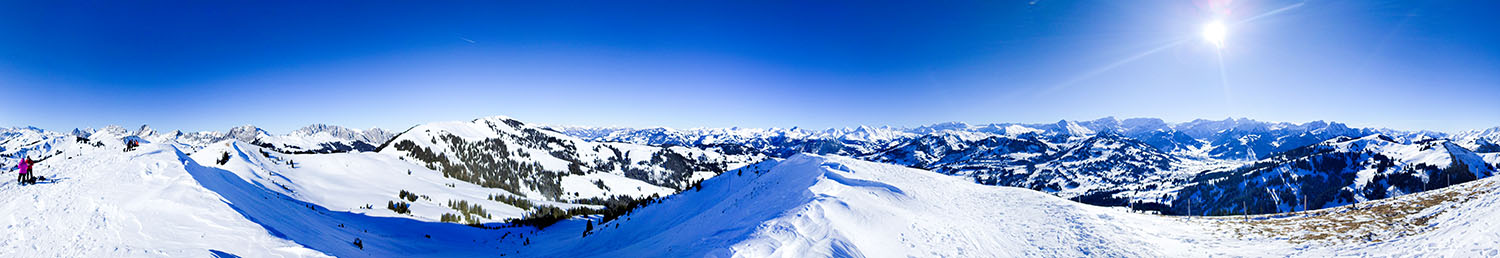
\includegraphics[width=\textwidth]{img/alps/alps_panorama.jpg}
	\caption[Motvation Alpen Panorama]
	{Motivation Alpen Panorama}
\end{figure}
\noindent
Ich bin kein Extrembergsteiger. Ich geniesse die Schweizer Alpen, bin aber nie in hohen(3000m+) und gefährlichen Regionen unterwegs. Die Schneebedingungen während meiner Touren sind meist ideal. Die Gefahr ist minimal. Nur selten werden Themen wie Lawinen und daraus resultierendes Unfallverhalten in der Gruppe diskutiert.\\[0.3cm]
An eben diesem Tag stellten wir uns die Frage: Was wäre wenn? Was wäre passiert, wenn wir von einer Lawine verschüttet worden wären? Wer hätte uns gesucht? Hätte uns überhaupt jemand gesucht? Wie lange würde es dauern bis die Rettungskräfte eintreffen? Wäre das Handynetz verfügbar gewesen? Tausende von Fragen ergaben sich.\\[0.3cm]\
Diese Thematik beschäftigte mich noch lange. Als es darum ging ein Thema für das Bachelor Thesis Vorprojekt (Projekt 2) auszusuchen, wollte ich mich weiter mit diesen Fragen auseinandersetzen. Dank meinem Studium und der gewählten Fachrichtung 'Mobile Computing' hatte ich bereits mehrere Ideen wie man diese Problematik angehen könnte. Das Projekt ATAS war geboren. Meine Vorstellung war es ein System zu erstellen, welches Personen in solchen Situation unterstützen, mehr noch, solche Situationen verhindern sollte.\\[0.3cm]

\chapter{Einleitung}
Ein Gipfel gehört dir erst, wenn du wieder unten bist - denn vorher gehörst du ihm.\\[0.3cm]
\textbf{Hans lander, Italienischer Bergsteiger\cite{kammerlander}} \\[0.5cm]
\noindent
Die Berge sind eine faszinierende Landschaft. Viele Menschen gehen wandern, Ski fahren oder gehen Eisklettern. Die Anzahl der möglichen Aktivitäten ist schier grenzenlos. Immer wieder kommt es in dieser Idylle zu schweren Unfällen, ausgelöst durch Steinschläge, Lawinen oder Abstürze der Bergsteigenden. Der Schweizer Alpen Club (SAC) führt dazu eine jährliche Statistik \cite{sacaccident}. Nachfolgend ein kleiner Auszug aus der Bergunfallstatistik 2016. Die Grafik zeigt eine Übersicht der Anzahl Situationen bei welchen ein Rettungsdienst ausrücken musste. Zu den Rettungsdiensten zählt beispielsweise die REGA.\\
\begin{figure}[H]
	\centering
	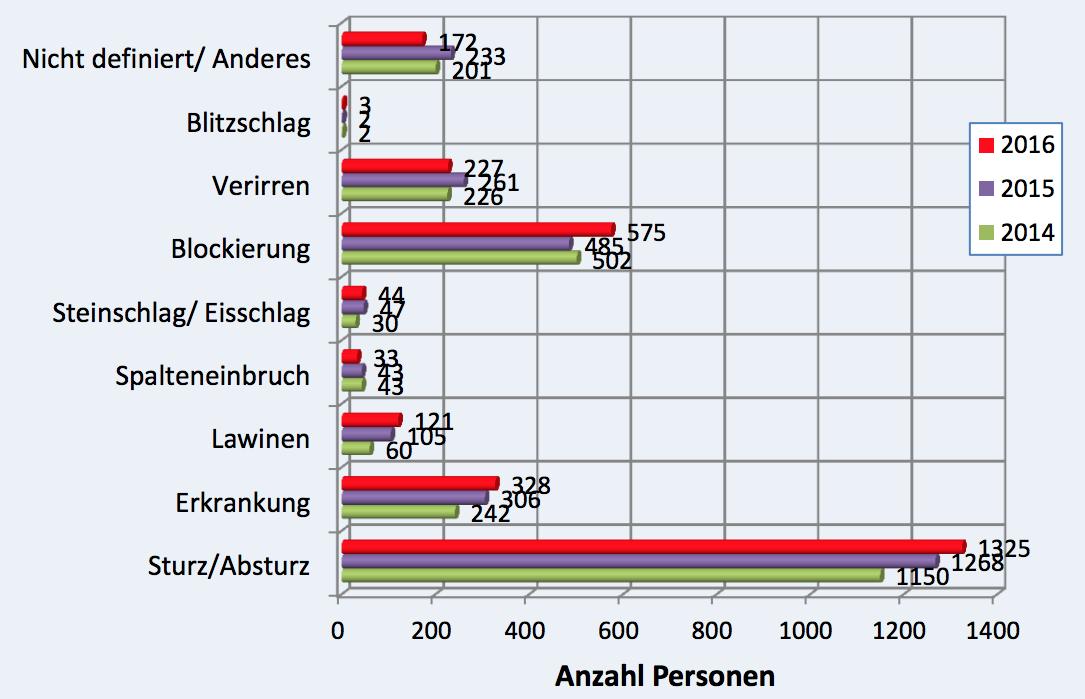
\includegraphics[width=\textwidth]{img/alps/sac_accidentstatistic_2016_reason.png}
	\caption[Bergunfallstatistik 2016 - Notfallsituationen nach Unrsachen]
	{Bergunfallstatistik 2016 - Notfallsituationen nach Ursachen: Quelle: Webseite SAC \cite{sacaccident}}
\end{figure}
\noindent
Die Vorfälle sind nach Ursache gegliedert. Zusammengefasst ergeben sich 2828 Notsituationen. 178 endeten tödlich.
\section{Lawinen}
Ein geringer aber sehr tragischer Anteil davon machen Lawinen aus. Wird eine Person inert 15 Minuten geborgen, Leben noch 90\% der Betroffenen. Man spricht auch von der Überlebensphase. Nach 15 Minuten folgt die Erstickungsphase, die Überlebenschancen schwinden auf geringe 30\%. Je schneller ein Rettungsdienst alarmiert werden kann, desto höher sind die Überlebenschancen \cite{avalancheaccident}. 

\newpage
\section{Projektidee}
Stellen Sie sich ein kleines mobiles Gerät vor, nachfolgend Tracker genannt, welches an Skifahrern, Wanderer usw. abgegeben werden kann. Das Gerät sendet die Position der Person an einen Empfänger. Der Empfänger wird bei der Talstation oder im nächsten Bergdorf montiert. Die Daten werden von einer Software gesammelt und analysiert. Die Administratoren des Systems, beispielsweise die REGA, können in Echtzeit über eine Webseite die aktuelle Position der Personen in den Bergen mitverfolgen und überwachen.

\section{Vorarbeiten}
Das Projekt 2 ist eine Projektarbeit welche im Laufe des Informatikstudiums absolviert wird. Diese Arbeit habe ich im vorhergehenden Semester (Frühlingssemester 2017) durchgeführt. Ziel dieses Projektes, war es das in der Einleitung beschriebene System technisch zu konzeptionieren.\\[0.3cm]
Diese Bachelor Thesis baut auf den Erkenntnissen und Resultaten aus dem Projekt 2 auf.

\section{Aufgabenstellung}
Ziel der Bachelorarbeit soll es sein, dass während dem Projekt2 aufgebaute System intensiv zu testen und zu verbessern. Das Wissen um die verwendeten Technologien soll vertieft werden. Die Arbeit umfasst die folgenden Aufgaben:
\begin{itemize}
\item
Der Tracker soll in realer Umgebung getestet werden bspw. während einer Wanderung. Die Messdaten werden erfasst und analysiert.
\item Der Tracker Prototyp soll verbessert werden. Die dazu erforderlichen Massnahmen werden während der Bachelorarbeit spezifiziert und umgesetzt. Am Ende der Arbeit soll eine klare Aussage gemacht werden können, ob das erdachte System praxistauglich ist.
\end{itemize}

\section{Rahmenbedingungen}
Die Rahmenbedingungen dieses Projektes wurden gemeinsam mit dem Betreuer definiert:
\begin{itemize}
\item Die Bachelorarbeit baut auf der Arbeit des Projekt 2 auf. Die erstellte Hard und Software wird weiterverwendet.
\item Als Programmiersprache soll C/C++ verwendet werden.
\item Auf den Einsatz eines Betriebssystems auf dem Tracker Gerät verzichtet werden.
\end{itemize}

\section{Technologien}
Sie als Leser denken nun vielleicht: "Das ist überflüssig. Ich habe doch mein Handy für so etwas? Schreib doch eine App!". Diese Aussage mag auf die touristischen Wander- und Skigebiete zutreffen. Der Empfang ist meistens wunderbar. Verlassen wir diese 'sicheren' Orte und bewegen uns aber in höheren Lagen, wird der Empfang mit dem Handy immer schlechter oder existiert gar nicht. \bigskip \\
Aus diesem Grund mussten für dieses Projekt andere Technologien gefunden werden. In diesem Projekt werden folgenden Technologien eingesetzt:
\gls{MQTT}, \gls{LoRa}, \gls{LoRaWan}, \gls{TTN} (The Things Network)\bigskip \\
Die verwendeten Technologien und der Grund für deren Einsatz werden im Kapitel 'Technologien' genauer erklärt.

\section{Anwendungsfälle}
Dieser Abschnitt soll Ihnen erläutern, wie das ATAS System genutzt werden kann.
\begin{itemize}
	\item 
	Wenn in den Bergen eine Lawine ausgelöst wird, kann deren Position mit den Positionen der Tracker verglichen werden. Befindet sich ein Tracker in der Gefahrenzone, kann die Rettungsmannschaft sofort reagieren und ausrücken. Dieser Prozess läuft sofort ab und kann dabei die Überlebenschance der Opfer erhöhen. 
	\item 
	Wurden Personen von der Lawine begraben und der Tracker bleibt funktionstüchtig, könnte das Gerät die Position weiterhin senden. Kombiniert mit modernen Lawinensuchgeräten können die Einsatzkräfte gezielter nach Überlebenden suchen. Wenn keine Übertragung mehr möglich ist, wissen die Überwacher zumindest den letzten Aufenthaltsort. Das ATAS System hat nicht das Ziel Lawinensuchgeräte zu ersetzen, es ist eher als Ergänzung zu verstehen. 
	\item 
	Bewegt sich  ein Tracker auf eine Gefahrenzone zu, beispielsweise ein Gebiet mit erhöhter Steinschlaggefahr, könnte die Person frühzeitig davor gewarnt werden. 
	\item 
	Ist es zu einem Unfall gekommen, kann der Alpinist mittels Tracker ein Notsignal absetzen. Dazu muss der Benutzer nur auf den Notfallknopf drücken.
\end{itemize}

\chapter{Systembeschreibung - Grob}
Um die nachfolgenden Kapitel zu verstehen, ist es sehr wichtig, sich mit der im Projekt 2 erstellten Systemarchitektur und die Terminologie vertraut zu machen. Die Architektur wurde im Vergleich zum Projekt 2 um einige Komponenten ergänzt. Der Link zur Projektarbeit kann im Anhang gefunden werden.\\[0.3cm]
Dieser Abschnitt bietet Ihnen einen groben Überblick über die Benutzer, die Komponenten und deren Beziehung innerhalb des ATAS Systems. Alle Einheiten werden auf den nachfolgenden Seiten detailliert beschrieben.

\newpage
\section{Diagram}
Grobes Schema des ATAS Systems. Auf der nachfolgenden Seiten sind die einzelnen Komponenten im Detail beschrieben.\\[0.3cm]
\begin{figure}[H]
	\centering
	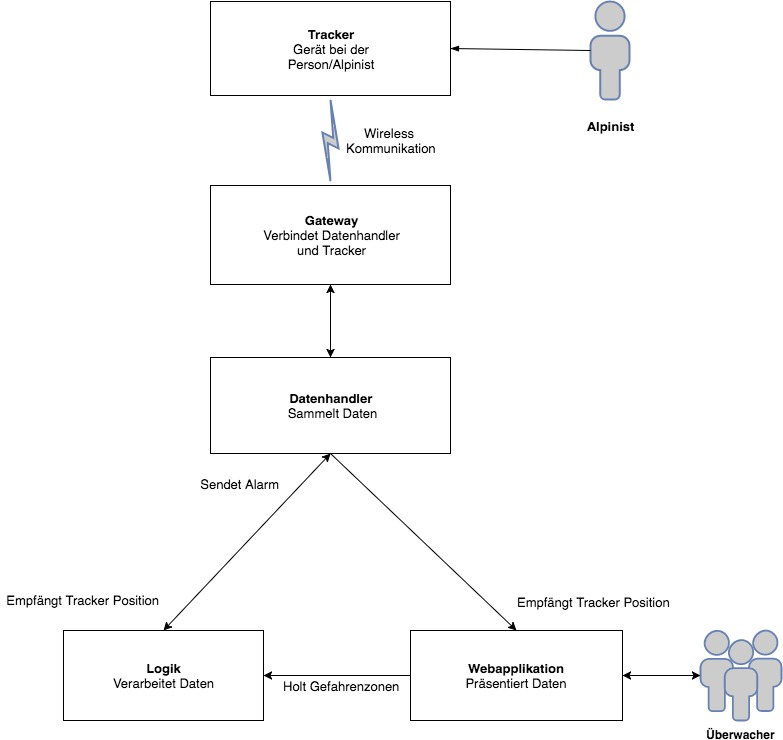
\includegraphics[width=\textwidth]{img/system/ATAS_SystemOverview_Abstract_BA.jpg}
	\caption[ATAS Schema Grob]
	{ATAS Schema Grob}
\end{figure}

\newpage
\section{Benutzer}
Die nachfolgenden Gruppen wurden als Benutzer des Systems identifiziert.

\subsection{Aplinist}
Alpinist wird als Generalisierung für Personen, welche sich in den Bergen aufhalten verwendet. Dazu gehören bspw. Wanderer, Skifahrer, Bergbauern usw.

\subsection{Überwacher}
Rettungsdienste wie bspw. die REGA oder die AirGlacier. Spitäler oder die lokalen Tourismusbehörden.

\section{Komponenten}
Das ATAS System besteht aus den nachfolgenden aufgelisteten Komponenten. Komponenten können Hardware oder Software sein.

\subsection{Tracker}
Stellen Sie sich ein kleines mobiles Gerät vor. Nachfolgend nennen wir dieses Gerät Tracker. Der Alpinist trägt den Tracker bei sich bspw. in einem Rucksack. Der Tracker zeichnet auf wo sich die Person momentan befindet\\ [0.3cm] 
Der Tracker verfügt über ein Display, Schalter, GPS Modul, Kommunikationsmodul und einen Lautsprecher.\\ [0.3cm]
Der Tracker überträgt folgende Daten:
\begin{itemize}
	\item GPS Position des Trackers
	\item Notrufsignale
\end{itemize}
Befindet sich der Tracker in einer Gefahrenzone, wird die Person über den Bildschirm und mit einem Tonsignal alarmiert.
\subsection{Gateway}
Ein Gerät welches mit den Trackern bidirektional kommuniziert. Der Gateway wird an einem Ort nahe den Bergen installiert. Als mögliche Orte kommt ein Dorf im Tal oder eine Talstation in Frage. Der Gateway sendet die empfangenen Daten an einen zentralen Datenmanager, nachfolgend \textbf{Datenhandler} genannt, weiter.

\subsection{Datenhandler}
Sammelt und speichert Daten. Der Datenhandler kommuniziert mit den Gateways. Zusätzlich bietet der Datenhandler ein Interface zum Abfragen und senden von Daten an die Tracker.

\subsection{Webapplikation}
Die Überwacher nutzen eine Webapplikation zum interagieren mit dem ATAS System. Die Webseite bietet folgende Funktionalitäten
\begin{itemize}
	\item
		Zeigt die Position der Tracker auf einer Karte an. 
	\item
		Mittels der Webapp können Gefahrenzonen hinterlegt werden.
	\item 
		Zeigt an, ob sich ein Tracker in einer Gefahrenzone aufhält oder ein Notrufsignal abgesetzt hat.	
\end{itemize}

\subsection{Logik}
Die Logik umfasst Software welche berechnet, ob sich ein Tracker in einer Gefahrenzone aufhält. Wenn sich der Tracker in einer Gefahrenzone aufhält, senden das System einen Alarm an den Tracker. Das Signal gelangt via Datenhandler und Gateway zum Tracker.

\section{Begriffe}
\subsection{Gefahrenzonen}
Wie in der Einleitung beschrieben, stellt der Schweizer Alpen Club Informationen zu Rettungseinsätzen zur Verfügung. Aufgrund der Statistiken wurden die folgenden Gefahren identifiziert vor welchen das ATAS System warnen soll:
\begin{itemize}
	\item Lawinen
	\item Steinschlag
	\item Gletscherspalten
	\item Schneestürme
\end{itemize}

\chapter{Evaluation Technologie}
In diesem Kapitel wird genauer auf die eingesetzten Technologien eingegangen. Es wird beschrieben, wofür und weshalb diese eingesetzt werden. 

\section{Wireless Datenkommunikation}
Zu beginn dieses Projektes musste festgelegt werden, welche Technologie für die Datenübertragung verwendet werden soll. Nachfolgend werden drei mögliche Technologien analysiert. Die Technologien sind für den Einsatz im IoT Bereich optimiert. Die Übertragung benötigt wenig Energie, hat eine hohe Reichweite und meist eine geringe Bandbreite.

\subsection{Sigfox}
Sigfox ist eine \gls{LPWAN} (Low Power Wide Area Network) Lösung welche vom Netzwerk Design eher an ein herkömmliches Mobilfunknetz erinnert. Sigfox ist ein geschlossenes System. Wurde das Gebiet mit Sigfox erschlossen, kann das Netzwerk gegen Bezahlung mitbenutzt werden. Der Aufbau einer eigenen Antenne scheint nicht möglich. 

\subsubsection{Vorteile}
\begin{itemize}
	\item Durch den geringen Energiebedarf halten batteriebetriebene Geräte länger
	\item Grosse Reichweite in nicht bebauten Gebieten, bis zu 40km
	\item Bandbreite, ca. 100b/s
\end{itemize}
\subsubsection{Nachteile}
\begin{itemize}
	\item Bis heute (15.1.2018) wurde die Schweiz von Sigfox noch nicht erschlossen.
	\item Limitierung in der Zahl der Nachrichten die gesendet werden können. Zum Endgerät (Downlink) 140x 12 Byte. Vom Endgerät an das Netzwerk (Uplink) 4x 8 Byte
	\item Sigfox wird als Service Angeboten. Für den Dienst muss bezahlt werden.
\end{itemize}

\subsection{LoRa}
LoRa steht für Long Range und ist eine Wide-Area Netzwerk Lösung. Die Lösung besteht meist aus zwei Schichten
\begin{itemize}
	\item LoRa. Link Layer, Physikalische Schicht. LoRa definiert, wie die Daten im Medium (Luft) übertragen werden.
	\item LoRaWan. Media Access Control (MAC) Protokoll. Definiert das Format der Daten.
\end{itemize}
LoRa hat drei Hauptmerkmale. Der Energieverbrauch ist gering (low-power), die Reichweite ist hoch (long-range) und die maximale Übertragungsrate ist gering (low-throughput).
\subsubsection{Vorteile}
\begin{itemize}
	\item Durch den geringen Energiebedarf halten batteriebetriebene Geräte länger
	\item Die Kosten für die Installation eines Lora resp. LoRaWan Gateways sind gering +- 300.-
	\item Grosse Reichweite in nicht bebauten Gebieten, bis zu 15km
	\item Geringe Störanfälligkeit durch den Einsatz von Spreading Factors resp. Chirp Spread Spectrum (CSS)
	\item Frequenzbereich im ISM Band. Lizenzfreie Frequenzbereiche. Es müssen keine Gebühren bezahlt werden.
	\item Grosses Link Budget, +14dB Sender und -137db Empfänger Sensitivität $\rightarrow$ 151dB
	\item Erfreut sich grosser Beliebtheit. Immer mehr Informationen und hilfreiche Ressourcen sind im Internet zu finden.
\end{itemize}
\subsubsection{Nachteile}
\begin{itemize}
	\item Geringe Verbreitung, je nach Region
	\item Geringe Bandbreite, von 0.3Kb/s zu 27Kb/s mit CSS, 50Kb/s mit FSK Modulation \cite{loradatarate}
\end{itemize}

\newpage
\subsection{NB-IOT, LTE Cat M1}
NB-IOT (Narrowband - Internet of Things) und LTE Cat M1 wurden als Konkurrenz zu den populären Lösungen LoRa und Sigfox entwickelt. Auf diese Netzwerke wird hier vorerst nicht eingegangen. Die Standards wurden erst kürzlich von der Industrie aufgegriffen und werden langsam eingeführt. Die Swisscom plant erste Tests gegen Ende 2017. Der Rollout für die Nutzer soll im Frühjahr 2018 beginnen \cite{swisscomnbiot}.

\subsection{Entscheid}
Sigfox scheidet als mögliche Technolgie aus. Die Angaben zur Reichweite sind zwar sehr beeindruckend, die Beschränkung in der Anzahl der Down- und Uplinks macht es leider für das ATAS System unbrauchbar. Mit nur 140 Nachrichten pro Tag, kann die Position des Trackers nicht häufig genug ermittelt werden.\\[0.3cm]
NB-IOT \& LTE Cat M1 scheinen eine potente Mobilfunklösung für den IoT Bereich zu sein. Die Zukunft wird zeigen, ob sich die Technologie gegen die bestehende Konkurrenz behaupten kann.\\[0.3cm]
Bleibt noch LoRa. LoRa überzeugt mit der guten Reichweite und der kleinen Belastung der Batterie. Für das System ATAS wir LoRa als Datenkommunikationslösung eingesetzt.

\newpage
\section{LoRa}
Um das Projekt durchzuführen, musste das Wissen zum Thema LoRa vertieft werden.

\subsection{LoRa Modulation}
LoRa unterstützt zwei Modulationsarten, das simple Frequency Shift Key (FSK) und das Chirp Spread Spectrum (CSS) Verfahren. In dieser Arbeit setzen wir den Fokus auf CSS.\\[0.3cm]
Ein Chirp ist ein Sinussignal, bei welchem über die Zeit die Frequenz erhöht oder reduziert wird.
\begin{figure}[H]
	\centering
	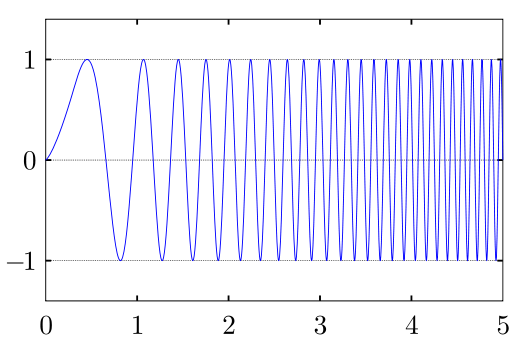
\includegraphics[width=0.6\textwidth]{img/lora/upchirp.png}
	\caption[Beispiel Upchirp]
	{Beispiel Upchirp, Quelle: Wikipedia CSS \cite{CSS}}
\end{figure}
\noindent
Wie im Bild ersichtlich erhöht sich die Frequenz des Signals. Bei einer Erhöhung der Frequenz reden wir von einem Upchirp, bei einer Reduktion von einem Downchirp. Das Chirp Signal ist das Trägersignal und wird anschließend verwendet um die Daten zu kodieren.

\subsubsection{Bandbreite}
Bei LoRa haben wir die Möglichkeit zwischen drei Bandbreiten zu wählen. Die Bandbreite definiert die Grösse des Bereiches der zwischen der kleinsten und der grössten möglichen Frequenz liegt. Die Bandbreiten sind 125kHz, 250kHz und 500kHz. In Europa sind nur die Bandbreiten 125KHz und 250KHz zulässig \cite{lorabandwitdh}. 

\newpage
\subsubsection{Spreading Factor}
Zwei Parameter beeinflussen das Chirp modulierte Signal. Erstens die Bandbreite und zweitens die sog. Sweep Rate.

\begin{figure}[H]
	\centering
	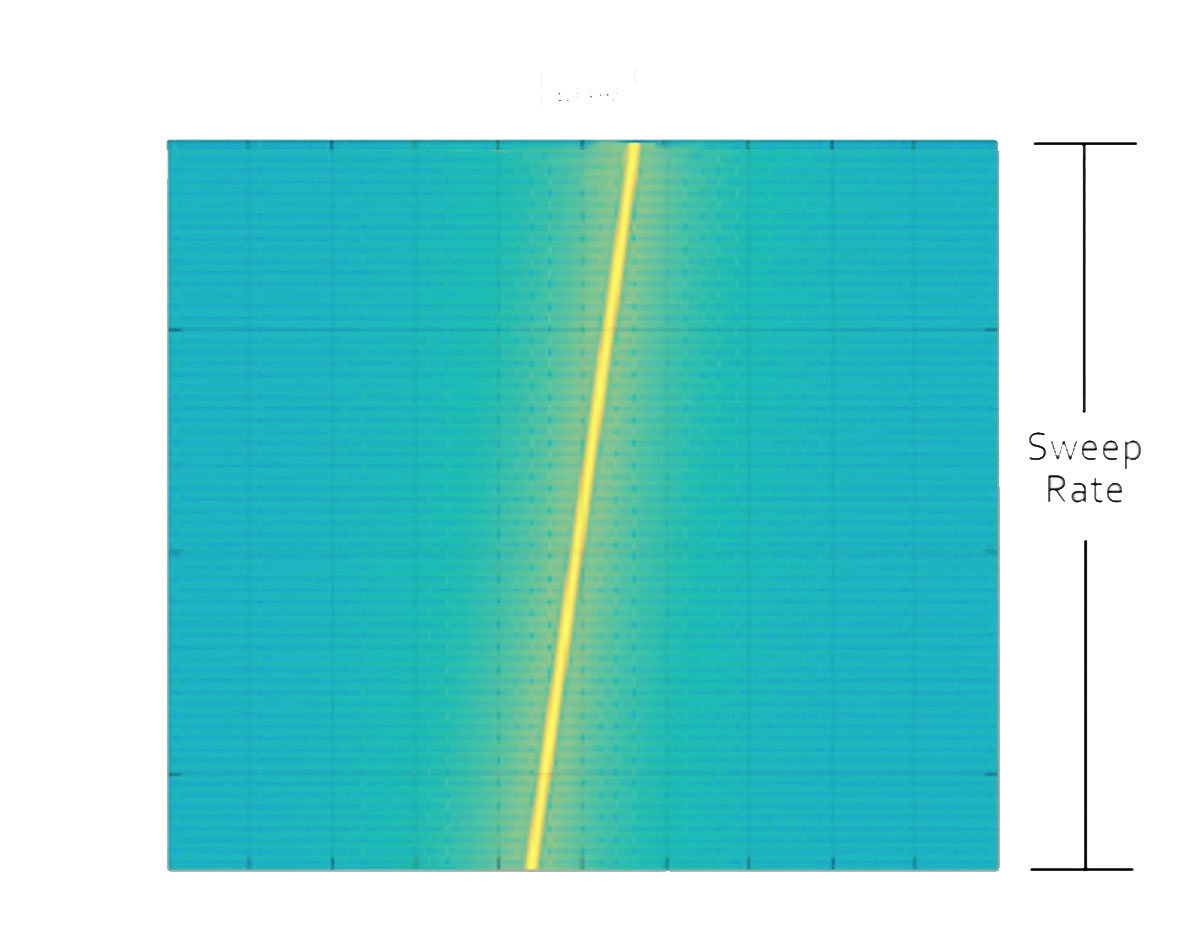
\includegraphics[width=0.6\textwidth]{img/lora/chirp.jpg}
	\caption[Wasserfall Darstellung: Chirp Parameter]
	{Wasserfall Darstellung: Chirp Parameter, Quelle: Youtube Video LoRa \cite{lorabandwidth}}
\end{figure}

\noindent
Ein weiteres Beispiel eines Upchirps. Bei diesem Signal wird 125kHz verwendet. Die Frequenz nimmt gegen Links zu. Der gelbe Strich zeigt uns die momentane Frequenz zum Zeitpunk x. Nach erreichen der maximalen Frequenz folgt der nächste Chirp. Dieses Intervall wird auch Sweep Rate genannt.

\newpage
\noindent
Die Einstellungsmöglichkeiten der Parameter wurden in Europa zu Gruppen, sogenannten Spreading Factors zusammengefasst. Es gibt die Faktoren SF7-SF12.

\begin{figure}[H]
	\centering
	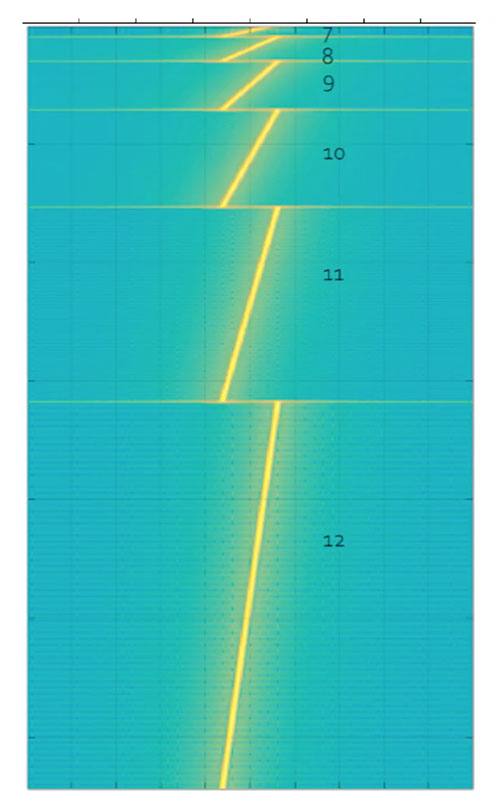
\includegraphics[width=0.48\textwidth]{img/lora/spreadingfactors.jpg}
	\caption[Wasserfall Darstellung: Spreadingfactors 7-12]
	{Wasserfall Darstellung: Spreadingfactors 7-12, Quelle: Youtube Video LoRa \cite{lorabandwidth}}
\end{figure}

\noindent
Wie in der Grafik ersichtlich, ist die Sweep Rate bei SF12 viel langsamer als bei SF7. Pro Schritt zwischen den SF (SF7 zu SF8) halbiert sich der Datendurchsatz. Das Senden einer Nachricht dauert länger, ist aber einfacher zu dekodieren. Das Signal wird weniger anfällig gegenüber Störungen und kann damit über eine grössere Distanz übertragen werden. Müssen 'grössere' Datenmengen oder in einem kleineren Zeitintervall versendet werden, bietet es sich an einen kleineren Spreadingfactor zu wählen (7-9). Sollen grosse Distanzen überwunden werden oder gibt es in der Region viele Störsignale, sollte ein hoher Spreadingfactor (10-12) verwendet werden.

\newpage
\subsection{Regulierungen}
Für die Schweiz und in vielen Teilen Europas gilt für die Nutzung von LoRa die Regelung ERC/REC 70-03 \cite{regulations}. Zusammengestellt wurden die Regulationen von der CEPT (European Conference of Postal and Telecommunications). Die Schweiz ist Mitglied dieser Organisation. Die Standardisierung selbst hat die Organisation ETSI (EN300.220) übernommen. Das Dokument beschreibt die verwendbaren Frequenzen, die maximale Übertragungsleistung (dbm) sowie den Duty Cycle.\\[0.3cm]
Die Regulationen wurden in dieser Projektarbeit eingehalten. Die maximale Sendeleistung von 25mW resp. 14dbm wurde während den Tests nicht überschritten.

\subsection{Datenübertragungsrate}
Der Duty Cycle und die damit verbundene Airtime haben einen grossen Einfluss auf die Datenübertragungsrate. 
\subsubsection{Duty Cycle}
Der Duty Cycle oder zu Deutsch 'Auslastungsgrad' beschreibt, wie lange ein Signal oder ein System aktiv ist \cite{wikiduty}. In unserem System beispielsweise wie lange der Tracker sendet. Dieser Prozentsatz wird meist vom Gesetzgeber festgelegt. Wir müssen uns an die Einschränkungen halten, was wiederum bedeutet, dass wir nicht konstant Daten senden dürfen. Die nachfolgenden Frequenz und Sub-Bänder wurden durch die ETSI definiert und können in Europa verwendet werden\cite{lorawanfreq}.

\begin{tabularx}{\linewidth}{XXXX}
	\textbf{Band} & \textbf{Frequenz} & \textbf{Energieverbrauch} & \textbf{Duty Cycle} \\ \hline
	g &863.0 - 868.0 MHz & 25mW&1\%\\ \hline
	g1 &868.0 - 868.6 MHz & 25mW& 1\%\\ \hline
	g2 &868.7 -869.2 MHz & 25 mW& 0.1\%\\ \hline
	g3 &869.4 - 869.65 MHz & 500mW& 10\%\\ \hline
	g4 &869.7 - 870.0 MHz & 5mW/25mW& 1\%\\ \hline
\end{tabularx} 
\noindent
Diese Frequenzbänder gelten für den Einsatz in Kombination mit LoRaWan in Europa. In anderen Regionen der Welt gelten andere Frequenzen. Für das ATAS Projekt wird der Duty Cycle auf 1\% festgelegt. Dies erlaubt uns die nötigen Daten in entsprechender kurzen Zeit zu übermitteln.

\newpage
\subsubsection{Airtime}
Die Airtime definiert, wie lange es dauert ein Signal vom LoRa Endgerät zum Gateway zu übertragen. Die Airtime ist abhängig von der Menge der zu übertragenden Daten und dem verwendeten Spreading Factor.\\[0.3cm]
Die untenstehende Grafik verbildlicht diesen Zusammenhang.
\begin{figure}[H]
	\centering
	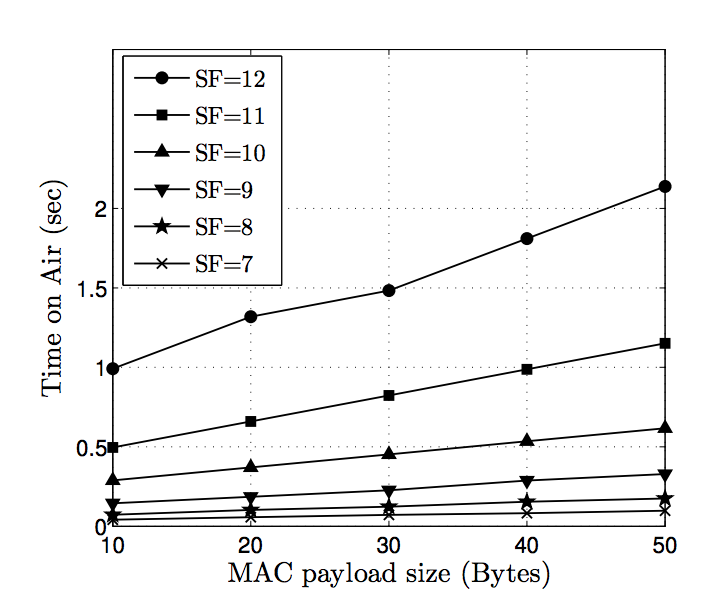
\includegraphics[width=0.6\textwidth]{img/lora/timeonair.png}
	\caption[Time on Air]
	{Time on Air, Quelle: Understanding the Limits of LoRaWAN \cite{loradatarate}}
\end{figure}
\noindent
Je höher der Spreadingfactor, desto länger dauert die Übertragung. Auf die genaue Berechnung der Airtime und der gesamten Payload wird hier nicht weiter eingegangen.

\subsubsection{Berechnung}
Wir wissen nun also, dass wir nicht beliebig oft senden dürfen. Weiter wissen wir, dass die Airtime im Endeffekt bestimmt wie lange die Übertragung dauert. Die Formel lautet nun wie folgt.
\begin{equation*}time = \frac{airtime}{dutycylce * 1000}\end{equation*}
Im Abschnitt 'Testing' werden wir später genau ermitteln wie häufig wir mit dem ATAS System senden können.

\newpage
\subsection{Coding Rate}
Die Coding Rate definiert die Error Kodierungsrate. Eine höhere Kodierungsrate ermöglicht es das Signal auch bei Störungen (Noise) zu rekonstruieren. Ein erhöhen der Coding Rate verursacht eine grössere Menge an Daten die gesendet werden $\rightarrow$ Overhead. Nutzdaten (bit) werden mehrmals übertragen. Ein Signal beinhaltet also redundante Informationen. Mögliche Coding Rate Werte im LoRa Umfeld sind 4/5 und 4/8.
\begin{exmp}
	Annahme: Wir setzen die Coding Rate auf 4/8\\
	8 - 4 = 4, d.H bei 4 Bit Nützlichen Informationen fügen wir nochmals 4 Bit redundante Informationen hinzu.
\end{exmp}
\noindent
Um ein möglichst gutes Signal zu erhalten, soll im ATAS System die Kodierungsrate auf 4/8 festgelegt werden.

\newpage
\section{LoRaWan}
LoRaWan ist ein Protokoll welches auf LoRa aufbaut. Das Protokoll definiert die Struktur der Daten die gesendet werden.
\subsection{Netzwerk Architektur}
\begin{figure}[H]
	\centering
	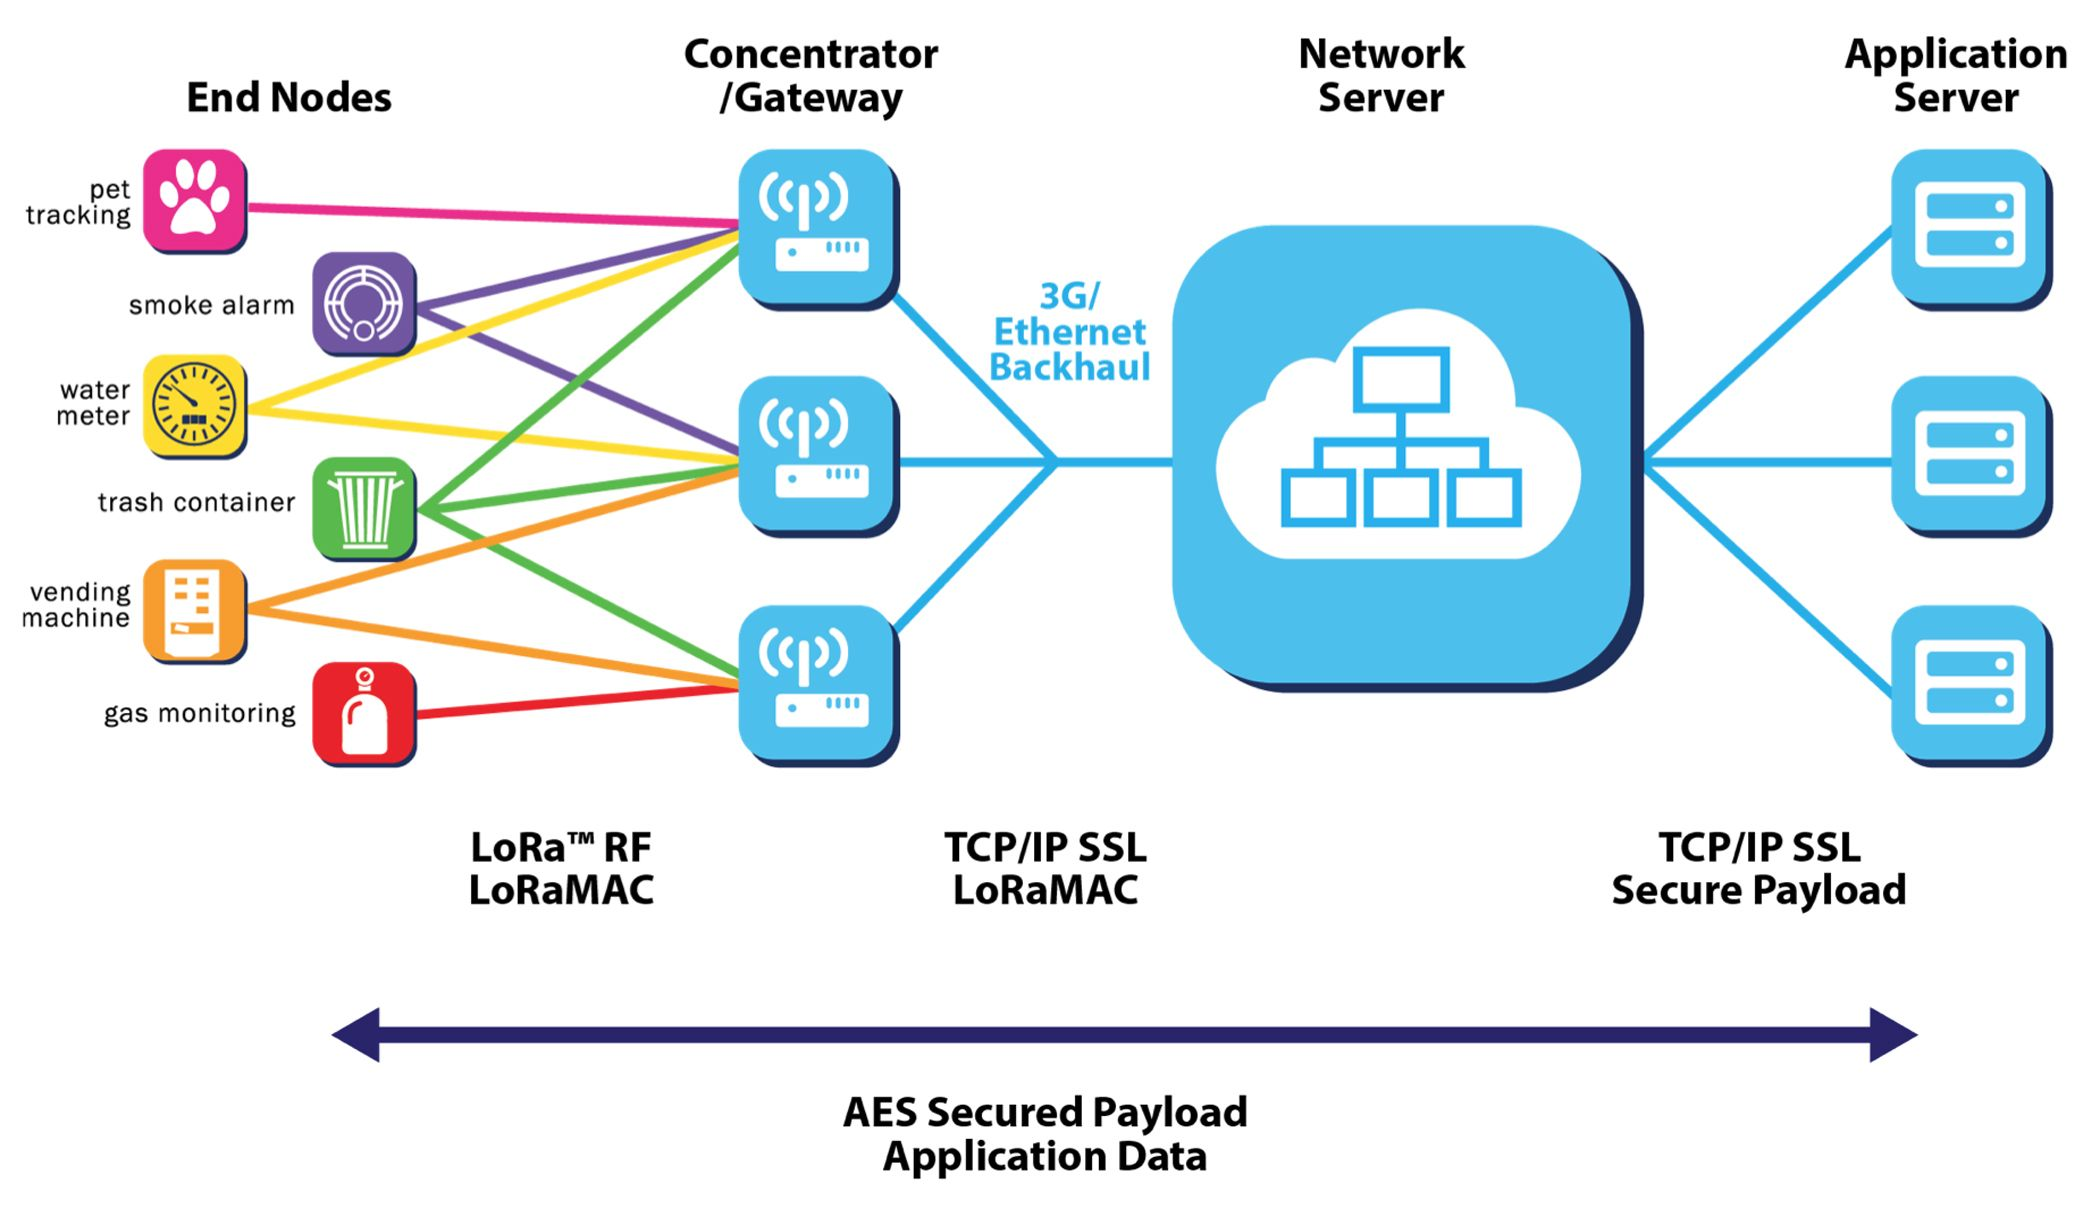
\includegraphics[width=\textwidth]{img/lora/lorawantopology.jpg}
	\caption[LoRaWan Architektur]
	{LoRaWan Architektur, Quelle: Blog \cite{lorawanarchitecture}}
\end{figure} 
Ein LoRaWan Netzwerk besteht aus mehreren Komponenten\\[0.3cm]
\textbf{Die End Nodes} sammeln Daten über Sensoren. Das können ganz unterschiedliche Sachen sein, wie zum Beispiel Feuchtigkeit in einem Raum. Die End Nodes senden Daten an die Empfänger (Gateways, Concentrator) via LoRa. Die Daten werden hier, nicht wie in einem Mobilfunknetz an nur eine Antenne, sonder an alle Empfänger gesendet.\\[0.3cm]
\textbf{Die Gateways} leiten die erhaltenen Informationen weiter an den Netzwerk Server. Die Gateway sind meist mit dem Internet über Kabel oder Wireless verbunden.\\[0.3cm]
\textbf{Der Netzwerk Server} verwaltet die ein-kommenden Datenströme. Doppelte Pakete werden gefiltert und Sicherheitsregeln werden angewandt. Abschliessend sendet der Gateway eine Empfangsbestätigung (Acknowledgement) an den Gateway, dass er die Pakete sauber erhalten hat.\\[0.3cm]
Zum Schluss werden die Daten an die zuständigen \textbf{Applikations Server} weitergeleitet.

\newpage
\subsection{Sicherheit}
Durch bereits eingebaute Sicherheitsmechanismen in LoRaWan sind die übertragenen Daten geschützt. Die Daten werden End zu End mit AES-128Bit verschlüsselt \cite{ttnsecuirty}.

\subsection{Endgerät Verbindungsmethoden}
ABP (Activation By Personalization) und OTAA (Over-The-Air-Activation) sind Verbindungsmethoden für \gls{LoRaWanEndDevice} in einem LoraWan Netzwerk.\cite{jaguar}. Die verwendete Methode definiert also wie sich ein Endgerät mit dem LoRaWan Netzwerk verbindet. \\[0.3cm]
Die beiden Methoden bieten verschiedene Vor und Nachteile.

\subsubsection{ABP}
ABP ist das simplere aber \textbf{weniger sichere} Verfahren. Die Adresse DevAdr sowie die Schlüssel \gls{NetSKey} und des \gls{AppSKey} werden für jedes Endgerät \textbf{einmalig} generiert und fix auf dem Endgerät hinterlegt. Gelingt es einem Angreifer sich Zugang zum Endgerät zu verschaffen, kann er die Schlüssel stehlen, ein zweites Gerät am Netzwerk registrieren, die Identität des Originals annehmen und damit die Daten verfälschen.\\[0.3cm]
Das Gerät muss sich nicht am Netzwerk anmelden. Das Endgerät kann direkt Daten senden. Empfängt ein Gateway die Daten, werden die Keys geprüft und die Kommunikation entsprechend angenommen oder abgelehnt.

\subsubsection{OTAA}
Das Gerät muss sich am Netzwerk anmelden. Dieser Vorgang wird auch Join Prozedur genannt. Die \gls{DevAddr} sowie die Keys NetSKey und AppSKey werden bei jeder Aktivierung des Gerätes \textbf{neu generiert} und an das Endgerät übertragen. Dieses Verfahren ist sicherer. Da es sich hier um eine bidirektionale Kommunikation handelt, müssen die Komponenten (Gateway \& Endgerät) Downlinks unterstützen.\\[0.3cm]
Das Installieren (Deployment) von Endgeräten wird vereinfacht. Das generieren vom AppSKey und NetSKey pro Endgerät entfällt. 

\newpage
\noindent
Die nachfolgende Grafik zeigt auf, wie der Kommunikationsaufbau via OTAA abläuft \cite{jaguar}.
\begin{figure}[H]
	\centering
	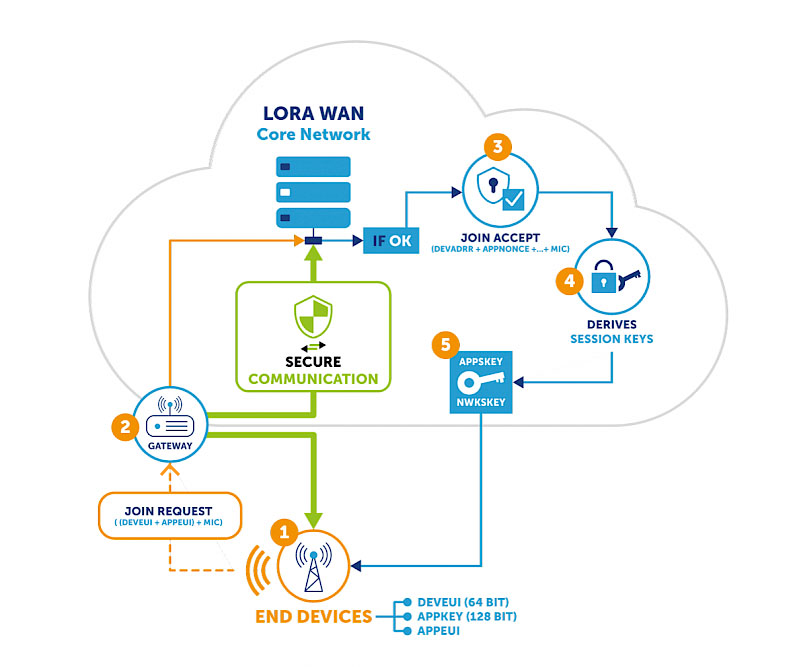
\includegraphics[width=0.9\textwidth]{img/lora/otaa_schema.png}
	\caption[OTAA Ablauf]
	{OTAA Ablauf, Quelle: Webseite Jaguar-Network \protect\cite{jaguar}}
\end{figure}

\begin{enumerate}
	\item Gerät sendet einen Join Request.
	\item Die Gateways empfangen die Anfrage
	\item Das LoRaWan Netzwerk  bspw. TTN prüft die Angaben
	\item Session Keys werden generiert
	\item Keys werden an das Endgerät gesendet und für die zukünftige Kommunikation verwendet
\end{enumerate}

\newpage
\subsubsection{Schlussfolgerung}
Obschon die Sicherheit während diesem Projekt nicht im Vordergrund steht, ist es sicher zukunftsorientierter direkt OTAA einzusetzen. Systeme welche zum Schutz von Personen eingesetzt werden, müssen so sicher wie nur möglich konzeptioniert sein.\\[0.3cm]
Sowohl Endgerät als auch Gateway unterstützen Downlinks, damit gibt es keine technische Hürde der den Einsatz von OTAA verhindern würde. Aus diesem Grund wurde während dem Projekt die Verbindungsmethodik von ABP auf OTAA umgestellt. Damit konnte die Sicherheit des Systems verbessert werden.

\subsection{Frame Counters}
Ein Endgerät besitzt zwei Zähler (FCntUp, FCntDown). Die Zähler werden bei einer Downlinkmessage (FCntDown) resp. Uplinkmessage (FCntUp) erhöht (+1).\\[0.3cm]
Wird eine Reply Attacke durchgeführt d.H. ein Paket nochmals gesendet, wird dieses Paket vom System verworfen. Dies geschieht deshalb, weil das System bereits eine Nachricht mit dem gleichen Framecounter erhalten hat.\\[0.3cm]
Diese zusätzliche Information wird mir beim Testen der Übertragung überaus nützlich sein. Anhand der Nummerierung, kann sehr schnell erkannt werden, ob ein Paket nicht sauber empfangen werden konnte. Bspw. Erhalten wir die Pakete 4,5,7 $\rightarrow$ Paket 6 wurde nicht korrekt übertragen.

\newpage
\subsection{Geräteklassen}
LoRaWan Endgeräte werden in drei Geräteklassen unterteilt \cite{lorawan_classes}. Alle Geräte unterstützen eine bidirektionale Kommunikation. Es können also Daten zum Gateway gesendet wie auch empfangen werden.
\subsubsection{Klasse A}
Alle Geräte der Klasse B und C haben die Funktionalität von Klasse A implementiert. Das Endgerät kann immer Senden. Für den Empfang der Daten gibt es bestimmte Regeln. Nach einem Senden öffnet das Endgerät zwei sogenannte Download Receive Fenster. Während dieser Zeit können Daten Empfangen werden. 

\begin{figure}[H]
	\centering
	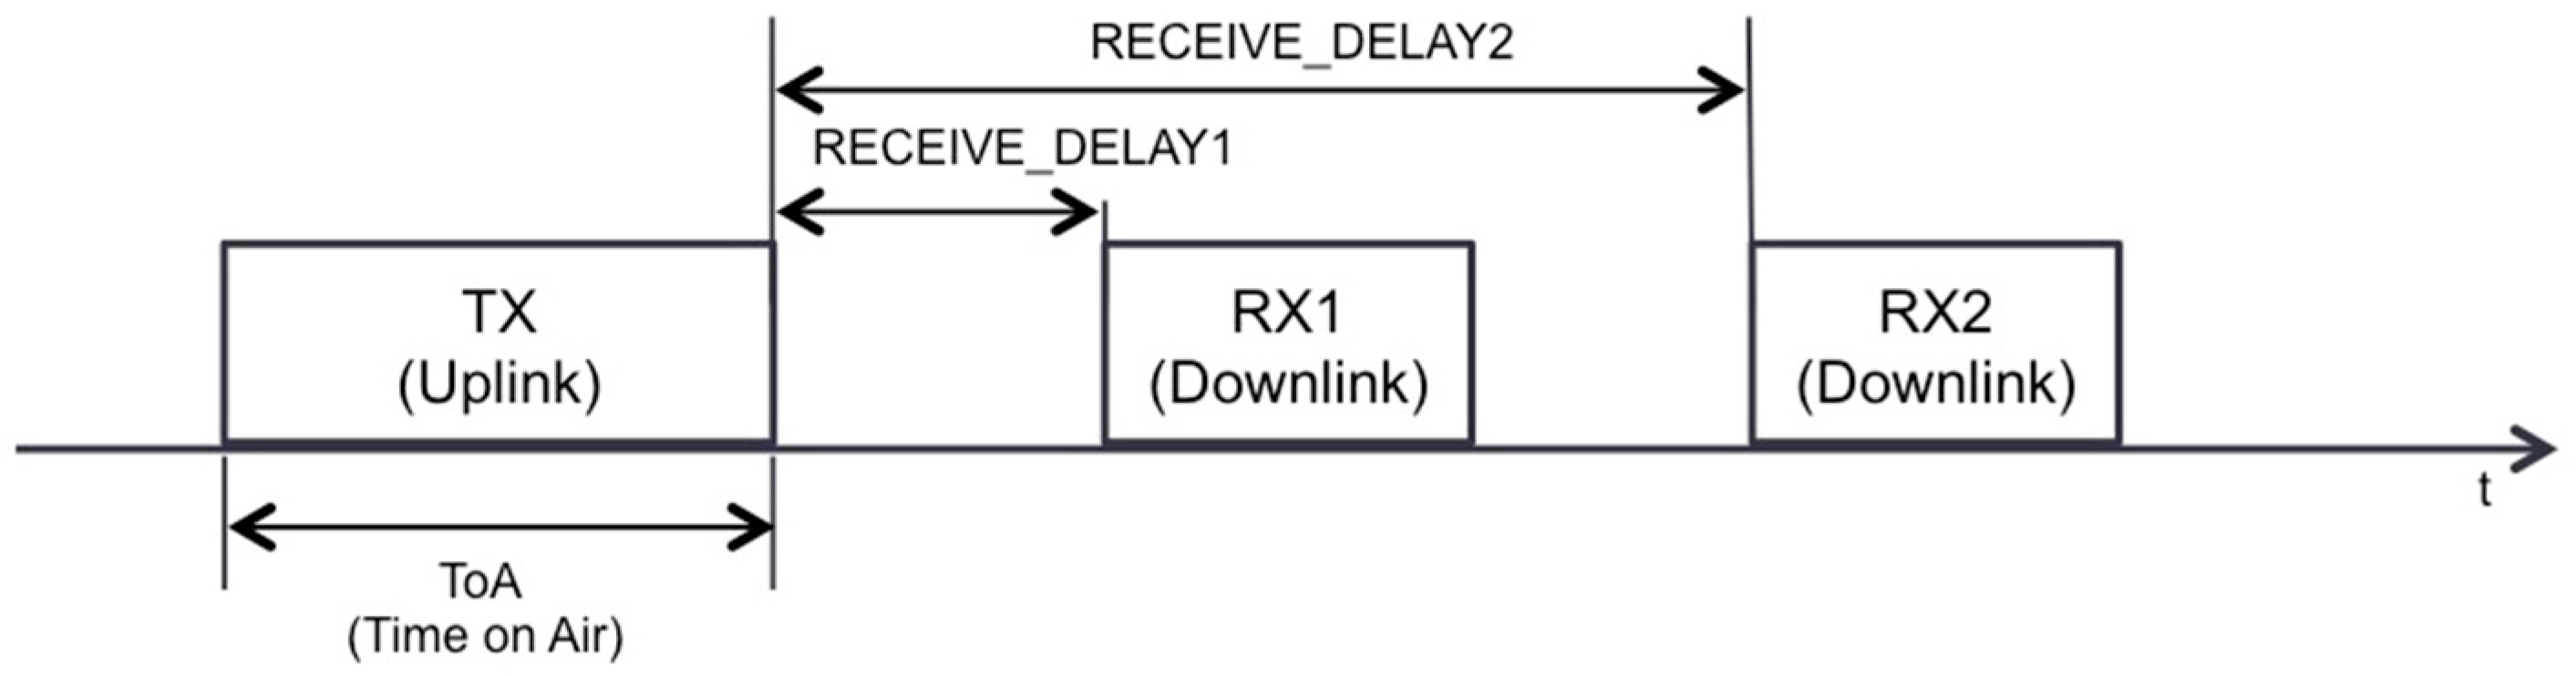
\includegraphics[width=0.9\textwidth]{img/lora/lorawan_class_a.png}
	\caption[LoRaWan Klasse A]
	{LoRaWan Klasse A, Quelle: Webseite \cite{loraclass}}
\end{figure}
\noindent
Werden Daten ausserhalb dieses Zeitfensters geschickt, werden diese nie vom Endgerät empfangen.

\subsubsection{Klasse B}
Ein Klasse B Gerät kann zusätzliche Download Receive Fenster zu definierten Zeiten öffnen. Der Gateway sendet ein Datenpaket (Beacon) an die Endgeräte um die Zeiten zu synchronisieren. Sind die Zeiten synchronisiert, weiss das LoRaWan Netzwerk ganz genau wann ein Endgerät bereit ist Daten zu empfangen. 

\newpage
\subsubsection{Klasse C}
Klasse C Geräte haben ein nahezu permanent geöffnetes Receive Zeitfenster. Nur während einem Sendevorgang wird dieses kurzzeitig geschlossen. Durch diese Eigenschaften ist der Energievierbauch von Klasse C Geräten im Vergleich zu A \& B sehr viel grösser.

\begin{figure}[H]
	\centering
	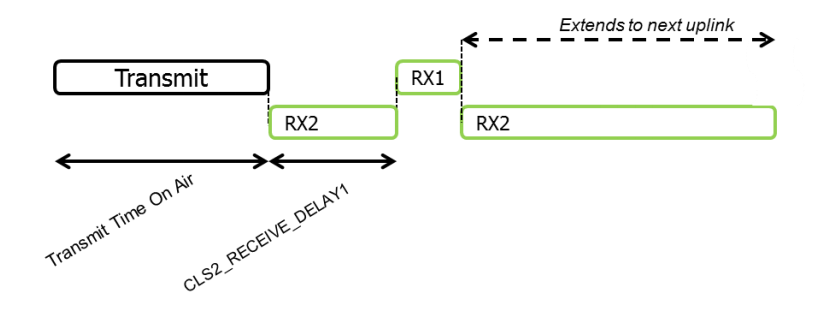
\includegraphics[width=0.9\textwidth]{img/lora/lorawan_class_c.png}
	\caption[LoRaWan Klasse C]
	{LoRaWan Klasse C, Quelle: Webseite \cite{loraclass}}
\end{figure}

\subsubsection{Entscheid}
Der Energieverbrauch von Klasse A Geräten ist im Vergleich von B \& C geringer. Der Tracker muss nicht in der Lage sein, einen Alarm zu jeder Zeit zu empfangen. Klasse A ist genügend. Diese Tatsachen machen den Entscheid sehr einfach. Für die ATAS Tracker werden wir also die Klasse A verwenden. 

\newpage
\subsection{Adaptive Data Rate (ADR)}
Ist Adaptive Data Rate aktiv (ADR), entscheidet das LoraWan Endgerät selbständig ob und wie die Kommunikation optimiert werden soll. Gemäss TTN \cite{ADRTTN} sollte ADR nur für statische Nodes oder für mobile Nodes zur Erkennung von Stops (keine Bewegung) verwendet werden. Gemäss TTN ist ADR also nicht unbedingt für die ATAS-Tracker geeignet. Die Tracker sind ja meistens in Bewegung bspw. durch Laufen, Ski fahren usw. Dennoch wurde mein Interesse geweckt und ich wollte genauer wissen warum dieses Feature nicht empfohlen wird.\\[0.3cm]
Sobald ein LoraWan Endgerät dem Netzwerk mitteilt, dass es ADR verwenden möchte, beginnt das TTN Daten aufzuzeichnen. Die letzten 20 Messdaten die der Node gesendet hat werden analysiert. Ist der Node nahe dem Gateway wird der Spreadingfactor (SF) heruntergeschraubt bspw. von SF10 auf SF7. Damit wird Airtime und Energie gespart. Entfernt sich der Node vom Gateway wird SNR und damit RSSI schlechter. Das System erhöht nun automatisch  den SF um eine bessere Übertragung sicherzustellen.\\[0.3cm]
Der Einsatz von ADR macht im ATAS System meiner Meinung nach wenig Sinn. Dafür gibt es zwei Gründe:
\begin{itemize}
	\item Die ADR Kommunikation generiert einen Overhead \cite{adroverhead}. Die ADR Kommunikation benötigt jeweils zwei Uplink und eine Downlink Message. 
	\item In der Zeit welche zwischen zwei Uplinks vergeht, kann sich die Umgebung drastisch verändern. Bspw. Der Wanderer hat direkten Sichtkontakt mit dem Gateway. Das System reduziert den Spreadingfactor. 2 Minuten später befindet er sich in einem Waldstück mit einer hohen Signaldämpfung. Die nun gesendeten Uplinks erreichen möglicherweise das Ziel nicht.
\end{itemize}Diee Entwicklung eines eigenen ADR Systems wäre hier die Lösung. Der SF ist grundsätzlich hoch (SF11-SF12) zu halten um eine Übertragung der Daten zu garantieren. Mittels Auswertung der letzten GPS Punkte könnte das System die Geschwindigkeit der Person erkennen. Bewegt er sich langsam (laufen), könnte die Zeit zwischen den einzelnen Uplinks erhöht werden. Damit sparen wir Energie. Bewegt er sich schneller (Ski Fahren) kann die Zeit reduziert werden. 

\newpage
\section{LoRaWan Netzwerk}
\subsection{Evaluation}
Ein eigenes LoRaWan Netzwerk aufzubauen ist möglich, würde aber den Umfang dieser Arbeit sprengen. Aus diesem Grund wurde entschieden auf bereits bestehende Netzwerke zurückzugreifen.\\[0.3cm]
Die Verbreitung von LoRaWan in der Schweiz ist mittlerweile sehr hoch. Unternehmen wie die Swisscom und die Schweizer Post haben begonnen grosse LoRaWan Netzwerke aufzubauen \cite{swisscompost}.\\[0.3cm]
Eine Übersicht über die aktuelle Abdeckung des Swisscom und der Post, Stand (2.11.2017)  \cite{swisscomcoverage}.
\begin{figure}[H]
	\centering
	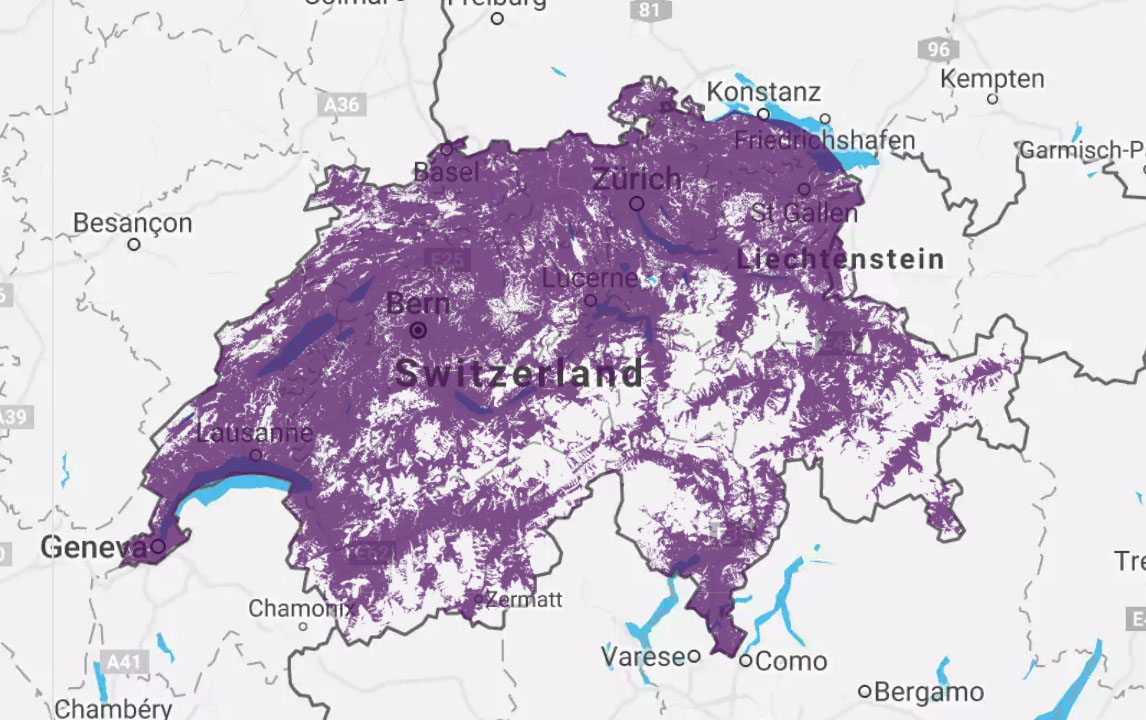
\includegraphics[width=\textwidth]{img/lora/swisscomlorawan.jpg}
	\caption[Swisscom LoRaWan Abdeckung]
	{Swisscom LoRaWan Abdeckung, Quelle: Swisscom LPWAN Webseite \cite{swisscomcoverage}}
\end{figure}
\noindent
Violett steht für Abeckung. Weisse Stellen bedeutet es existiert keine LoRaWan Abdeckung. Wie in der Grafik ersichtlich, sind die Städtischen Gebiete bereits erschlossen. Anders sieht es in den Bergregionen aus. Das Netzwerk der Swisscom und der Post kann somit für das ATAS System nicht verwendet werden.\

\newpage
\subsection{The Things Network, TTN}
Auf anraten von Personen aus dem nahem Umfeld welche sich bereits intensiv mit LoRaWan auseinander gesetzt haben, wird beim ATAS System das Netzwerk 'The Things Network' eingesetzt. The Things Network kurz TTN ist eine LoRaWan Plattform, welche LoRaWan Endgeräte mit Applikationen verbindet. Der Beitritt ist kostenlos. Das Projekt wird von einer grossen Community betrieben. Ein eigener Gateway kann unkompliziert aufgeschaltet und in das Netzwerk integriert werden. 

\subsubsection{Architektur}
Das TTN Netzwerk in sich besteht aus vielen einzelnen Komponenten.
\begin{figure}[H]
	\centering
	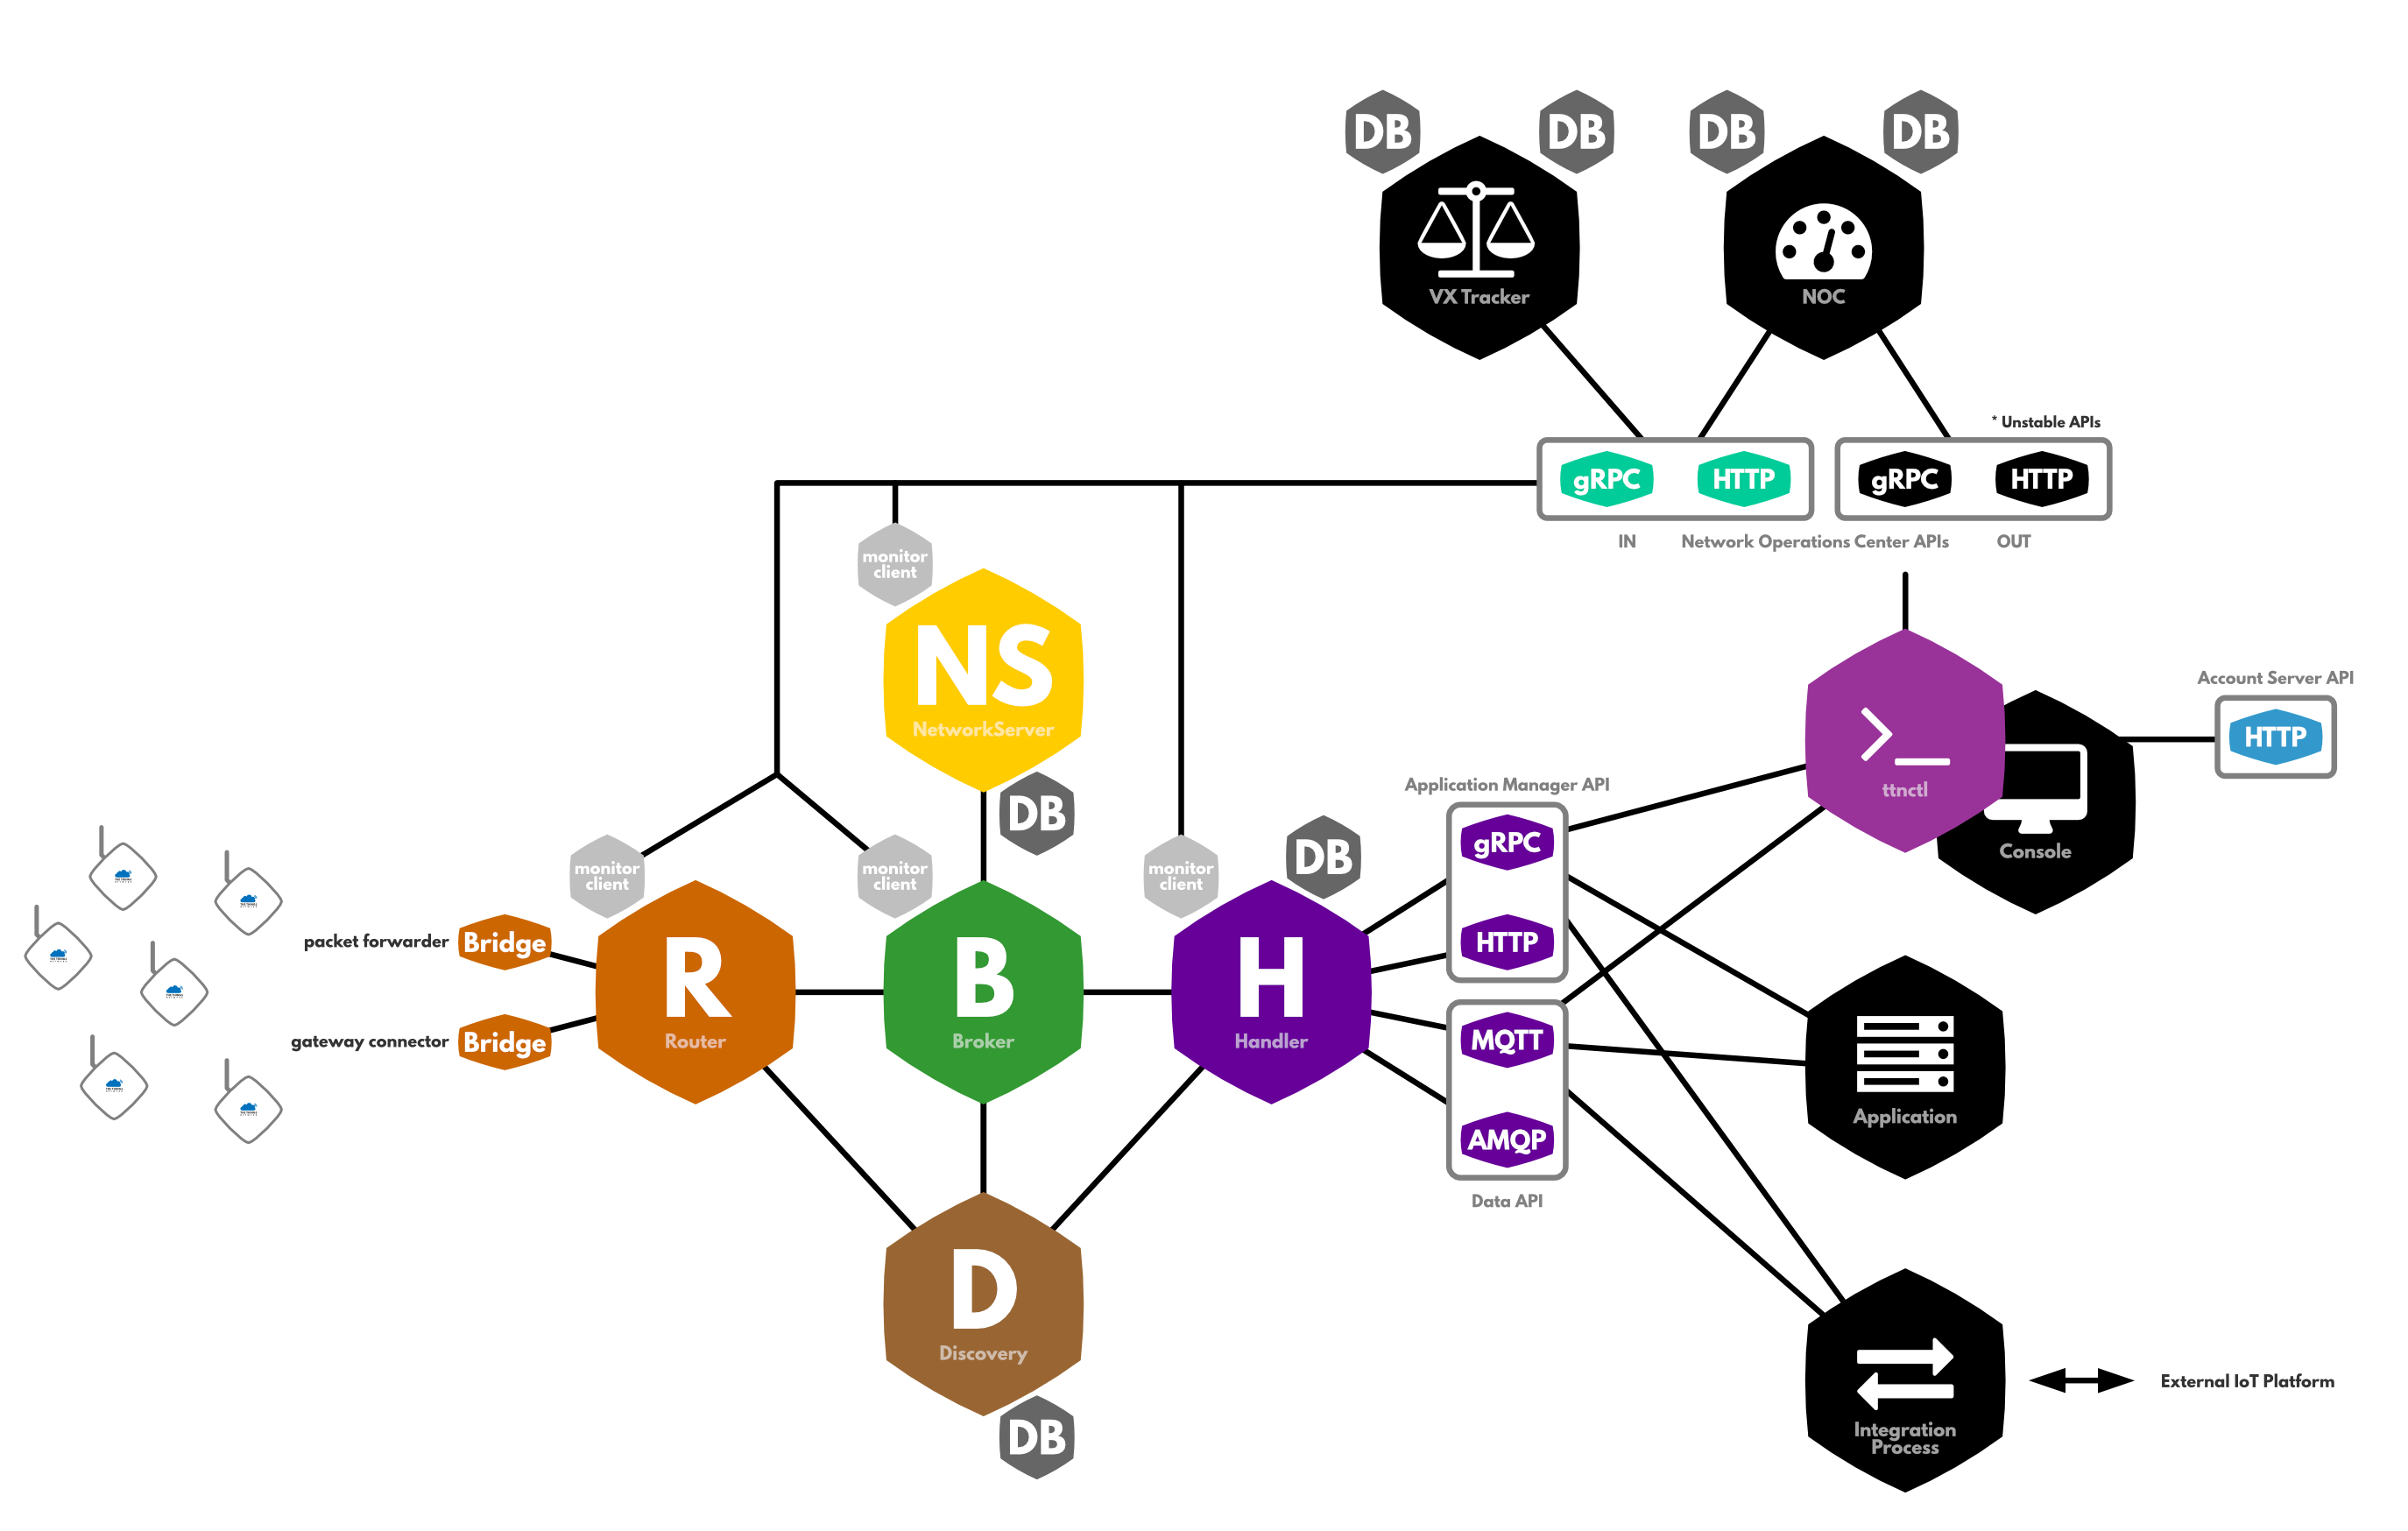
\includegraphics[width=\textwidth]{img/ttn/ttn_architecture.png}
	\caption[TTN Architektur]
	{TTN Architektur, Quelle: TTN Webseite - Home \cite{ttnhome}}
\end{figure}

\newpage
\noindent
In dieser Arbeit wird \textbf{nicht auf die Details des TTN Netzwerkes eingegangen}. Wie das System in sich funktioniert hat keinen Einfluss auf das ATAS Projekt. Das TTN Netzwerk wird als Blackbox betrachtet. Die untenstehende Grafik verbildlicht diesen Ansatz. Über das TTN Netzwerk, via Gateways (G), werden Daten an die Tracker (N) gesendet. Die Tracker senden Ihre Daten via Gateway an das TTN. Das TTN Netzwerk wiederum bietet Schnittstellen an (API) um Daten zu senden und zu empfangen.

\begin{figure}[H]
	\centering
	\includegraphics[width=\textwidth]{img/ttn/ttn-overview.jpg}
	\caption[TTN Blackbox]
	{TTN Blackbox, Quelle: TTN Webseite \cite{ttnwiki}}
\end{figure}
\noindent

\subsection{Datenschnittstelle / API}
Durch die Wahl von TTN als LoRaWan Netzwerk muss die Datenübertragungsart MQTT genutzt. Der Zugriff auf die Datenschnittstelle (API) von TTN ist nur per MQTT möglich. Die Unterstützung von AMQP ist geplant aber noch nicht verfügbar \cite{amqp}. Das Protokoll MQTT war dem Projektteam bereits bekannt. Während dem Studium konnten bereits positive Erfahrungen mit MQTT gesammelt werden.

\chapter{Systembeschreibung - Detail}
Die vorhergegangene Architekturbeschreibung gibt einen grobe ersten Überblick über das System. Technische Details zu  den verwendeten Technologien oder den genauen Fluss der Kommunikation waren nicht ersichtlich. In diesem Abschnitt soll nun intensiv auf diese Thematik eingegangen werden.\\[0.3cm]
Auf der nachfolgenden Seite finden Sie ein Schema welches einen genauen Überblick über das System liefert.\\[0.3cm]
Die Komponenten werden in 2 Kategorien eingeteilt. Komponenten mit einem blauen Box wurden im Rahmen dieser Arbeit selbständig erarbeitet. Um einen möglichst guten und kompletten Überblick über das System zu liefern, wird nicht zwischen Hard und Software unterschieden. Gelbe Wolken markieren einen Internetservice welcher für den Aufbau des Systems integriert wurde. Blaue Zylinder markieren eine Datenbanklösung. Das Abbild einer Person markiert einen User des Systems.

\begin{figure}[H]
	\centering
	\includegraphics[width=0.45\textwidth]{img/system/legend.jpg}
	\caption[Legende - Diagram]
	{Legende - Diagram}
\end{figure}

\noindent
Die im Absatz beschriebene Komponente wird als graue Box dargestellt und so hervorgehoben.
\begin{figure}[H]
	\centering
	\includegraphics[width=0.45\textwidth]{img/system/greybox.jpg}
	\caption[Legende - Diagram - graue Box]
	{Legende - Diagram - graue Box}
\end{figure}

\newpage
\section{Überblick}
\begin{figure}[H]
	\centering
	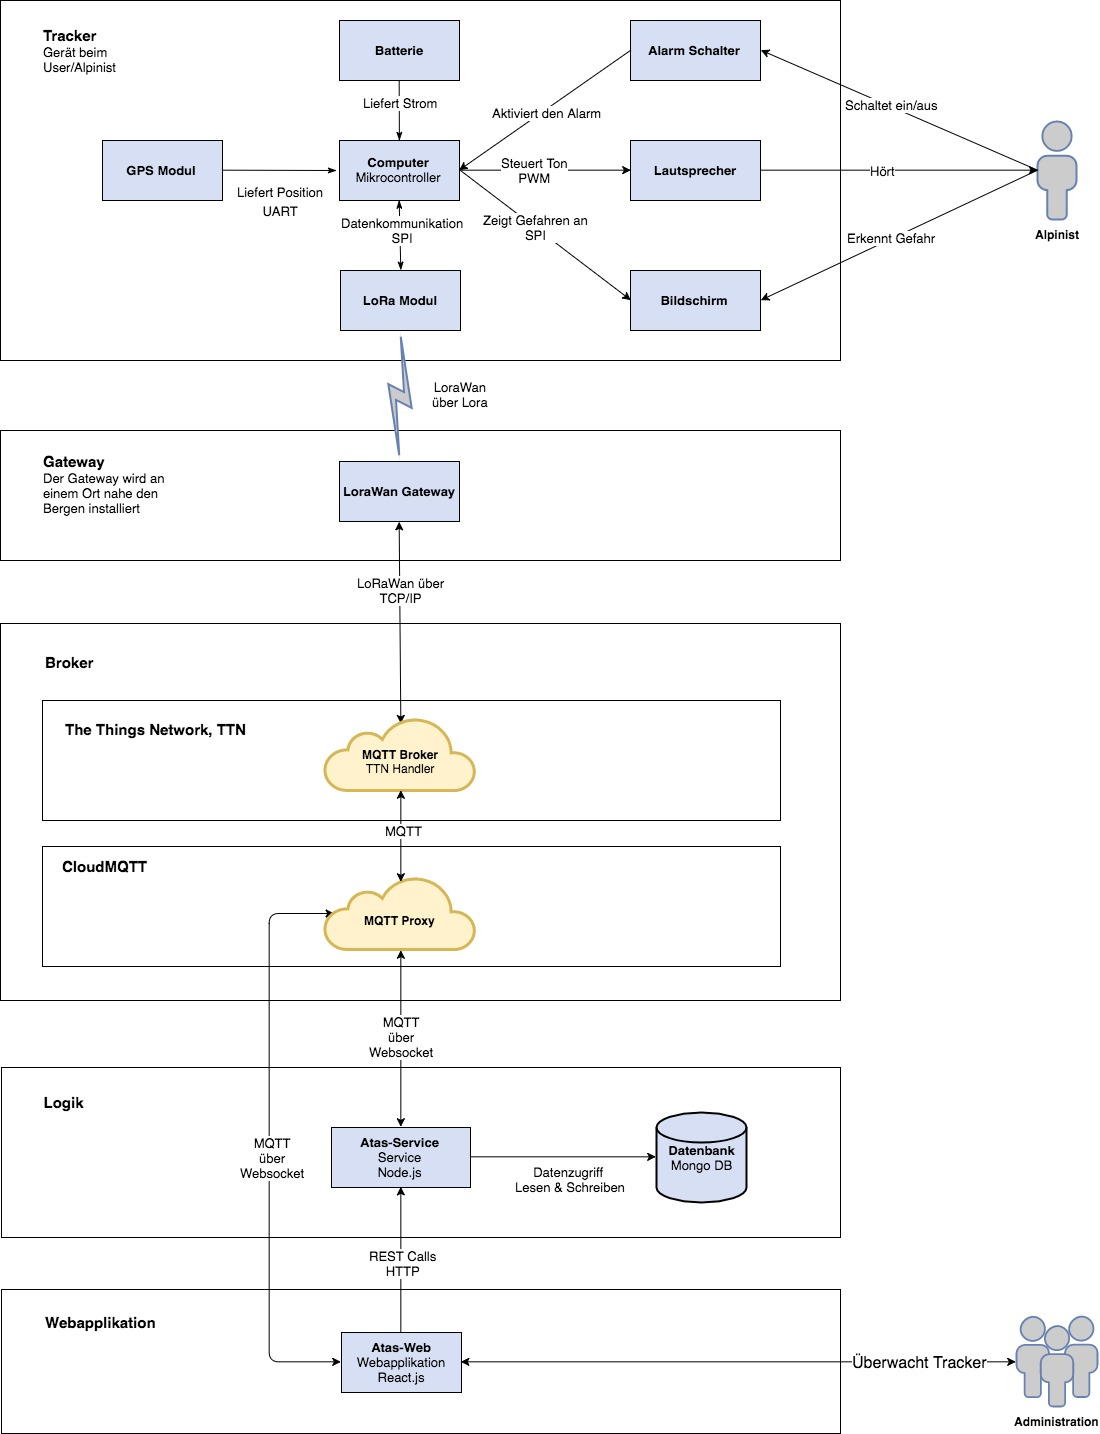
\includegraphics[width=0.95\textwidth]{img/system/ATAS_SystemOverview_Detail_BA.jpg}
	\caption[Systemübersicht Detail]
	{Systemübersicht Detail}
\end{figure}

\newpage
\section{Tracker}
Wie in der untenstehenden Grafik ersichtlich, besteht der Tracker aus mehreren Komponenten/Modulen. Welche Komponenten verbaut und wie diese untereinander kommunizieren, wird im Kapitel 'Prototyp' genauer behandelt.
\begin{figure}[H]
	\centering
	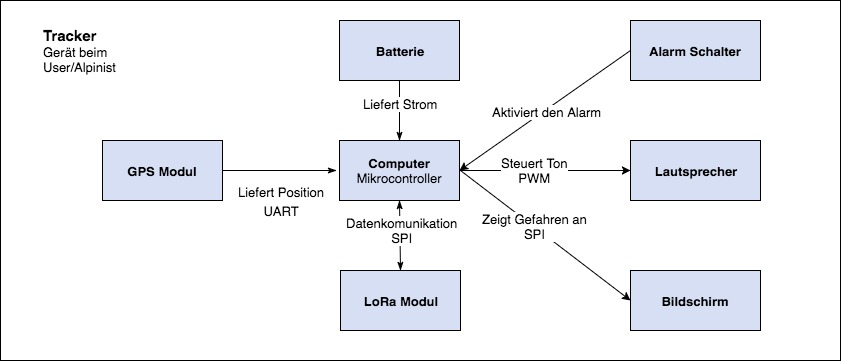
\includegraphics[width=\textwidth]{img/system/ATAS_SystemOverview_Tracker_BA.jpg}
	\caption[Tracker Detail]
	{Tracker Detail}
\end{figure}

\begin{itemize}
	\item
	Alarm Schalter: Mit dem Druck auf den Knopf können die Überwacher über eine Notsituation aufmerksam gemacht werden. Bspw. Wenn der Alpinist einen Unfall hatte und nun bewegungsunfähig ist.
	\item
	Lautsprecher: Über den Lautsprecher kann der Alpinist über eine Gefahrenquelle mit einem akustischen Signal aufmerksam gemacht werden. Bspw. Wenn sich der Alpinist in einem Bereich am Berg mit erhöhter Gefahr für Lawinen aufhält. Der Lautsprecher dient zur Information, \textbf{dass ein Problem besteht}.
	\item
	Display: Über ein Display können mehr Informationen zum Tracker und den Gefahrenzonen angezeigt werden. Das Display dient zur Information, \textbf{was für ein Problem besteht}.
	\item
	GPS Modul: Der Tracker verfügt über ein GPS Modul. Mit dem GPS Modul kann die Position des Tracker auf der Erde ermittelt werden.
	\item 
	Lora Modul: Mittels Lora Modul können Daten an einen Empfänger (LoRaWan Gateway) gesendet werden.
	\item 
	Computer: Verarbeitet eingehenden Signale und löst entsprechende Aktionen aus.
\end{itemize}

\newpage
\subsection{ATAS-Node}
ATAS-Node ist die Software welche auf dem Tracker Gerät ausgeführt wird. ATAS-Node wurde, im Vergleich zum Vorprojekt, komplett umgebaut. Genauere Angaben, die ATAS-Node aufgebaut wurde ist im Abschnitt Prototype zu finden.2

\newpage
\section{Gateway}
Der Gateway verbindet die Tracker mit dem \gls{TTN} Netzwerk. Er sendet Daten zu den Trackern (\gls{Downlink}) und empfängt Daten von den Trackern (\gls{Uplink}).
\subsection{Diagramm}
\begin{figure}[H]
	\centering
	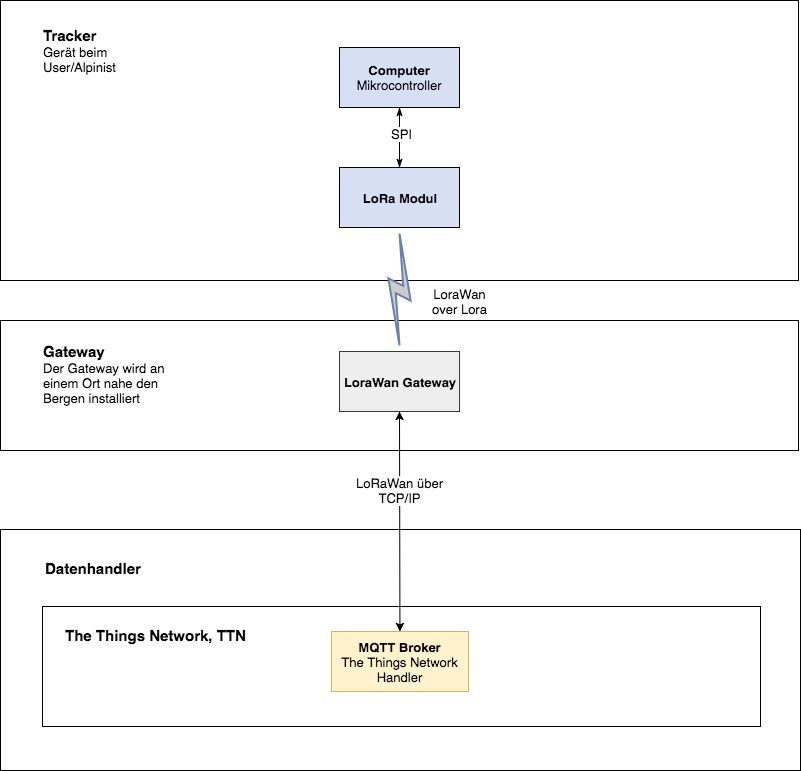
\includegraphics[width=\textwidth]{img/system/ATAS_SystemOverview_Detail_Gateway_BA.jpg}
	\caption[Gateway Detail]
	{Gateway Detail}
\end{figure}

\newpage
\section{Datenhandler}
Die Aufgabe des Datenhandlers umfasst das Sammeln der Daten und deren Bereitstellung an die ATAS Applikationen ATAS-Web und ATAS-Service. Der Datenhandler besteht aus zwei Komponenten. Die Komponenten wurde nicht selbstständig entwickelt. Für das ATAS Projekt wurden bereits existierende Dienste verwendet. Die Dienste heissen \textbf{The Things Network (TTN)} und \textbf{CloudMQTT}. Was genau für Funktionen die einzelnen Dienste bieten wird in den nachfolgenden Abschnitten erklärt.

\subsection{The Things Network (TTN)}
TTN sendet Daten via Gateways an die Tracker. Über die Gateways empfängt das TTN Daten von den Trackern. Das TTN bietet einen Schnittstelle (MQTT Broker) um auf die Daten zuzugreifen.\\[0.3cm]
\textbf{Diagramm}
\begin{figure}[H]
	\centering
	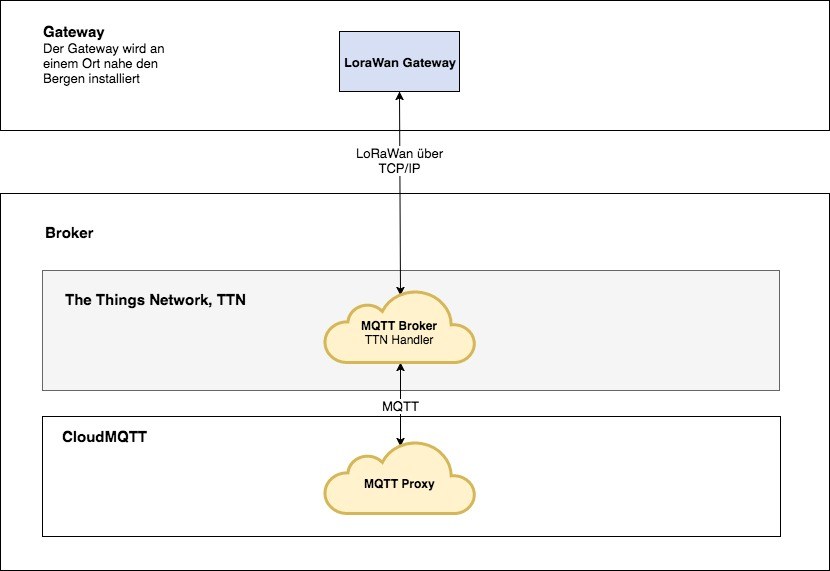
\includegraphics[width=\textwidth]{img/system/ATAS_SystemOverview_TTN_BA.jpg}
	\caption[TTN Detail]
	{TTN Detail}
\end{figure}

\newpage
\subsection{CloudMQTT}
Der MQTT Broker des TTN Netzwerkes bietet nur die Möglichkeiten die Daten via MQTT abzurufen. Ein Zugriff via MQTT über Websockets wird nicht unterstützt. Im Internet fand ich recht schnell den Service 'Cloud' MQTT.   CloudMQTT spiegelt den TTN MQTT Broker, bietet aber zusätzlich ein Websocket Interface. ATAS-Web und ATAS-Service können nun via CloudMQTT Daten an die Tracker senden und empfangen.\\[0.3cm]
Alle Daten welche zu CloudMQTT publiziert werden, werden nun auch automatisch zum TTN MQTT Broker publiziert (Published). Alle MQTT Topics welche vom CloudMQTT abonniert werden, werden auch vom TTN MQTT Broker abonniert (Subscribe).  \\[0.3cm]
\textbf{Diagramm}
\begin{figure}[H]
	\centering
	\includegraphics[width=0.9\textwidth]{img/system/ATAS_SystemOverview_CloudMQTT_BA.jpg}
	\caption[TTN Detail]
	{TTN Detail}
\end{figure}

\newpage
\section{Logik}
\subsection{ATAS-Service}
Der ATAS-Service verwaltet die erfassten Gefahrenzonen. Er empfängt die Geo-Koordinaten der Tracker und vergleicht diese mit dem Koordinaten der Gefahrenzone. Wenn sich ein Tracker in einer Gefahrenzone befindet, wird ein Alarmsignal an den Tracker gesendet. Das Signal wird mittels MQTT an CloudMQTT gesandt. Das TTN Netzwerk wird informiert und übernimmt die Zustellung der Nachricht an den Tracker.\\[0.3cm]
ATAS-Service bietet unter anderem eine REST Schnittstelle an. Informationen zu den Gefahrenzonen können so von der WebApplikation (ATAS-Web) bezogen und gespeichert werden. Um die Datenbank zu speichern wurde eine MongoDB installiert und konfiguriert.\\[0.3cm]
ATAS-Service selbst ist eine node.js Applikation. Die verwendete Programmiersprache ist Javascript.
\begin{figure}[H]
	\centering
	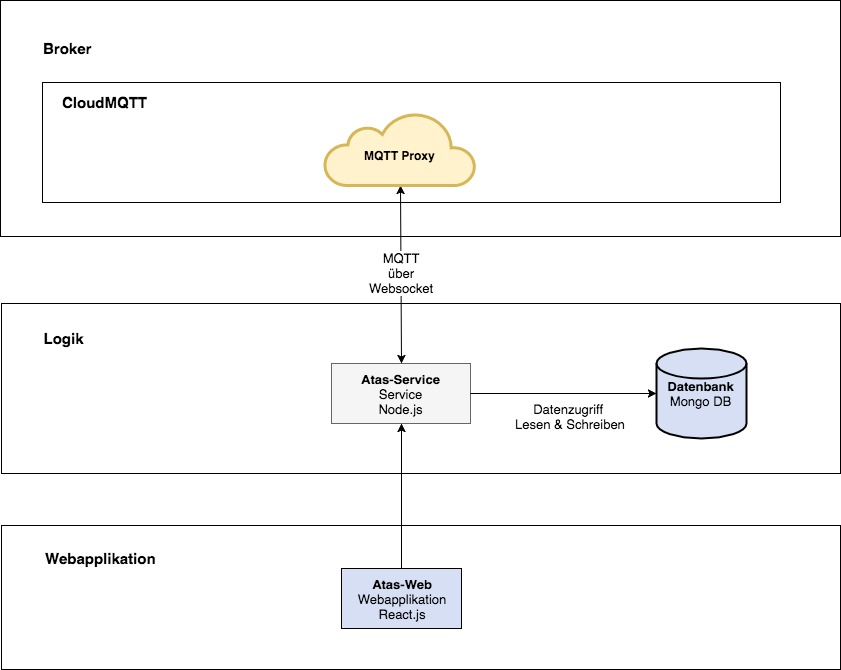
\includegraphics[width=\textwidth]{img/system/ATAS_SystemOverview_ATASService.jpg}
	\caption[ATAS-Service Diagram]
	{ATAS-Service Diagram}
\end{figure}
\newpage

\section{Webapplikation}
\subsection{ATAS-Web}
ATAS-Web ist eine Webapplikation. Die Applikation wurde mit der Programmiersprache Javascript realisiert. Um die Entwicklung zu beschleunigen wurde auf die Javascript React.Js zurückgegriffen. ATAS-Web bildet im wesentlichen das Management Interface für die Rettungsdienste. Über die Applikation kann die aktuelle Position der Tracker auf einer Karte dargestellt werden. Für die Kartendarstellung wurde Google Maps integriert.
\begin{figure}[H]
	\centering
	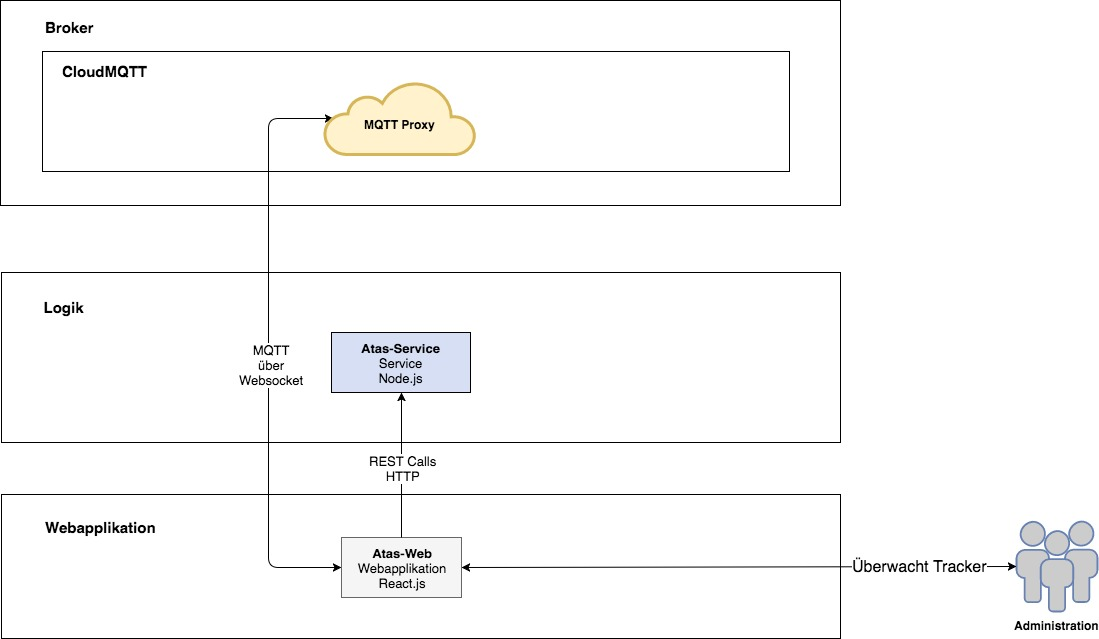
\includegraphics[width=\textwidth]{img/system/ATAS_SystemOverview_ATASWeb.jpg}
	\caption[ATAS-Web Diagramm]
	{ATAS-Web Diagramm}
\end{figure}

\newpage
\subsection{Übersicht}
Die nachfolgenden Bilder sollen aufzeigen wie ATAS-Web aussieht und wie dieses zu verwenden ist.

\subsubsection{Startseite}
Die Startseite der Applikation.
\begin{figure}[H]
	\centering
	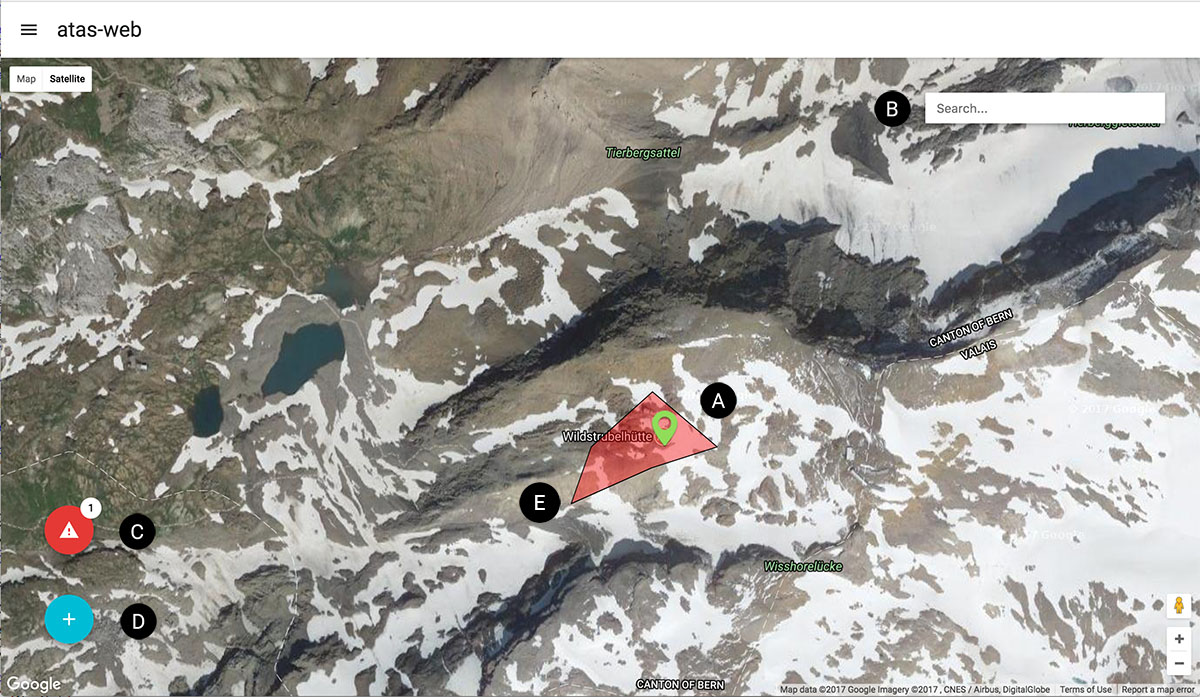
\includegraphics[width=\textwidth]{img/atasweb/atas-web.jpg}
	\caption[Startseite]
	{Startseite}
\end{figure}
Die Ansicht besteht aus verschiedenen Komponenten:
\begin{itemize}
	\item A: Auf der Karte wird die Position der Tracker dargestellt. 
	\item B: Suche nach Orten
	\item C: Anzeige der Tracker in Notsituationen
	\item D: Manuelles hinzufügen von Gefahrenzonen
	\item E: Gefahrenzone
\end{itemize}

\newpage
\subsubsection{Tracker}
Wird ein Tracker ausgewählt öffnet sich ein weiteres Menü.  Hier ersichtlich sind nebst der Tracker ID auch die genauen GPS Koordinaten. Über einen Alarmknopf kann ein Alarm auf dem Tracker ausgelöst werden.
\begin{figure}[H]
	\centering
	\begin{subfigure}{.45\textwidth}
		\centering
		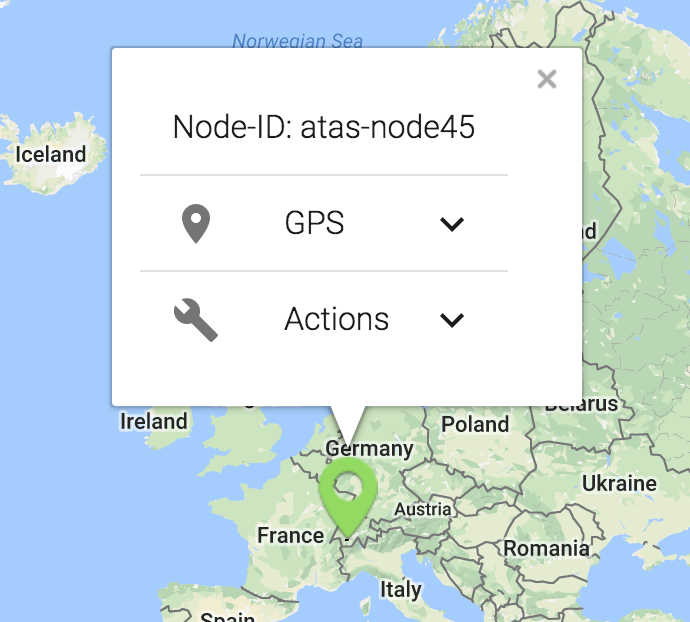
\includegraphics[width=0.9\textwidth]{img/atasweb/atas-web-node-closed.png}
		\caption[Tracker - Geschlossenes Menu]
		{Tracker - Geschlossenes Menu}
	\end{subfigure}%
	\begin{subfigure}{.45\textwidth}
		\centering
		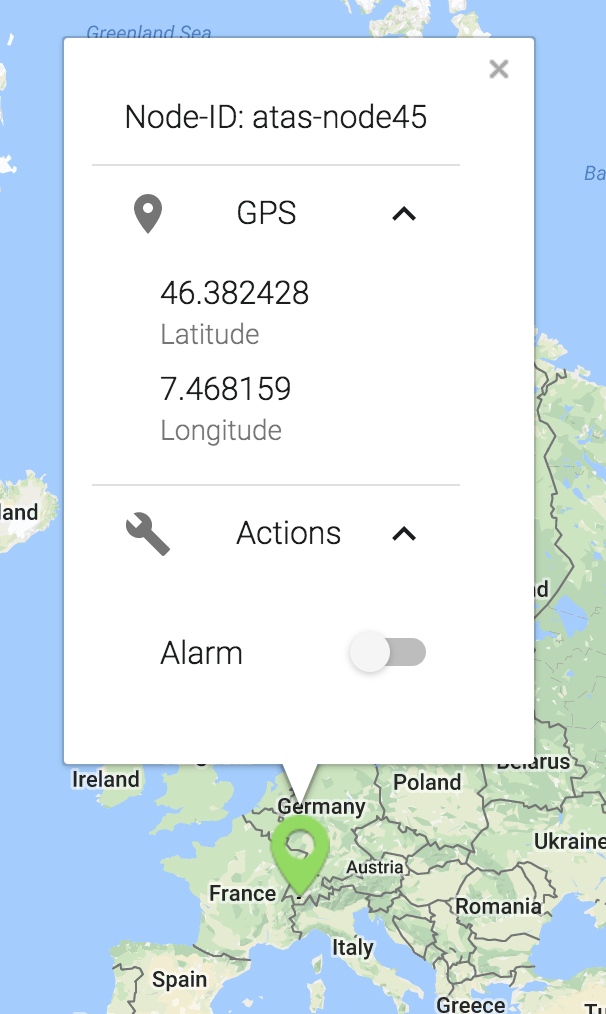
\includegraphics[width=0.7\textwidth]{img/atasweb/atas-web-node-open.png}
		\caption[Tracker - offenes Menu]
		{Tracker - offenes Menu}
	\end{subfigure}%
\end{figure}

\subsubsection{Alarmierung}
Über den roten Knopf kann eine neue Ansicht geöffnet werden. Die Ansicht gibt uns eine Übersicht über die Tracker, die sich in einer Gefahrenzone aufhalten oder den manuellen Alarm ausgelöst haben.
\begin{figure}[H]
	\centering
	\begin{subfigure}{.3\textwidth}
		\centering
		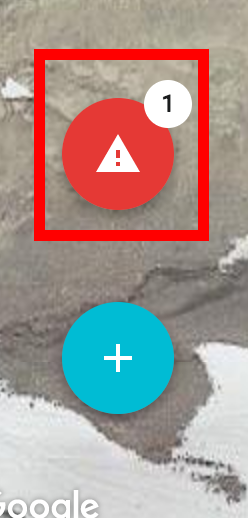
\includegraphics[width=0.4\textwidth]{img/atasweb/atas-web-alertbutton.png}
		\caption[Knopf zum öffnen der Alarmansicht]
		{Öffnet die Alarmansicht}
	\end{subfigure}%
	\begin{subfigure}{.65\textwidth}
		\centering
		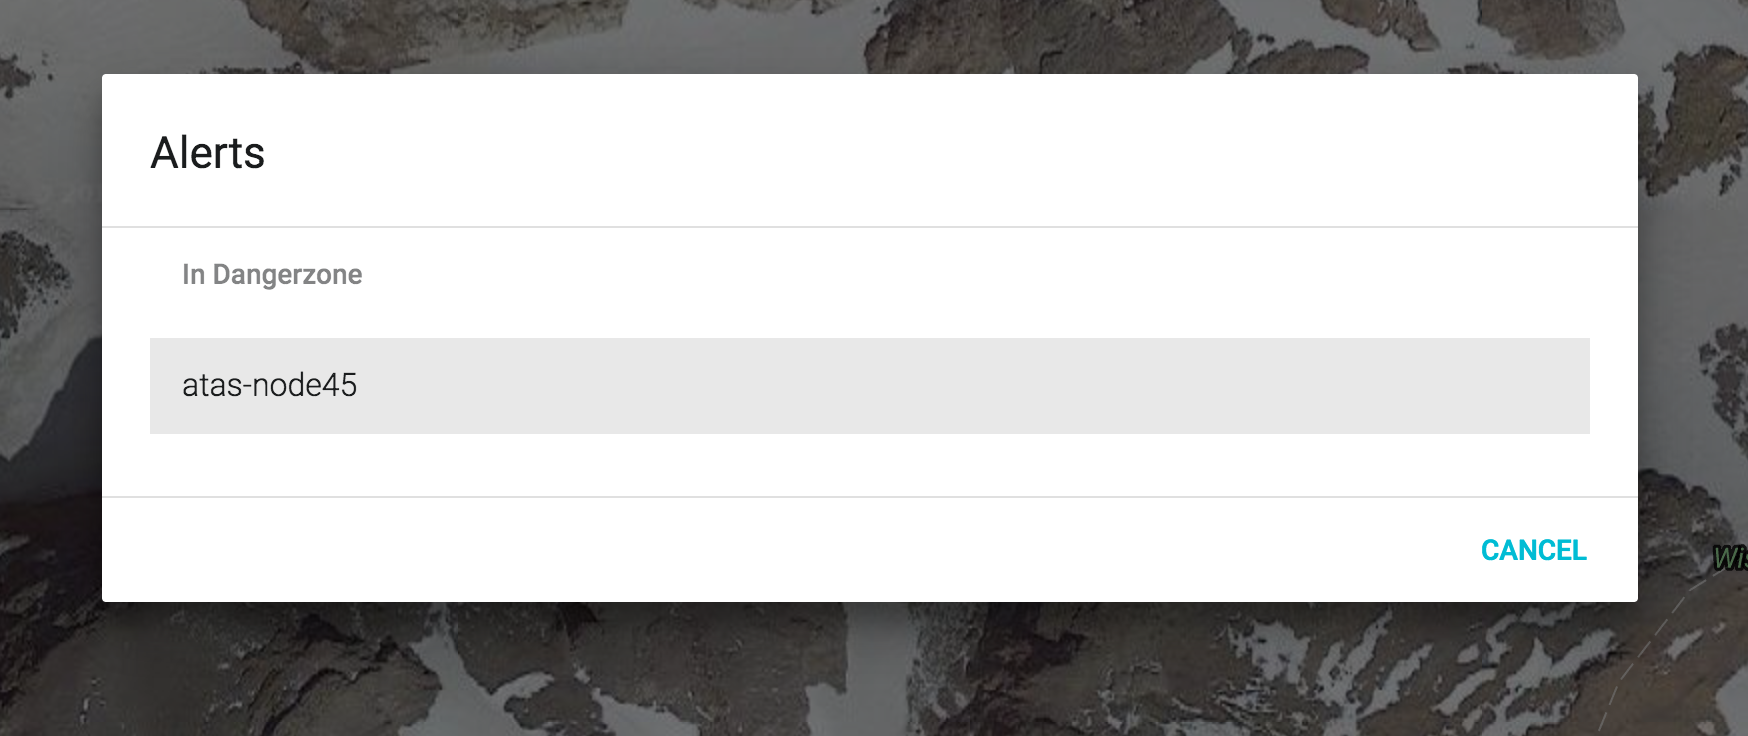
\includegraphics[width=0.9\textwidth]{img/atasweb/atas-web-alertoverview.png}
		\caption[Übersicht Alarme]
		{Übersicht Alarme}
	\end{subfigure}%
\end{figure}

\newpage 
\subsubsection{Gefahrenzonen}
Über den grünen Knopf können manuell Gefahrenzonen angelegt werden. Mittels 'Malwerkzeug' kann eine Polygon gezeichnet werden. Die entstandene Fläche repräsentiert eine Gefahrenzone.
\begin{figure}[H]
	\centering
	\begin{subfigure}{.2\textwidth}
		\centering
		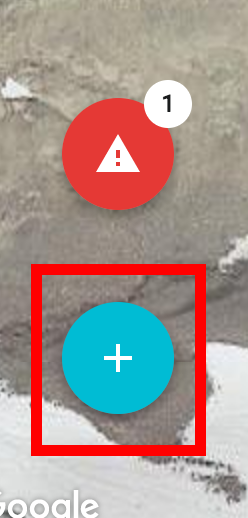
\includegraphics[width=0.9\textwidth]{img/atasweb/atas-web-addDangerzone.png}
		\caption[Knopf zum hinzufügen von Gefahrenzonen]
		{Hinzufügen Gefahrenzone}
	\end{subfigure}%
	\begin{subfigure}{.6\textwidth}
		\centering
		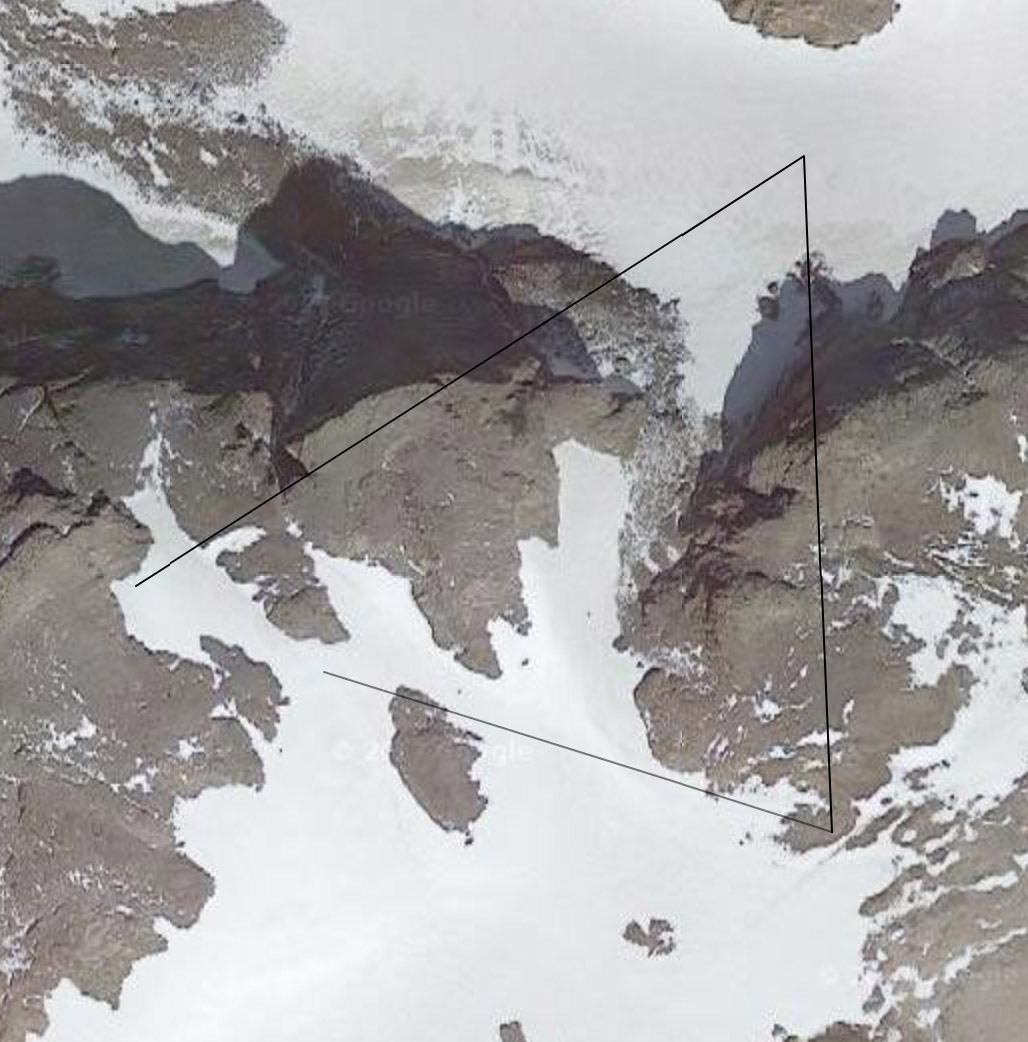
\includegraphics[width=0.65\textwidth]{img/atasweb/atas-web-drawing.jpg}
		\caption[Neue Zone zeichnen]
		{Neue Zone}
	\end{subfigure}%
\end{figure}
\begin{figure}[H]
	\centering
	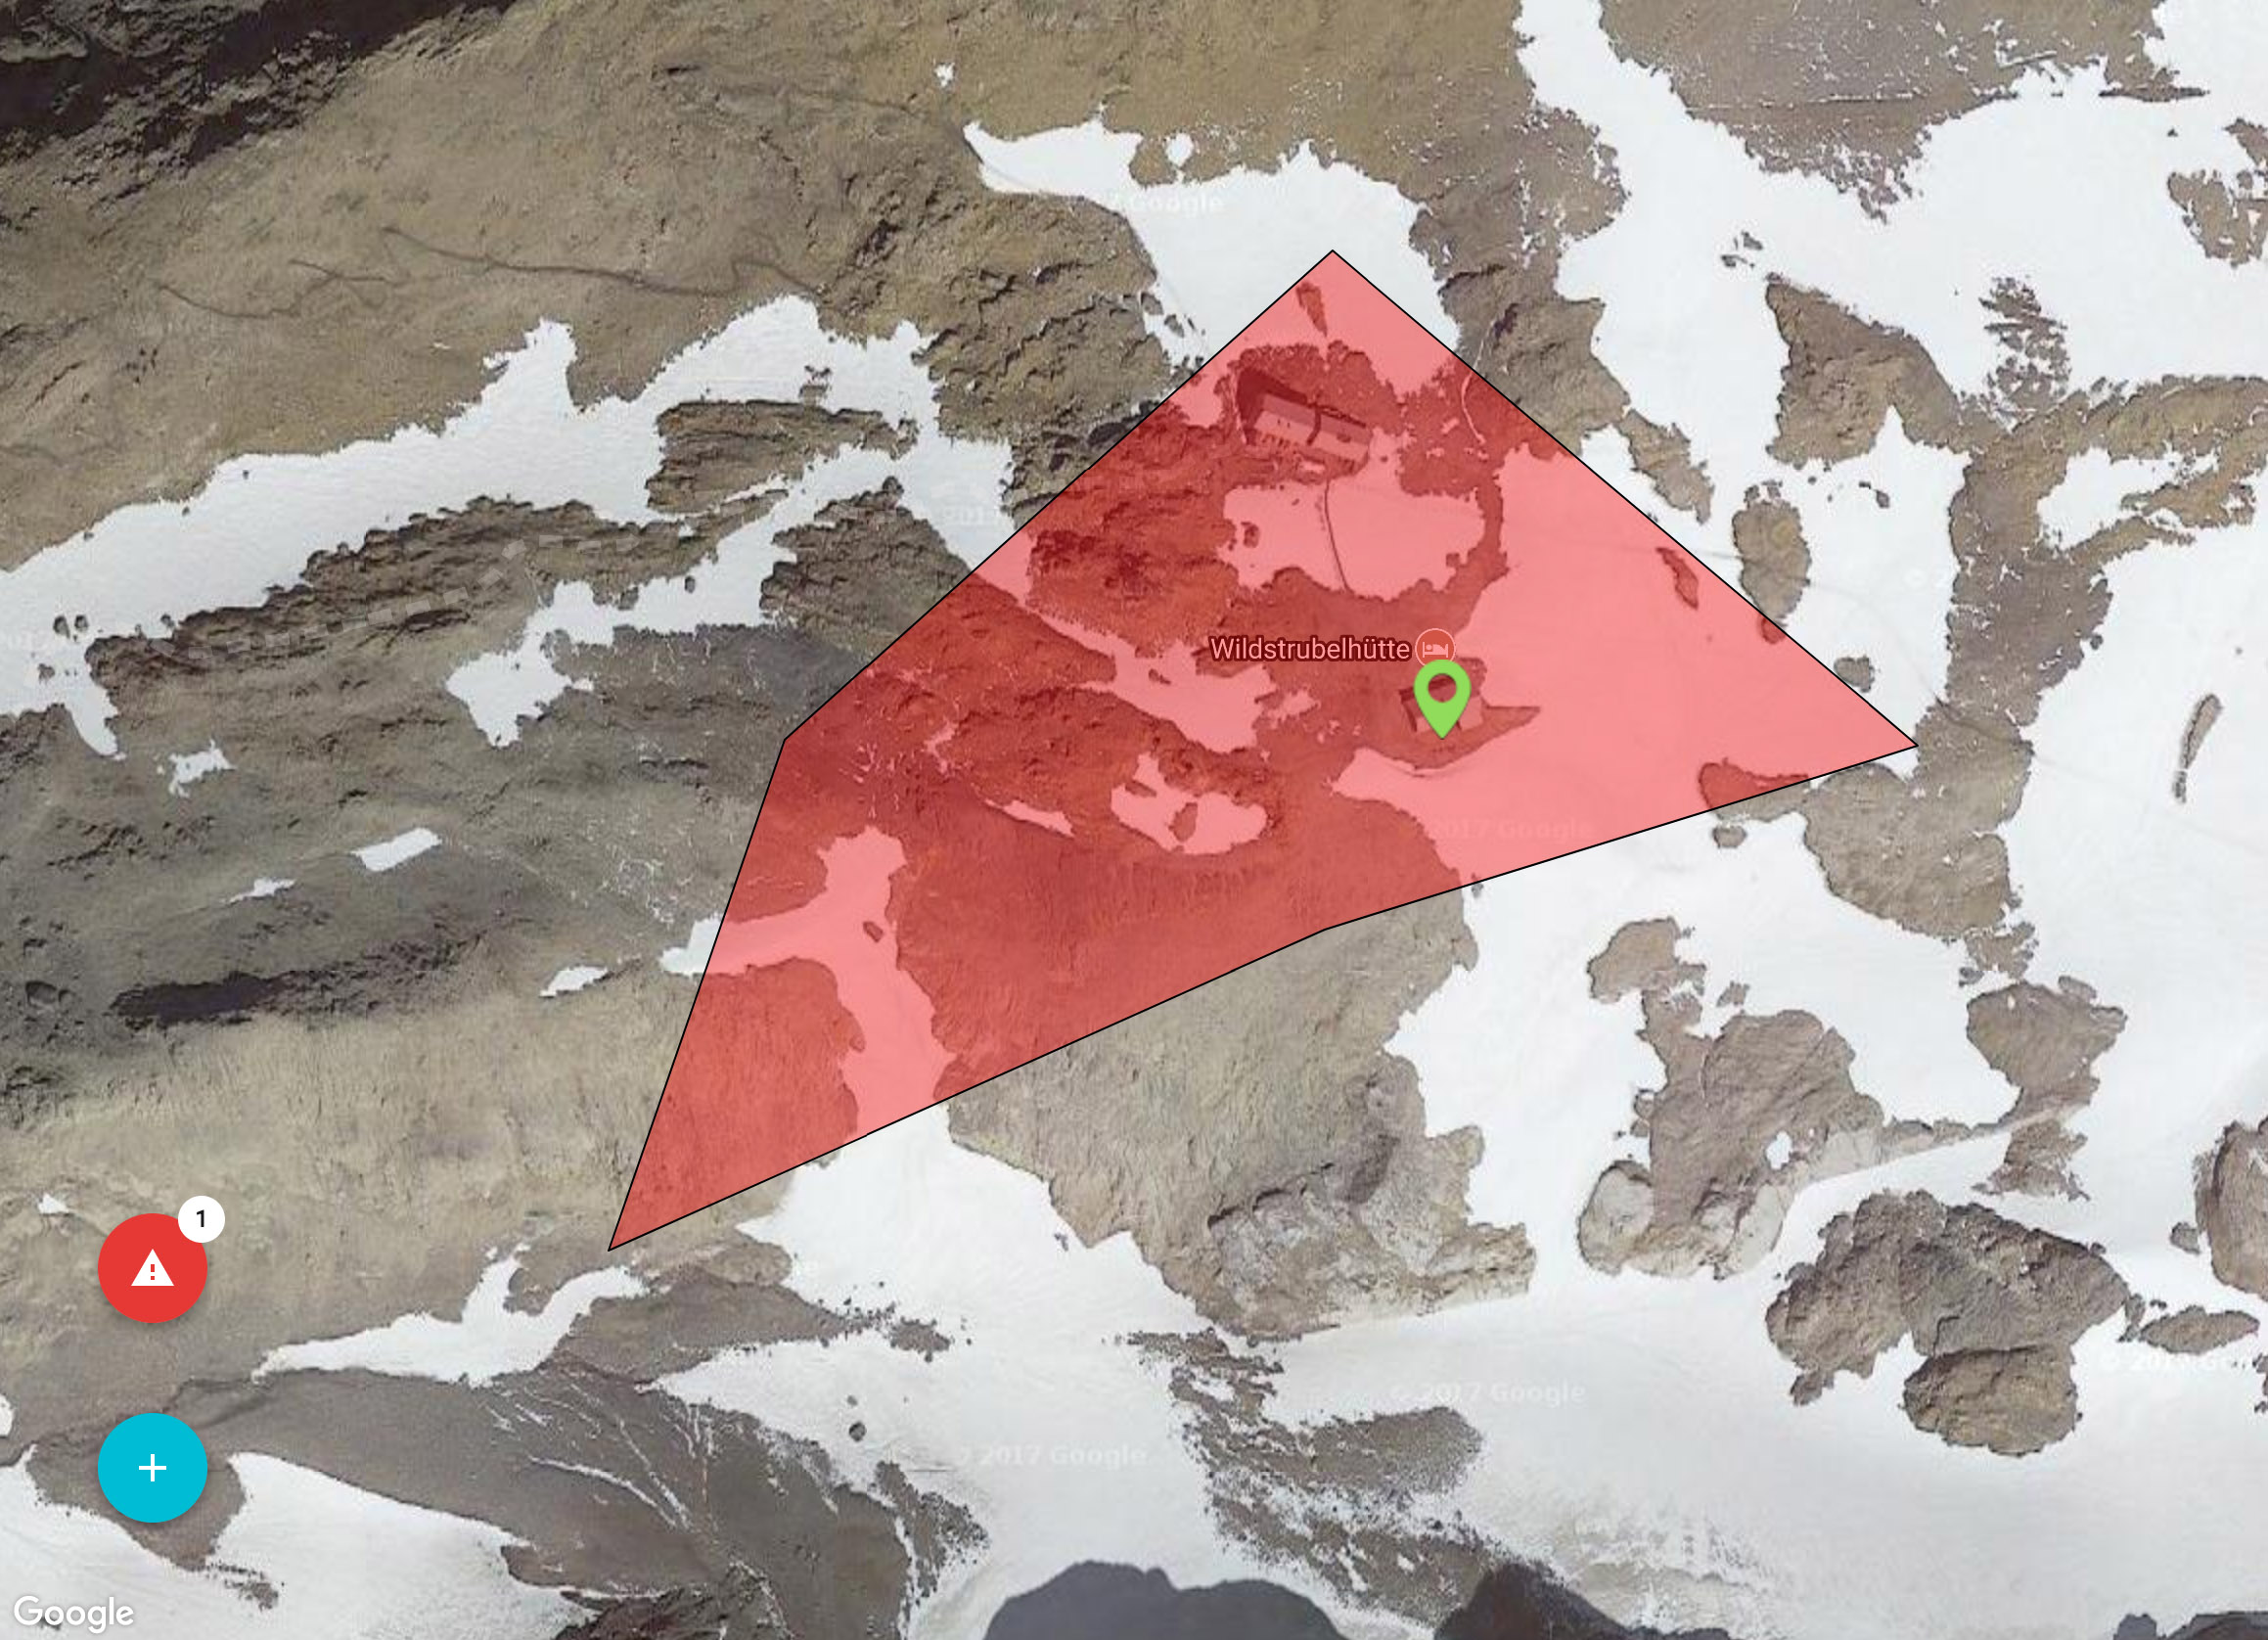
\includegraphics[width=0.8\textwidth]{img/atasweb/atas-web-dangerzone.jpg}
	\caption[Gefahrenzone]
	{Gefahrenzone}
\end{figure}%

\section{Daten Kommunikation}
In diesem Abschnitt wird die Daten Kommunikation zwischen den Komponenten im System aufgezeigt.
\subsection{MQTT}
Für das ATAS Projekt wurde die nachfolgende MQTT Struktur verwendet. Als MQTT Broker dient der MQTT Handler des TTN Netzwerkes resp. der MQTT Broker von CloudMQTT.
\begin{figure}[H]
	\centering
	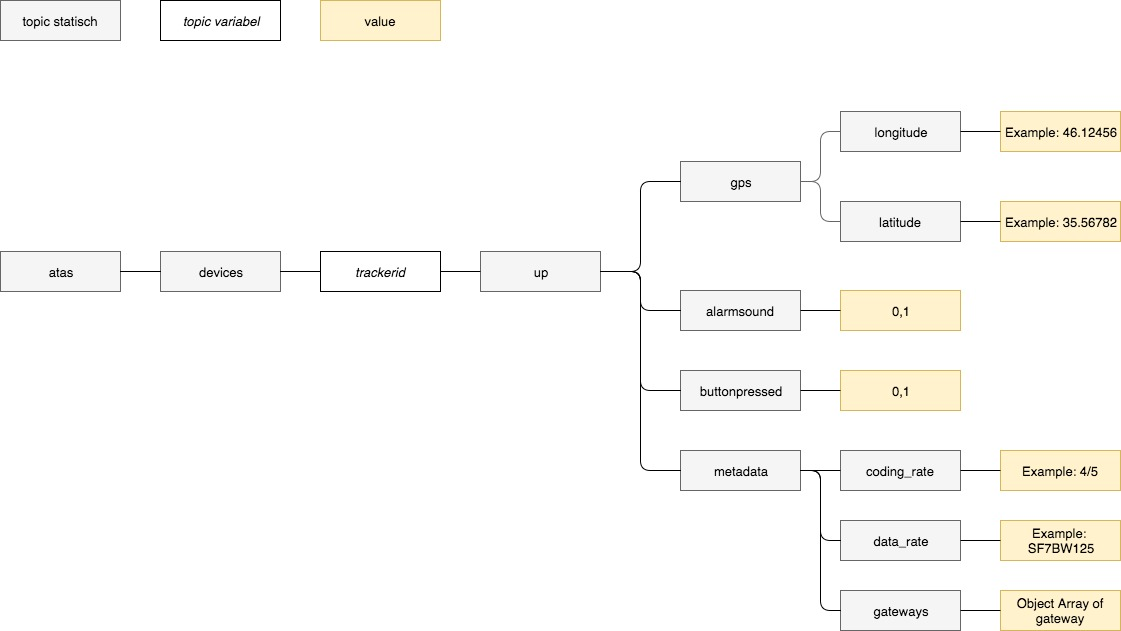
\includegraphics[width=\textwidth]{img/system/ATAS_MQTT_Topic_BA.jpg}
	\caption[MQTT Struktur]
	{MQTT Struktur}
\end{figure}

\subsection{Datenfluss Tracker TTN}
In diesem Abschnitt wird die Kommunikation zwischen Tracker und TTN Netzwerk genauer erläutert.\\[0.3cm]
Die Verbindung sieht wie folgt aus:
\begin{figure}[H]
	\centering
	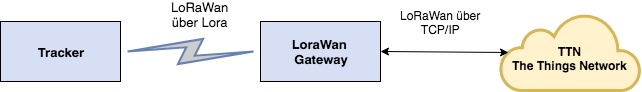
\includegraphics[width=\textwidth]{img/system/dataflow_tracker2ttn_connection.jpg}
	\caption[Verbindungen Tracker \& TTN]
	{Verbindungen Tracker \& TTN}
\end{figure}

\subsubsection{Uplink: Tracker zu TTN}
Der Tracker sendet in einem Uplink, 4 verschiedene Informationen:
\begin{itemize}
	\item Breitengrad, Geo-Koordinate, auf 5 Dezimalstellen genau
	\item Längengrad, Geo-Korrdinate, auf 5 Dezimalstellen genau
	\item Notfallknopf Status, Eingeschalten oder Ausgeschaltet
	\item In Gefahrenzone, dient der Kontrolle ob der Tracker die Nachricht erhalten hat
\end{itemize}
Die maximale gösse des Uplinks beträgt \textbf{20 Bytes}. Diese Angabe wird später im Bereich 'Testing' benötigt.
\begin{figure}[H]
	\centering
	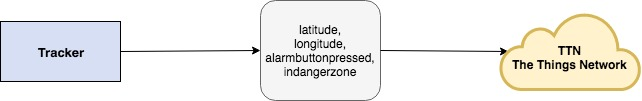
\includegraphics[width=\textwidth]{img/system/dataflow_tracker2ttn_uplink.jpg}
	\caption[Tracker Uplink]
	{Tracker Uplink}
\end{figure}

\subsubsection{Downlink: TTN zu Tracker}
Das TTN Netzwerk sendet die Information ob sich der Tracker in einer Gefahrenzone befindet. Der gesendete Wert signalisiert ebenfalls um was für eine Gefahr es sich handelt. 5 Werte sind dabei möglich
\begin{itemize}
	\item 0, keine Gefahr
	\item 1, Lawine
	\item 2, Steinschlag
	\item 3, Schneesturm
	\item 4, Spalten
\end{itemize}

\begin{figure}[H]
	\centering
	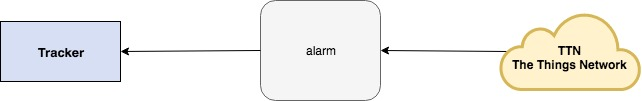
\includegraphics[width=\textwidth]{img/system/dataflow_tracker2ttn_downlink.jpg}
	\caption[Tracker Downlink]
	{Tracker Downlink}
\end{figure}
\chapter{Prototyp}
Die Bachelorarbeit wird in 2 Hauptaufgaben aufgeteilt.\textbf{ Testing} und das erstellen eines zweiten Prototyps nachfolgend genannt \textbf{Prototyp 2}. Dieses Kapitel beschreibt, wie beim Entwickeln des Prototypen 2 vorgegangen bin.

\section{Begründung neuer Prototyp}
Es gibt diverse Gründe für den Bau eines neuen Prototypen:
\begin{enumerate}
	\item Auf dem Prototyp 1 wird ein vollwertiges Betriebssystem (Raspian, Linux Derivat) eingesetzt. Einige Funktionen bspw. das Lesen der GPS Daten werden vom System sehr vereinfacht. Dies ermöglichte mir einen raschen und unkomplizierten Aufbau der Software. Obschon ein solches 'High Level' OS eine grosse Hilfe in der Entwicklung darstellt, ist es in der Industrialisierung der Lösung eher hinderlich. Der Einsatz eines OS hat diverse Nachteile
	\begin{itemize}
		\item Vom OS selbst benötigen wir für den Betrieb der ATAS-Node Software nur einen Bruchteil der Funktionalität. Speicher, Memory und Systemperformance wird für Systemprozesse verschwendet. 
		\item Durch die hohe Auslastung des Systems werden stärkere Prozessoren benötigt. Der Energieverbrauch der Lösung steigt.
		\item Mehr Software bedeutet zwangsläufig mehr Fehlerquellen. Obschon das eingesetzte System (Raspian) als Stabil gilt, kann es aufgrund der Softwarekomplexität zu Fehlern kommen.
		\item Durch den Einsatz eines OS reduzieren wir die Sicherheit des ganzen Systems. Je mehr Interfaces ein System anbietet, desto anfälliger wird es für den unerlaubten Zugriff.
	\end{itemize}
	\item Der Prototyp 1 bietet viele Anschlussmöglichkeiten. Bspw. für ein Display, USB, oder eine RJ45 Buchse. Funktionen welche die  Entwicklung stark vereinfachen, aber den Energieverbrauch erhöhen und die Grösse des Systems unnötig vergrössern. 
	\item Die Verbauten Komponenten sind nicht für eine Industrialisierte Lösung geeignet. Die Komponenten hindern das Projekt daran eine professionelle Form anzunehmen.
\end{enumerate}

\section{Ablauf Prototyping}
Aus meiner Sicht bildet der während der Arbeit zu konstruierende Prototyp 2 nur einen Zwischenschritt bis zu Finalen Version. Eine Visualisierung meiner Vorstellung:\\
\begin{figure}[H]
	\centering
	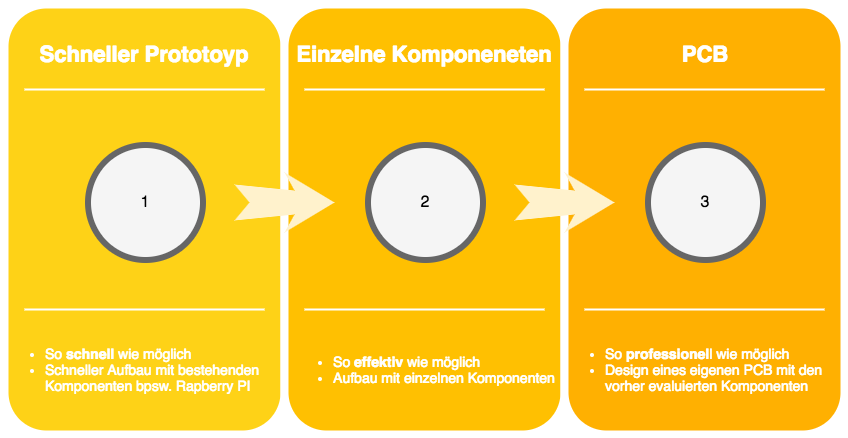
\includegraphics[width=\textwidth]{img/projectFlow_Prototype.png}
	\caption[Prototyping Ablauf]
	{Prototyping Ablauf}
\end{figure}
\noindent
Mein Ziel ist es mit dem Umstieg auf andere Komponenten, den Grundstein für den Prototypen 3 zu legen. Der Prototyp 3 ist nicht Bestandteil dieser Arbeit. Prototyp 3 bildet die finale Prototyp Version. Die Einzelnen Komponenten vom Prototyp 2 werden auf einen eigens designeten PCB installiert. Durch diesen Schritt würde sich das System in Sachen Platzbedarf nochmals massiv verbessern.

\newpage
\section{Ablauf Vorgehen}
Der im Projekt 2 erstellte Prototyp wurde mit sehr simplen vorgefertigten Elektronikkomponenten umgesetzt. Ziel dieser Arbeit war es in möglichst kurzer Zeit einen funktionsfähigen Prototypen aufzubauen. Während dieser Arbeit sollen nun neue Komponenten evaluiert und ein zweiter Prototyp erstellt werden. Der Ablauf dieser Phasen sieht wie folgt aus:\\[0.3cm]

\begin{figure}[H]
	\centering
	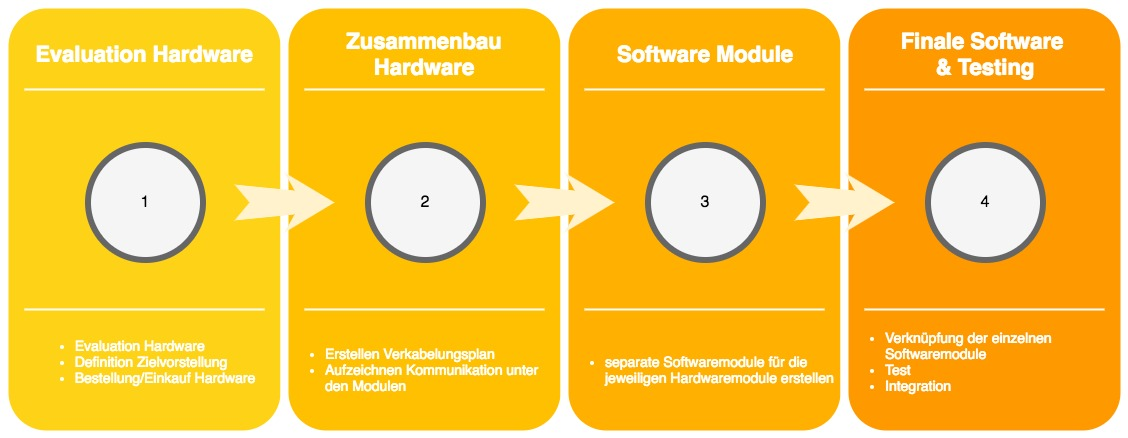
\includegraphics[width=\textwidth]{img/projectFlow_hardware.jpg}
	\caption[Flowchart Prototyp 2]
	{Ablauf für den Aufbau des zweiten Prototyps}
\end{figure}
\noindent
Die einzelnen Schritte werden auf den kommenden Seiten detailliert erklärt.

\newpage
\section{Evaluation Hardware}
Auf Grundlage der bestehenden Prototyps soll neue Hardware evaluiert werden. Der Funktionsumfang des Prototyps soll gleichwertig bleiben. Sind die Komponenten erst definiert, wird das Material bestellt.\\
Für den Aufbau des zweiten Prototypen wurde die nachfolgende Hardware verwendet.\\[0.5cm]
\begin{tabularx}{\linewidth}{XXX}
		\textbf{Gerätetyp} & \textbf{Model} & \textbf{Bild} \\ \hline
		Entwicklungsboard & \makecell[l]{Espressfif ESP-WROOM-32\\ Core Dev Kit}  & \parbox[c]{1em}{
			\vspace{8pt}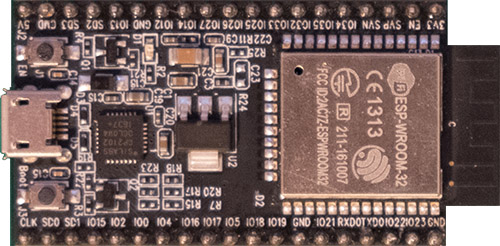
\includegraphics[width=0.3\textwidth]{img/prototype/esp32.jpg}\vspace{8pt}} \\ \hline
		GPS Module& ublox Neo 6M & \parbox[c]{1em}{
			\vspace{8pt}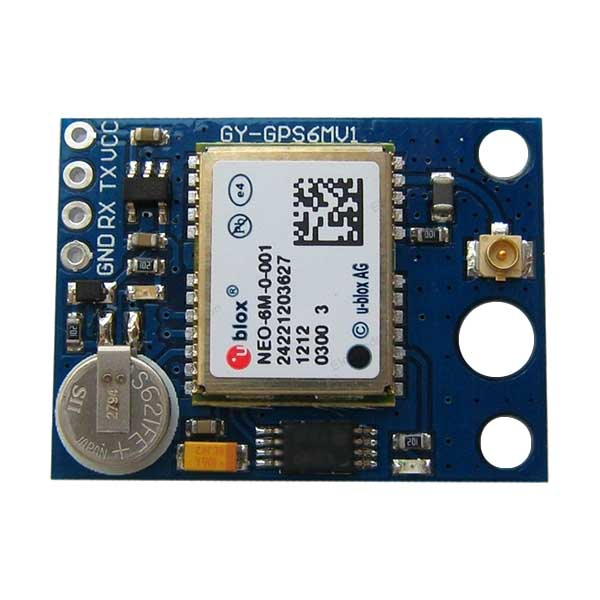
\includegraphics[width=0.3\textwidth]{img/prototype/gps.jpg}\vspace{8pt}} \\ \hline
		Lora Modul & RFM96 & \parbox[c]{1em}{
			\vspace{8pt}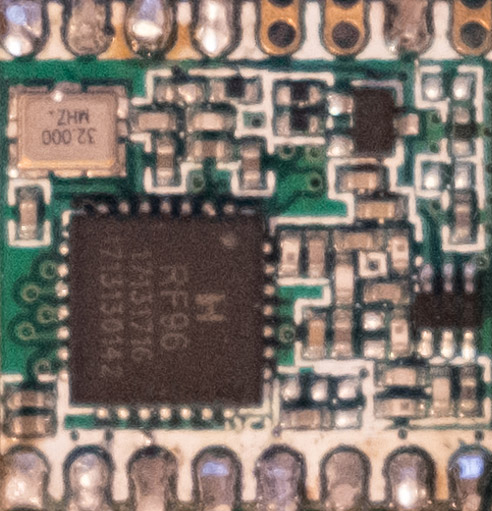
\includegraphics[width=0.18\textwidth]{img/prototype/lora.jpg}\vspace{8pt}} \\ \hline
		Speaker & Piezo Speaker  & \parbox[c]{1em}{
			\vspace{8pt}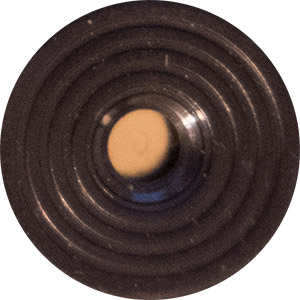
\includegraphics[width=0.15\textwidth]{img/prototype/speaker.jpg}\vspace{8pt}} \\ \hline
		Display & \makecell[l]{eink Display Waveshare \\ 1.54  Zoll 200x 200}  &\parbox[c]{1em}{
			\vspace{8pt}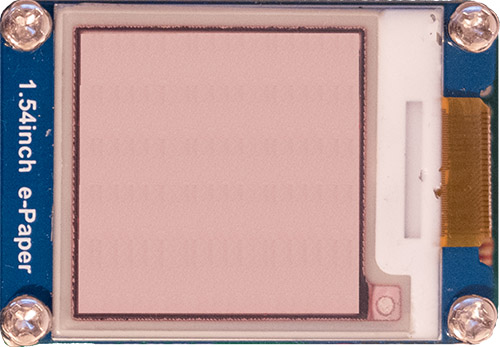
\includegraphics[width=0.3\textwidth]{img/prototype/display.jpg}\vspace{8pt}} \\ \hline
		Schalter & gewöhnlicher 4 Pin Schalter & \parbox[c]{1em}{
			\vspace{8pt}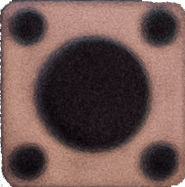
\includegraphics[width=0.07\textwidth]{img/prototype/schalter.png}\vspace{8pt}} \\ \hline
\end{tabularx} 
\noindent
Für die Komponenten gab es keine vorgegebenen Spezifikationen. Aus diesem Grund wurden diese nach Internetrecherchen und Empfehlungen von Mitstudierenden beschafft. 
\newpage
\subsection{Lora-Antenne}
Es wurde angenommen, dass beim Kauf des Lora-Moduls eine Antenne mitgeliefert wird. Leider war dies nicht der Fall. Dieser Zwischenfall stellte eine gute Gelegenheit dar, das Wissen über die Telekommunikationswelt zu vertiefen. Es wurde entschieden keine erneute Bestellung auszulösen und stattdessen  die Antenne einfach eigenhändig zu bauen. Nach einer kurzen Internetrecherche stellte sich heraus , dass mit simplen Komponenten eine zuverlässige Antenne für 868Mhz gebaut werden kann \cite{wavelengthTTN}. Ein einfaches Kabel ist ausreichend. Das Kabel muss die Länge der Wellenlänge oder einen Bruchteil bspw. 1/2 oder 1/4 der Wellenlänge haben. Die Berechnung der Wellenlänge ist mit der nachfolgenden Formel möglich \cite{wavelength}.\\[0.3cm]
Es gilt $\lambda$ = Wellenlänge, v = Übertragungsgeschwindigkeit (Lichtgeschwindigkeit), f = Durchschnitt der Frequenz (Lora Frequenz in Europa)
\begin{center}
	\begin{eqnarray*}
		\lambda &=& \frac{v}{f}\\
		\lambda &=& \frac{299.792.458 m/s}{868.000.000} = 34,54cm\\
		\frac{\lambda}{2} &=& \frac{34,53cm}{2} = 17,27cm\\
		\frac{\lambda}{4} &=& \frac{17,27cm}{2} = 8,63cm \\
	\end{eqnarray*}
\end{center}
17,27cm sind für den Prototypen zu lange. Es wurde entschieden, 1/4 der Wellenlänge zu verwenden. Für eine Antenne musste also nur ein Kabel mit der Länge \textbf{8.63cm} vorbereitet und mit dem Antennenport des Lora Moduls verbunden werden.
\newpage
Das Resultat:
\begin{figure}[H]
	\centering
	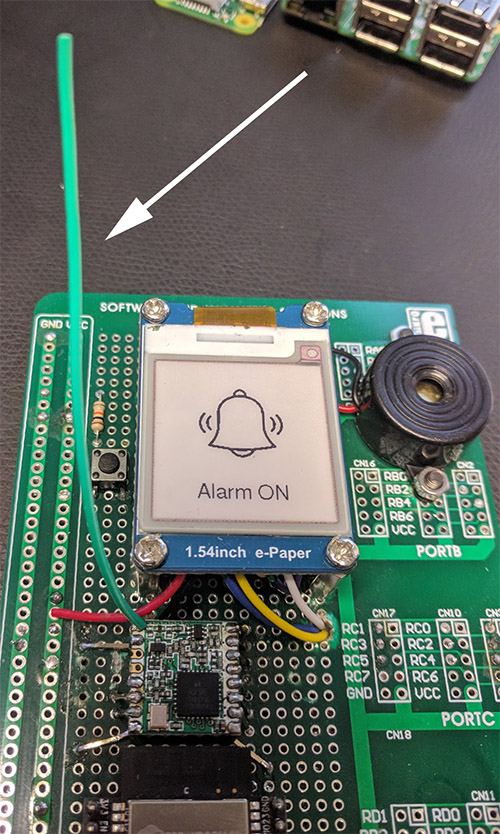
\includegraphics[width=0.675\textwidth]{img/prototype/antenna.jpg}
	\caption[Prototyp 2 Antenne]
	{Prototyp 2 Antenne]}
\end{figure}
\noindent
Die Kommunikation funktioniert einwandfrei und ist mit der des ersten Prototypen vergleichbar. Der Empfang würde mit einer professionellen Antenne noch besser werden. Die Thematik 'Antenne' müsste bei einer Weiterführung des Projektes nochmals beleuchtet werden.
\newpage
\section{Zusammenbau Hardware}
Die Komponenten werden zusammengebaut und untereinander verbunden. Zur besseren Übersicht wird ein Schema  der Elektronik erstellt.
\subsection{Schema}
Die Kommunikation unter den Komponenten wurde im Laufe der Projektarbeit immer unübersichtlicher. Um mir die Arbeit zu erleichtern, wurde ein Schema mit den Komponenten erstellt.\\[0.3cm]
Vor der Arbeit hatte ich noch nie ein Schema gezeichnet und musste mich zuerst einige Stunden in die Materie einarbeiten. Auf anraten einiger Kollegen, mit Erfahrung im Elektronik Umfeld, sowie der frei verfügbaren Lernressourcen und Vorlagen, fiel meine Wahl auf das Programm \textbf{Eagle} der Firma Autodesk \cite{autodesk}. Dank der guten Dokumentation und den Lernvideos auf diversen Plattformen bspw. Youtube kam ich beim Zeichnen schnell vorwärts. \\[0.3cm] 
Ich begann damit Vorlagen der Elektronischen Bausteine/Chips finden. Die Vorlagen zu Lora, GPS, ESP, Schalter und Piezo Lautsprecher konnte ich teilweise vom Hersteller oder von der Community herunterladen und in Eagle importieren. Für das Display musste ich ein bestehende Vorlage eines Displays anpassen. Ich habe dabei die Grösse und die Pinbelegung verändert, damit das Element wie das verwendete Display (Waveshare eInk 200x200) aussieht. \\[0.3cm]
Das Schema ist auf der nachfolgenden Seite abgebildet.
\newpage

\begin{figure}[H]
	\centering
	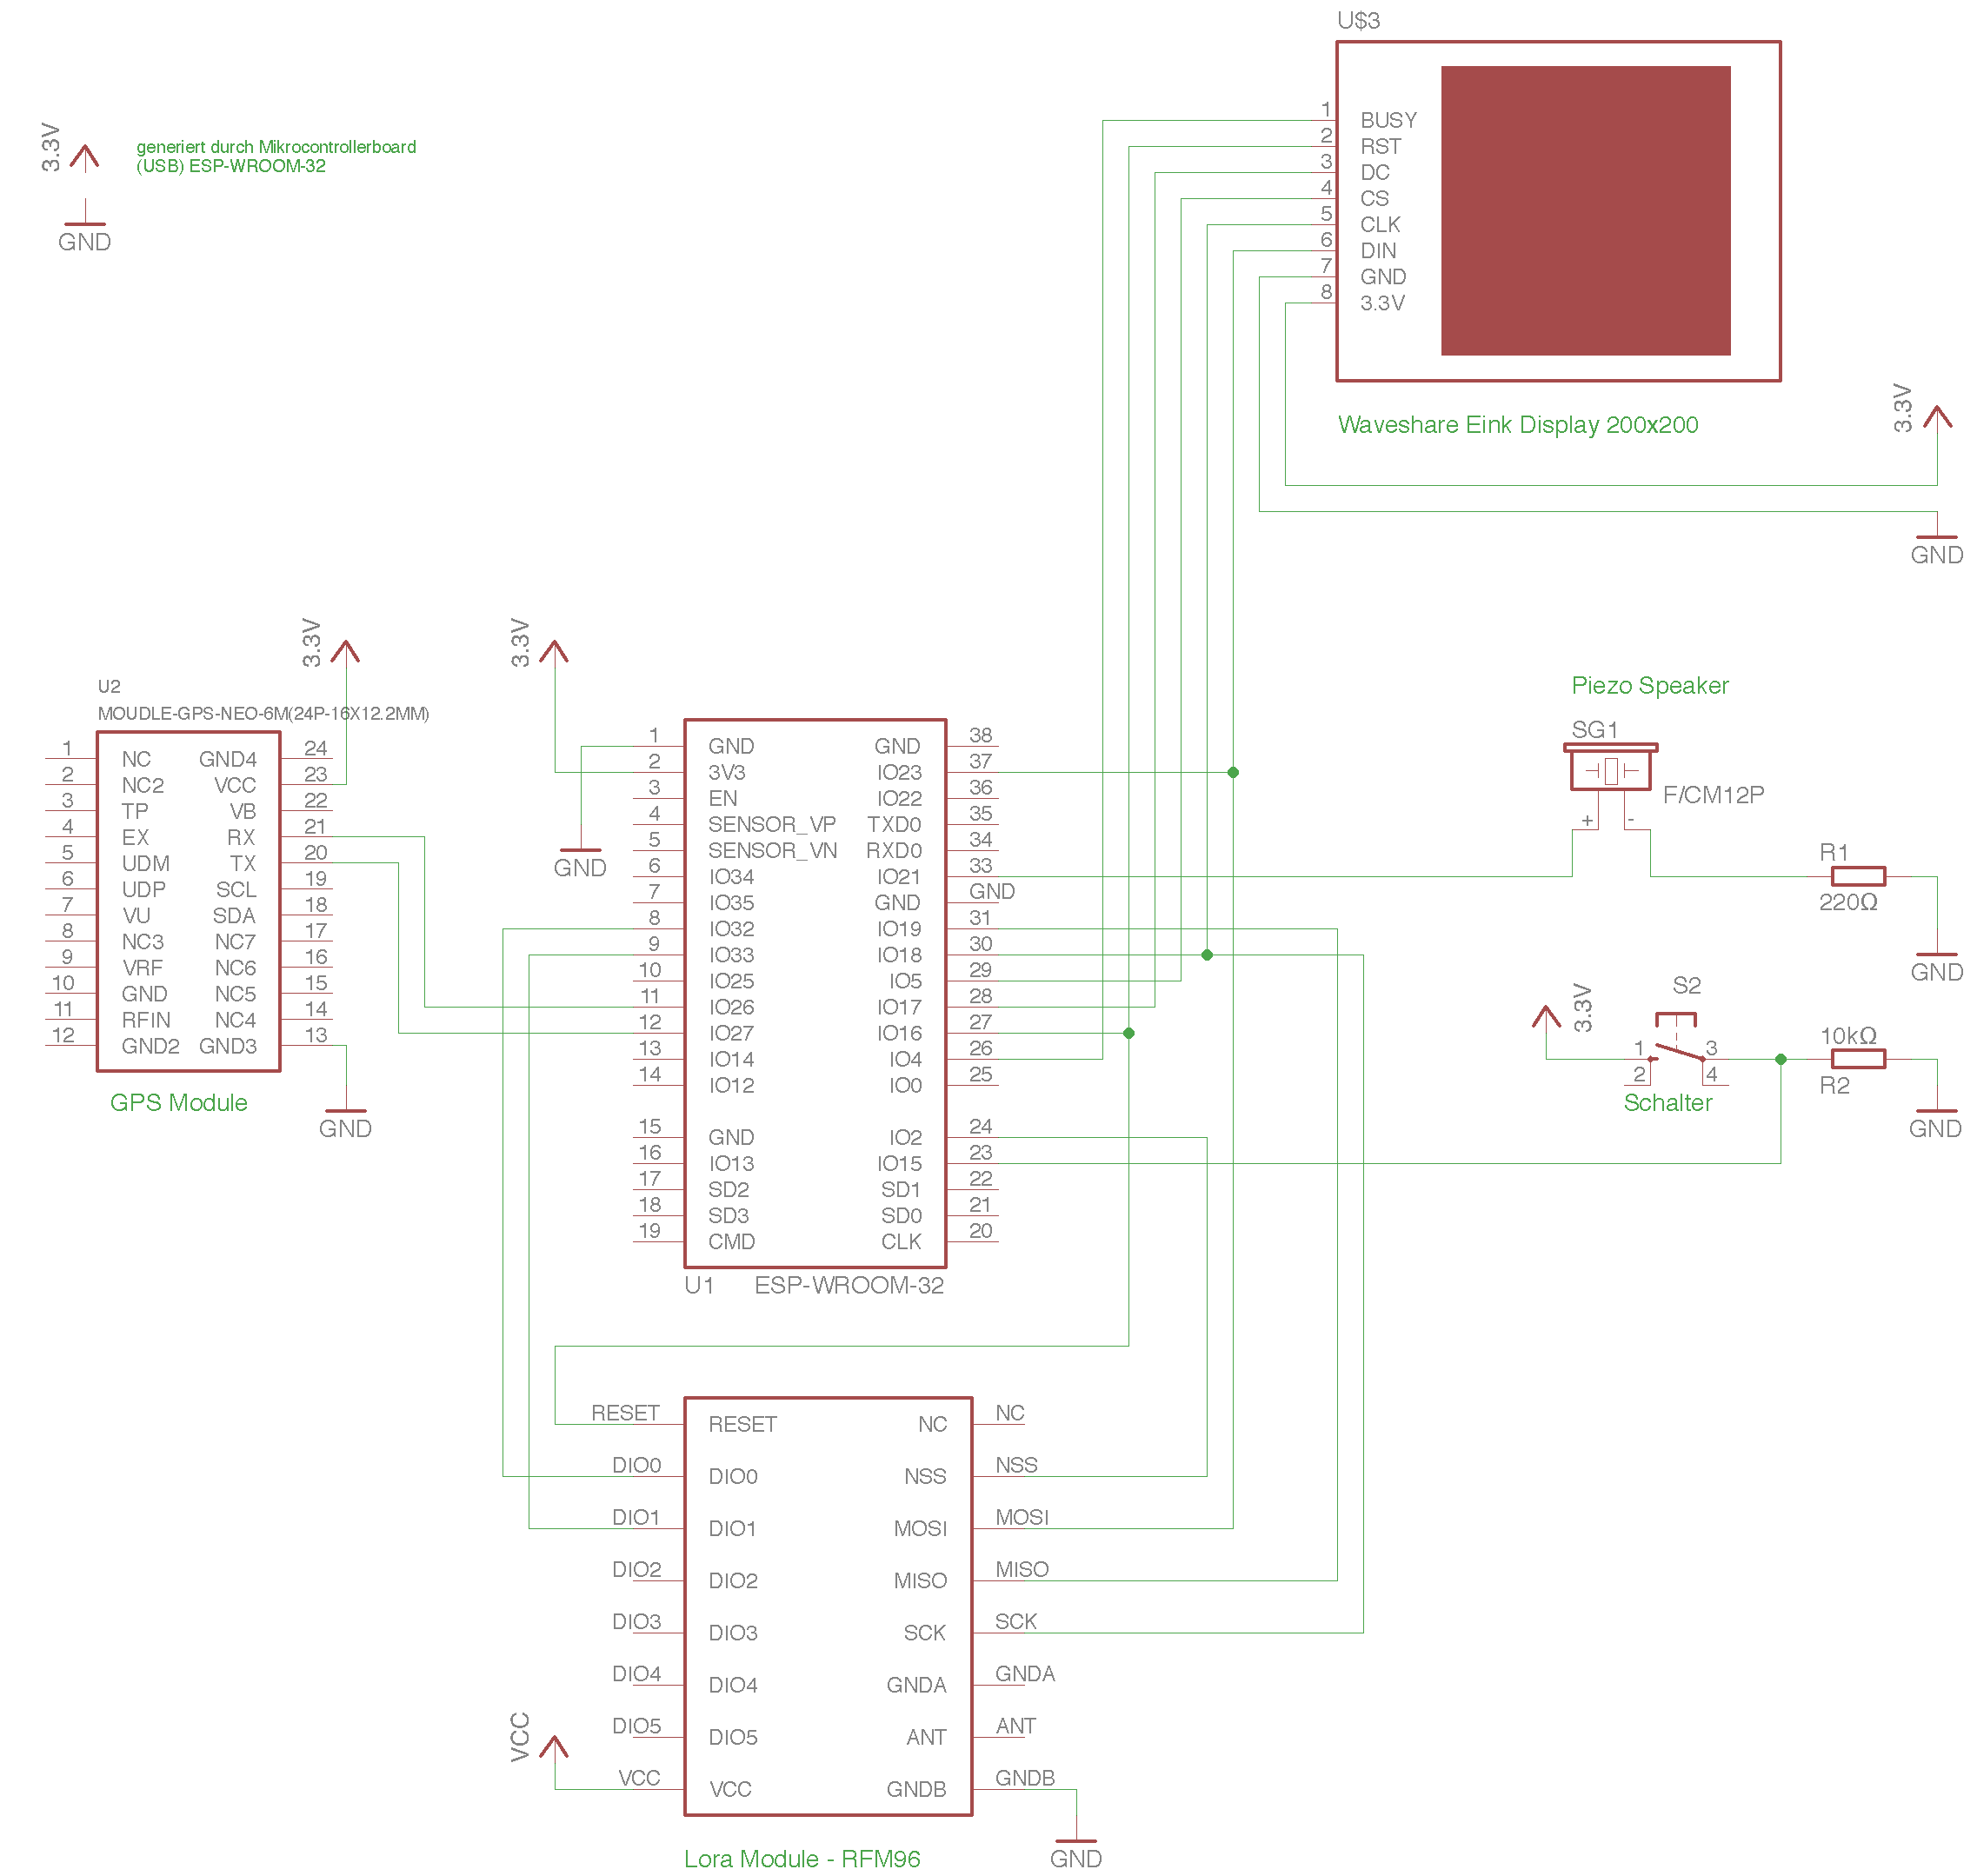
\includegraphics[width=\textwidth]{img/prototype/prototyp_schema.png}
	\caption[Prototyp2 Schema]
	{Prototyp 2 Schema}
\end{figure}

\newpage
\subsection{Mikrocontroller - Pinbelegung}
Die nachfolgende Pinbelegung wurde verwendet um den ESP32 mit den übrigen Komponenten zu verbinden. Zu meiner Überraschung sind die Pins nicht fix durch den ESP32 festgelegt. Die Pins können meist für jegliche Funktion bspw. PWM, SPI verwendet werden. Durch diese Freiheit wird die Verkabelung massiv vereinfacht und die Anzahl der möglichen Fehlerquellen wird reduziert.\\
\begin{tabularx}{\textwidth}{ l|l|X }
	\textbf{MCU Pin} & \textbf{Modul} & \textbf{Funktion}\\ \hline
	IO02 & Lora & SPI ChipSelect (CS)\\\hline
	IO04 & Lora + Display& SPI Busy\\ \hline
	IO05 & Displayl& SPI ChipSelect(CS)\\\hline
	IO15 & Switch & -\\ \hline
	IO16 & Lora + Display & SPI Reset\\\hline
	IO17 & Display&  DataCommand (DC)\\ \hline
	IO18 & Lora + Display & SPI Clock (CLK)\\ \hline
	IO19 & Lora + Display & Master In Slave Out (MISO) \\\hline
	IO21 & Piezo Speaker & - \\ \hline
	IO23 & Lora + Display & SPI Master Out Slave In (MOSI) \\\hline
	IO26 & GPS & UART RX\\ \hline
	IO27 & GPS & UART TX\\ \hline
	IO32 & Lora & DIO0\\ \hline
	IO33 & Lora & DIO1\\ \hline
\end{tabularx}

\newpage
\section{Kommunikation}
In der nachfolgenden Übersicht wird die Kommunikationsart zwischen den Komponenten aufgezeigt.\\
\begin{figure}[H]
	\centering
	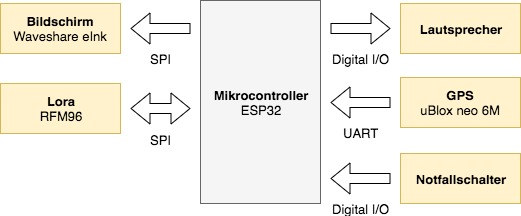
\includegraphics[width=\textwidth]{img/system/ATASNode2_Kommunikation.jpg}
	\caption[Kommunikationsart Prototyp 2]
	{Kommunikationsart Prototyp 2}
\end{figure}

\newpage
\subsection{Zusammenbau}
Die Komponenten wurden auf einer Entwicklungsplatine (PCB Breadboard) platziert und verlötet resp. angeschraubt. Der Mikrocontroller wurde absichtlich nicht im Zentrum platziert, damit der Zugang zum USB Anschluss frei blieb. Abschliessend wurde gemäss Schema die Komponenten untereinander verkabelt.\\
\begin{figure}[H]
	\centering
	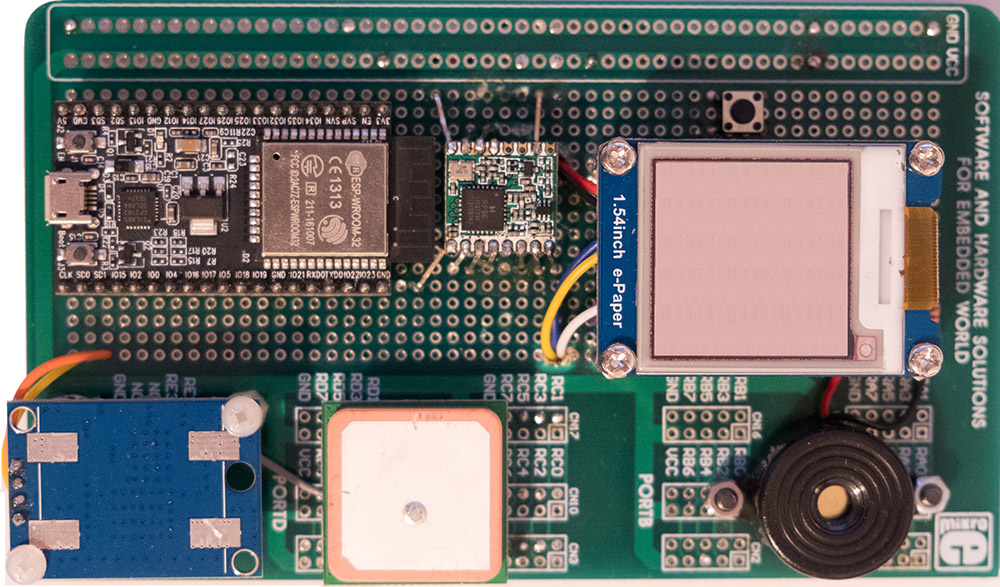
\includegraphics[width=\textwidth]{img/prototype/prototyp2.jpg}
	\caption[Prototyp 2]
	{Prototyp 2}
\end{figure}

\newpage
\section{Software}
Der bestehende Sourcecode des Prototyp 1 kann leider nicht eins zu eins übernommen werden. Die Software ist sehr stark für die Raspberry Pi Umgebung angepasst und ist daher nicht mit dem ESP32 Umfeld kompatibel. Die Software muss portiert werden. Die nachfolgenden Abschnitte beschreiben den Aufbau der Software ATAS-Node welche für den neuen Prototypen angepasst wurde. Die Logik der Software konnte grösstenteils übernommen werden. 

\subsection{Entwicklungsumgebung}
Duch den Umstieg vom Rapberry Pi auf den Mikrocontroller ESP32 hat sich im Bereich der Entwicklungsumgebung einiges verändert. Die ESP32 Plattform unterstützt, Stand heute (16.11.2017), zwei Entwicklungsumgebungen. Das wäre einerseits ESP-IDF (IoT Development Framework) sowie Arduino \cite{espidfarduino}. Die beiden Umgebungen sind miteinander kombinierbar. So kann in der IDF Umfeld die Arduino Unterstützung als Komponente importiert werden. Bestehende für Arduino konzipierte Bibliotheken können dadurch ebenfalls verwendet werden. In Absprache mit dem Betreuer wurde festgelegt, dass die ESP-IDF Umgebung zu verwenden sei. Die Installation der Entwicklungsumgebung ist nicht sonderlich schwer, bedingt aber einige manuelle Schritte. Die Umgebung besteht aus einer Reihe von Tools (Toolchain) zum Kompilieren, Fehlersuche und dem Flashen des Mikrocontrollers.\\[0.3cm]
An dieser Stelle wird auf eine detaillierte Auflistung aller Installationsschritte verzichtet. Die Installation wurde gemäss der Anleitung auf der Webseite der Firma Espressif durchgeführt \cite{espidfinstallation}.\\[0.3cm]
Als Hostsystem wurde ein macOS System verwendet. Damit das System den ESP via USB korrekt erkennen konnte, musste ein zusätzlicher Treiber installiert werden \cite{espidfdriver}. 

\subsection{Sourcecode}
Hinweise wo Sie den Sourcecode einsehen können, finden Sie im Anhang.

\newpage

\subsection{Bibliotheken}
Infolge der Umstellung auf die ESP32 Umgebung mussten einige bestehenden Bibliotheken ersetzte werden. Die verwendeten Software Bibliotheken werden im Anhang aufgeführt.

\subsubsection{LMIC}
Die LMIC Bibliothek hat den LoRaWan Stack implementiert und wird für die korrekte Kommunikation via LoRa Modul benötigt. Zum Zeitpunkt dieser Arbeit gibt es keine für ESP32 portierte LMIC Bibliothek. Für die LoRaWan Kommunikation wurde daher auf eine bestehende Arduino Library (Arduino-LMIC) zurückgegriffen \cite{ArduinoLMIC}. Der Funktionsumfang bleibt der selbe. Den Kommunikationsablauf selbständig zu programmieren hätte den Umfang dieser Arbeit gesprengt. Einige Entwickler berichten von Timing Problemen während der Kommunikation. Bis jetzt konnten beim ATAS Projekt keine Probleme mit der eingesetzten Library festgestellt werden. Die Arduino Library fügt sich problemlos in die ESP-IDF Umgebung ein.

\newpage
\subsection{Klassendiagramm}
Die einzelnen physikalischen Bausteine (GPS, Lora...) werden in Sofware Klassen abgebildet. Die Klassen besitzen entsprechende Methode zum auslesen resp. steuern der Komponenten. Um die Software zu visualisieren wurde ein Klassendiagramm erstellt.
\begin{figure}[H]
	\centering
	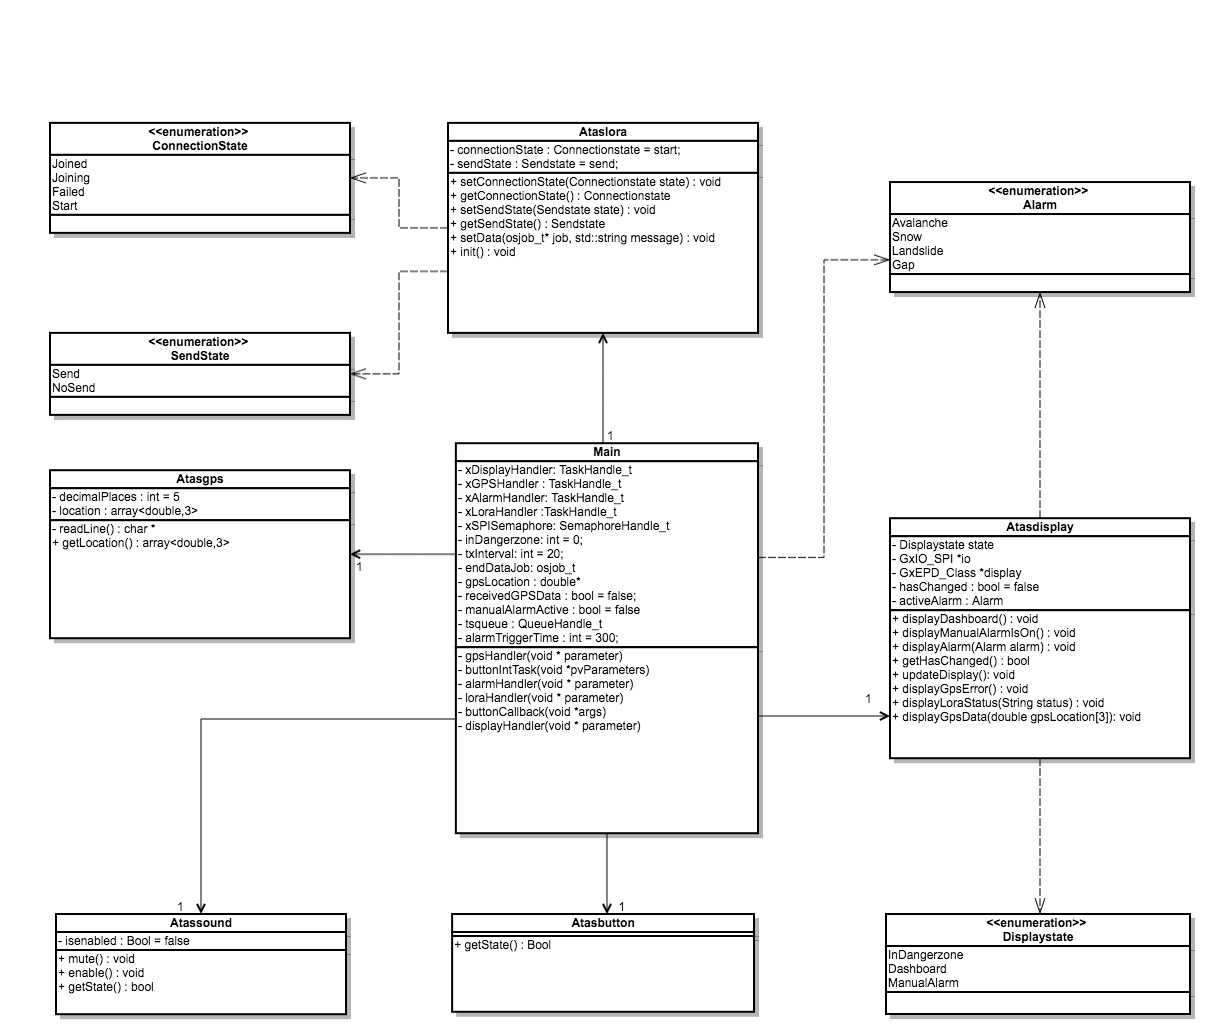
\includegraphics[width=\textwidth]{img/prototype/classdiagram.jpg}
	\caption[Klassendiagramm]
	{Klassendiagramm}
\end{figure}

\newpage
\subsection{Display}
Um die Alarmierung des Alpinisten zu verbessern wurde beim Tracker ein Display eingebaut. Um die Batterie des Trackers nicht weiter zu belasten wurde ein eInk Display ausgewält. Das Display benötigt nur Energie wenn das angezeigte Bild ändert, siehe Abschnitt 'Testing'.\\[0.3cm]
Das Display hat drei Status:
\subsubsection{Dashboard}
Das Dashboard gibt Hinweise zur Lokalisierung (GPS) und der Datenkommunikation (LoRaWan). Das Dashbord ist die Standardansicht, wenn keine Gefahr droht. Im oberen Teil des Bildes werden die GPS Koordinaten und Höhe über Meer angezeigt. Im Unteren Teil finden sich Informationen zur Lora Kommunikation d.H. der Verbindungsstand und der Zeitpunkt der letzten Übertragung (Uplink). Diese Informationen sind für den Alpinisten ein Indikator ob das Gerät einwandfrei funktioniert.\\[0.3cm]
Ein Auszug möglicher Darstellungen auf dem Bildschirm:
\begin{figure}[H]
	\centering
	\begin{subfigure}{.33\textwidth}
		\centering
		\includegraphics[width=0.9\textwidth]{img/prototype/dashboard_idle.jpg}
		\caption[Bildschrim - Start]
		{Startbildschirm}
	\end{subfigure}%
	\begin{subfigure}{.33\textwidth}
		\centering
		\includegraphics[width=0.9\textwidth]{img/prototype/dashboard_joined.jpg}
		\caption[Bildschirm - LoRaWan Verbunden]
		{LoRaWan Verbunden}
	\end{subfigure}%
	\begin{subfigure}{.33\textwidth}
		\centering
		\includegraphics[width=0.9\textwidth]{img/prototype/dashboard_gps.jpg}
		\caption[Bildschirm - GPS Daten]
		{GPS Daten}
	\end{subfigure}%
\end{figure}

\subsubsection{Alarm}
Der Alarm Bildschirm informiert den Alpinisten über mögliche Gefahren.
\begin{figure}[H]
	\centering
	\begin{subfigure}{.25\textwidth}
		\centering
		\includegraphics[width=0.9\textwidth]{img/prototype/avalanche.jpg}
		\caption[Lawine]
		{Lawine}
	\end{subfigure}%
	\begin{subfigure}{.25\textwidth}
		\centering
		\includegraphics[width=0.9\textwidth]{img/prototype/landslide.png}
		\caption[Erdrutch / Steinschlag]
		{Steinschlag}
	\end{subfigure}%
	\begin{subfigure}{.25\textwidth}
		\centering
		\includegraphics[width=0.9\textwidth]{img/prototype/snowflake.jpg}
		\caption[Schneesturm]
		{Schneesturm}
	\end{subfigure}%
	\begin{subfigure}{.25\textwidth}
		\centering
		\includegraphics[width=0.9\textwidth]{img/prototype/crack.jpg}
		\caption[Spalte]
		{Spalte}
	\end{subfigure}%
\end{figure}
\subsubsection{Notfall}
Der Notfall Modus wird vom Alpinisten, durch einen Druck auf den Notfallknopf, selbst ausgelöst. Der Bildschirm dient der Bestätigung für das erfolgreiche aktivieren des Alarms.
\begin{figure}[H]
	\centering
	\includegraphics[width=0.25\textwidth]{img/prototype/alarmbell.jpg}
	\caption[Notfallalarm]
	{Notfallalarm}
\end{figure}%

\newpage
\subsubsection{Herausforderung Timing}
Die Schaltung des Prototypen wurde  so aufgebaut, dass möglichst wenig Kabel gezogen werden mussten. Infolge dessen wurden der Bildschirm  und das LoRa Modul über einen einzigen SPI Kontroller angesteuert. Relativ schnell machte sich ein Timing Problem bemerkbar. Die Software versuchte das Display zu aktualisieren und im gleichen Moment Daten per LoRa versenden. Die Kommunikation mit dem Bildschirm wurde gestört, der Bildaufbau wurde unterbrochen
\begin{figure}[H]
	\centering
	\includegraphics[width=0.4\textwidth]{img/prototype/display_updateissue.jpg}
	\caption[Fehlerhafter Bildaufbau Display]
	{Fehlerhafter Bildaufbau Display}
\end{figure}
\noindent
Um die korrekte Datenübertragung sicherzustellen, wurde in der Software ein Mutex implementiert. Die Ansteuerung des Bildschirm und des LoRa Kommunikation wurde in zwei unabhängige Tasks aufgeteilt. Ist ein Task beschäftigt Daten zu senden, wird die Mutex Ressource gesperrt. Der andere Tasks muss warten, bis er wieder Daten senden kann. Mit dieser Lösung kann sichergestellt werden, dass es zukünftig keine Kommunikationskonflikte mehr geben wird.
\begin{figure}[H]
	\centering
	\begin{subfigure}{.5\textwidth}
		\centering
		\includegraphics[width=0.9\textwidth]{img/prototype/displaymutex.png}
		\caption[Mutex - Bildschrim]
		{Mutex - Bildschirm}
	\end{subfigure}%
	\begin{subfigure}{.5\textwidth}
		\centering
		\includegraphics[width=0.9\textwidth]{img/prototype/loramutex.png}
		\caption[Mutex - Lora]
		{Mutex - Lora}
	\end{subfigure}%
\end{figure}
\newpage

\newpage
\section{Prototyp Testing}
Abschliessend werden Tests mit dem neuen Tracker durchgeführt.

\subsection{Energieversorgung}
Einer der Hauptgründe für den Bau eines neuen Prototypen, ist der Energieverbrauch. In einem abschliessenden Test soll nun festgestellt werden, wie sich der Energiebedarf des ersten zum zweiten Prototypen verändert hat. Folgende Szenarien resp. Systemzustände sollen geprüft werden:
\begin{itemize}
	\item Ruhezustand
	\item Daten senden via LoRa
	\item Bildschirm aktualisieren
	\item Lautsprecher ein	
\end{itemize}
\textbf{Ausgangslage}: Das Gerät wird an ein Speisegerät angeschlossen. Die Betriebsspannung beträgt bei beiden Geräten 5V. Die beiden Prototypen verfügen über einen eingebauten Spannungswandler welche die Spannung auf 3.3V herunter regelt. Die dabei entstehenden Verlustleistung wird bei den nachfolgenden Tests ignoriert. Während des Tests sind alle Module (LoRa, GPS... ) angeschlossen, werden also mit Strom versorgt. Der Prototyp 1 verfügt über kein Display, deshalb können keine Daten für diesen Systemzustand erhoben werden. Die entsprechenden Szenarien werden beim Prototypen einstellt und die benötige Leistung werden vom Speisegerät abgelesen.

\newpage
\noindent
\textbf{Messresultate:}
\begin{figure}[H]
	\centering
	\includegraphics[width=\textwidth]{img/testing/energy_usage.jpg}
	\caption[Gesamt Energieverbrauch pro Prototyp]
	{Gesamt Energieverbrauch pro Prototyp}
\end{figure}
\noindent
Diese Grafik zeigt den gesamten Energieverbrauch des Systems während der durchgeführten Aktion.
Wie in der Grafik ersichtlich, benötigt der Prototyp 1 im Ruhezustand (0.4W) ca. 4 mal soviel Energie wie der neue Prototypen (1.6W). Durch den Wechsel der Hardware konnte der Energieverbrauch drastisch gesenkt werden.\\[0.3cm]
Das senden der Daten lässt den Energieverbrauch stark ansteigen. Beim Prototypen 2 wächst der Verbrauch gar um 100\%. Das senden via LoRa macht also einen grossen Teil des Energieverbrauchs aus.
\newpage
\begin{figure}[H]
\centering
\includegraphics[width=\textwidth]{img/testing/energy_usage_perAction.jpg}
\caption[Veränderung des Energieverbrauchs zum Ruhezustand]
{Veränderung des Energieverbrauchs zum Ruhezustand}
\end{figure}
\noindent
Der Gesamtverbrauch des Systems während einer Aktion wurde mit dem Verbrauch des Ruhezustandes subtrahiert. Diese Grafik zeigt nun wie die einzelnen Aktionen den Energieverbrauch beeinflussen. Die nachfolgenden Erkenntnisse wurden daraus gewonnen
\begin{itemize}
\item Da auf beiden Prototypen der gleiche LoRa Chip verbaut ist, ist es keine Überraschung, dass die benötigte Energie in etwa identisch ist. 
\item Das Aktualisieren des Displays benötigt, im Vergleich zum Senden via LoRa,  sehr wenig Energie.
\item Das Aktivieren des Piezo Lautsprechers hat keinen messbaren Einfluss auf den Energieverbrauch.
\end{itemize}

\newpage
\subsection{Schlusswort}
Die Resultate mit dem neuen Prototypen sind zufriedenstellend. Das Display erweitert den Prototypen um ein wichtiges Mittel der Alarmierung. Das System konnte in Sachen Energiebedarf optimiert werden. Der Prototyp 2 funktioniert einwandfrei. Dem nächsten Schritt, dem finalen Prototypen steht somit nichts mehr im Weg.


% ***** TESTING *****
\chapter{Testing Datenübertragung }
Ein Teil des Systemaufbaus aus dem vorgängigen Projekt soll getestet werden. In diesem Kapitel wird genau beschrieben, wie beim Testing des Systems vorgegangen wird.
\section{Ablauf Vorgehen}
In der nächsten Abbildung sind die geplanten Schritte aufgeführt.
\begin{figure}[h]
	\centering
	\includegraphics[width=\textwidth]{img/projectFlow_testing.png}
	\caption[Flowchart Testing]
	{Ablauf Testing}
\end{figure}
\\ 
Die einzelnen Schritte werden auf den kommenden Seiten detailliert erklärt.
\newpage
\section{Definition}
Es muss definiert werden
\begin{itemize}
	\item Welche Komponenten geprüft werden sollen.\\[0.3cm]
	Während der Arbeit soll die Kommunikation zwischen dem Tracker (ATAS-Node) und dem Gateway getestet werden.
	\item Welche Aspekte der Komponente sollen betrachtet werden.\\[0.3cm]
	Der Fokus liegt auf der \textbf{Zuverlässigkeit} der Übertragung. Mich interessiert, wie sicher es ist, dass eine Meldung ihr Ziel erreicht. 
	\item Mit welchen Mitteln resp. Messinstrumenten gemessen wird.\\[0.3cm]	
	Das TTN Netzwerk bietet uns die Möglichkeit mittels Dashboard einzusehen, wann welche Pakete auf dem Gateway eintreffen.So können wir prüfen ob die Verbindung zwischen Gateway und Tracker funktioniert. \\
	
	\begin{minipage}{\linewidth}
		\centering
		\includegraphics[width=\linewidth]{img/ttn/ttn_messages}
		\captionof{figure}{TTN Messages}
	\end{minipage}

	Diese Ansicht gibt uns einen guten Überblick. Leider müssen die Daten alle manuell herauskopiert werden um diese analysieren zu können. Es gibt momentan keine Möglichkeit die gesamten Daten von TTN herunterzuladen. Diese Tatsache macht die Auswertung der Daten bspw. mit Excel sehr umständlich.
	
	\item Welche Daten können untersucht werden.\\[0.3cm]
	Für die Messungen sind mehre Daten von Interesse. Dazu gehören: 
	\begin{itemize}
		\item Signalstärke
		\item Wie viele Pakete gehen verloren
		\item Distanz der Übertragung
		\item Sichtverhältnisse zwischen Sender und Empfänger
	\end{itemize}
\end{itemize}

\subsection{Schlussfolgerung}
Wir fassen zusammen:
\begin{itemize}
	\item
	Es muss eine Testumgebung aufgebaut und die Verbindung getestet werden. Um von den bestehenden TTN Gateways unabhängig zu sein, wird ein \textbf{eigener Gateway} aufgebaut.
	\item 
	Da das TTN Dashboard uns keine vernünftige Lösung bietet die Daten auszuwerten, soll eine eigene Lösung entwickelt werden. Die Komponenten ATAS-Web und ATAS-Service müssen entsprechend erweitert werden.
	\item Abschliessend werden mehrere Tests durchgeführt. Die Verbindung wird aufgebaut und mittels neu entwickeltem Dashboard geprüft.
\end{itemize}

\newpage
\section{Standort}
Ausgehend von den vorangegangen Definitionen muss folgendes definiert werden.
\begin{itemize}
	\item Es muss ein Ort gefunden werden, wo der Gateway platziert werden kann.\\[0.3cm]
	Der Standort kann frei gewählt werden. Zwei Kriterien müssen zwingend erfüllt sein. 
	\begin{enumerate}
		\item
		Der Gateway empfängt die Daten der Endgeräte und muss diese dem TTN Netzwerk über das Internet weiterleiten können. Eine stabile Internetverbindung ist nötig. 
		\item 
		Der Standort sollte in der nähe von möglichen Wanderrouten resp. Testbereichen liegen.
	\end{enumerate}
	\item Für die Tests sollten mind. 2 Routen/Wanderungen definiert werden. Dies garantiert eine vernünftige Anzahl an Messwerten.
	\item Auf dem Pfad selbst werden Orte definiert wo die Verbindungstests durchgeführt werden.
\end{itemize}

\newpage
\subsection{Gateway}
Der Standort für den LoRa Gateway war schnell gefunden. Ich arbeite momentan als Informatik Systemengineer bei der Hoffmann Neopad AG. Die Firma besitzt eine Niederlassung in der Nähe der Stadt Thun (BE). Das Gebäude ist 2 Stockwerke hoch und die Adresse liegt in unmittelbarer nähe der Voralpen. Hohe Berge für einen möglichen Testlauf sind max. 20km entfernt. Dazu zählen beispielsweise das Stockhorn, Niesen sowie das Niederhorn.\\[0.1cm]
\begin{tabularx}{\textwidth}{ l|X }
		\textbf{Beschreibung} & \textbf{Bild} \\ \hline
		Standort Hoffmann Neopac AG & \parbox[c]{1em}{
			\vspace{8pt}\includegraphics[width=0.6\textwidth]{img/gateway/gateway_map.jpg}\vspace{8pt}} \\ \hline
		Standort Gateway auf Gebäude &  \parbox[c]{1em}{
			\vspace{8pt}\includegraphics[width=0.6\textwidth]{img/gateway/gateway_building_front.jpg}\vspace{8pt}} \\ \hline
\end{tabularx}

\newpage
\subsection{Testregionen}
Im ersten Teil meiner Arbeit konzentrierte ich mich stark auf den Aufbau des Prototypen. Für die Testphase wurde im Projekt zu wenig Zeit eingeplant, was sich im Verlauf des Projekts als Problematisch herausgestellt hat. Der Winter liess, wie sonst nicht üblich, nicht lange auf sich warten. Bereits Mitte Oktober beginn es zu schneien. Wanderrouten/ Regionen welche ich für das Testing verwenden wollte, bspw. der Nordaufstieg Stockhorn, wurden wegen zu hoher Lawinengefahr geschlossen.\\[0.3cm]
Nichtsdestotrotz konnte ich 2 Testregionen definieren, welche einfach zugänglich und soweit gefahrlos passierbar waren.
\begin{tabularx}{\textwidth}{ l|X }
	\textbf{Region 1: Niederhorn} & \textbf{Bild} \\ \hline
	Region &  \parbox[c]{1em}{
		\vspace{8pt}\includegraphics[width=0.6\textwidth]{img/testregions/niederhorn.png}\vspace{8pt}} \\ \hline
	Höhenunterschied zum Gateway&\parbox[c]{1em}{
		\vspace{8pt}\includegraphics[width=0.6\textwidth]{img/testregions/niederhorn_altitude.png}\vspace{8pt}} \\ \hline
	Mittlere Distanz zum Gateway & 15Km \\ \hline
\end{tabularx}

\newpage
\begin{tabularx}{\textwidth}{ l|X }
	\textbf{Region 2: Heiligenschwendi} & \textbf{Bild} \\ \hline
	Region & \parbox[c]{1em}{
		\vspace{8pt}\includegraphics[width=0.6\textwidth]{img/testregions/heiligenschwendi.png}\vspace{8pt}} \\ \hline
	Höhenunterschied zum Gateway&\parbox[c]{1em}{
		\vspace{8pt}\includegraphics[width=0.6\textwidth]{img/testregions/heiligenschwendi_altitude.png}\vspace{8pt}} \\ \hline
	Mittlere Distanz zum Gateway & 7Km \\ \hline
\end{tabularx}

\newpage
\section{Aufbau \& Vorbereitungen}
\subsection{Gateway}
In diesem Abschnitt ist der Aufbau des LoRaWan Gateways beschrieben. Der Gateway besteht aus den folgenden Komponenten
\begin{itemize}
	\item A: Raspberry Pi 3
	\item B: IMST iC880a Board \cite{ic880}
	\item C: IP67-Box
\end{itemize}
\begin{figure}[h]
	\centering
	\includegraphics[width=\textwidth]{img/gateway/gateway.jpg}\\[0.3cm]
	\caption[Gateway]
	{Gateway}
\end{figure}
Durch den Einsatz einer IP67 Box sind die elektronischen Komponenten gegen Staub und Wasser geschützt.

\newpage
\subsubsection{Installation}
Die Webressourcen der TTN Community von Zürich waren bei der Installation eine grosse Hilfe \cite{ttnzürich}. Das Raspberry PI und das iC880 Board wurden gemäss der Webseite verkabelt.\\[0.3cm]
Die Community hat ein sehr simples Installationsskript zusammengestellt um die Gateway Software automatisiert zu installieren. Folgende Schritte wurden auf dem Raspberr PI durchgeführt.
\lstset{language=C++}
\begin{lstlisting}
// update software
sudo apt-get update
sudo apt-get upgrade
sudo apt-get install git

// set local & timezone
sudo dpkg-reconfigure locales // de_CH
sudo dpkg-reconfigure tzdata // Europe/Zurich

// Enable SPI, Interfacing options -> P4 SPI
sudo raspi-config

// Reboot
reboot

// Install Gateway Software
git clone https://github.com/ttn-zh/ic880a-gateway.git ~/ic880a-gateway
cd ~/ic880a-gateway
sudo ./install.sh spi
\end{lstlisting}
Alles in allem eine sehr einfache Prozedur die nicht viel zeit in Anspruch genommen hat. Anhand der Mac Adresse des Raspberry PI wird im Abschluss des Skripts eine EUI generiert.
\newpage
\subsubsection{TTN Registrierung}
Mit der vorher generierten EUI kann der Gateway nun auf dem TTN Dashboard registriert werden.
\begin{figure}[H]
	\centering
	\includegraphics[width=0.9\textwidth]{img/gateway/ttn_gateway.png}
	\caption[TTN Dashboard Gateway]
	{TTN Dashboard Gateway}
\end{figure}
\noindent
Der Gateway ist nun online und leitet Datenpakete weiter.
\begin{figure}[H]
	\centering
	\includegraphics[width=0.9\textwidth]{img/gateway/ttn_gateway_done.png}
	\caption[TTN Dashboard Gateway Registriert]
	{TTN Dashboard Gateway Registriert}
\end{figure}

\newpage
\subsection{Dashboard}
Das eingeschränkte TTN Dashboard genügt für das Testing nicht. In diesem Abschnitt wird erklärt, wie die ATAS Software erweitert wurde, um die Testdaten besser analysieren zu können.
\subsubsection{ATAS-Web}
Die Webkomponente ATAS-Web wurde um einige Funktionen erweitert. Über den Menüpunkt \textbf{'Data'} kann das Dashboard aufgerufen werden.
\begin{figure}[H]
	\centering
	\includegraphics[width=\textwidth]{img/testing/atasweb_menu.jpg}
	\caption[ATAS-Web Menu]
	{ATAS-Web Menu}
\end{figure}

\newpage
\noindent
Das Dashboard bietet folgende Funktionen.
\begin{itemize}
	\item A: Über ein Dropdown kann der entsprechende Tracker ausgewählt werden.
	\item B: Da eine Uplink Nachricht von mehreren Gateways empfangen werden kann, ist es nötig die Nachrichten nach Gateway zu filtern.
	\item C: Die aktuell angezeigten Daten können als CSV Datei heruntergeladen werden.
	\item D: das Dashboard zeigt die empfangenen Uplink Nachrichten an. 
\end{itemize}
\begin{figure}[H]
	\centering
	\includegraphics[width=\textwidth]{img/testing/atasweb_data.jpg}
	\caption[ATAS-Web Dashboard]
	{ATAS-Web Dashboard}
\end{figure}

\newpage
\section{Messungen}
Es werden verschiedene Testszenarien definiert.

\subsection{Test 1: Praxistest}
\subsubsection{Vorgehen}
Das ATAS System soll geprüft werden ob es praxistauglich ist. Um dies zu überprüfen, wird in der vorher definierten Testregion 2, Messungen durchgeführt. Es soll getestet werden, wie zuverlässig die Übertragung funktioniert.\\[0.3cm]
Für diesen Test werden die folgenden Daten erhoben:
\begin{enumerate}
	\item Distanz zwischen Sender und Empfänger
	\item Signal to Noise Ratio (SNR)
	\item RSSI
	\item Sichtverhältnisse zwischen Sender und Empfänger
\end{enumerate}	
Die erhobenen Daten werden nach Sichtverhältnissen kategorisiert. Messungen sollen in 3 Kategorien eingeteilt werden.
\begin{enumerate}
	\item A: Direkter Sichtkontakt
	\item B: Wenig Sichtkontakt resp. teilweise blockiert. Bspw. durch Bewaldung oder Steinformationen
	\item C: kein ein Sichtkontakt zwischen Empfänger und Sender.
\end{enumerate}
\subsubsection{Ausgangslage}
Die Tests werden mit einem fixen Einstellungen durchgeführt:
\begin{enumerate}
	\item Spreadingfactor SF12
	\item Bandbreite 125KHz
	\item Coding Rate 4/8
\end{enumerate}
Zum Zeitpunkt des Tests (13.12.2017) lag über 20cm Schnee.
\newpage
\subsubsection{Resultate}
\begin{figure}[H]
	\centering
	\includegraphics[width=\textwidth]{img/testing/testing3_lostpackets.png}
	\caption[Test 1 Resultate]
	{Test 1 Resultate}
\end{figure}

\newpage
\subsubsection{Auswertung}
Die Resultate des ersten Tests decken etwas sehr interessantes auf. Die Distanz zwischen Gateway und Tracker hat einen sehr kleinen Einfluss auf die Übertragungsqualität. Wie wir vom letzten Datenpunkt ablesen können, ist es auch mit einer Distanz von über 7Km möglich, ein Signal sauber zu übertragen. Mehr Einfluss haben die Hindernisse zwischen Sender und Empfänger. Ist ein Hindernis bspw. ein Hügel im Weg, wird die Übertragung massiv gestört.\\[0.3cm]
Beim Datenpunkt 7 konnten keine Pakete empfangen werden. Die Messung wurde auf der Gateway abgewendeten Talseite durchgeführt. Solche grossen Hindernisse vermag das Signal also nicht zu durchdringen.

\begin{figure}[H]
	\centering
	\includegraphics[width=\textwidth]{img/testing/testing3_graphic.jpg}
	\caption[Darstellung: Messung 7]
	{Darstellung: Messung 7}
\end{figure}

\newpage
\subsection{Test 2: Spreadingfactor}
Es soll geprüft werden, wie sich der LoRa Spreadingfactor auf die Übertragung von Daten auswirkt.
Für diesen Test werden die folgenden Daten erhoben:
\begin{enumerate}
	\item Spreading Factor
	\item Signal to Noise Ratio
	\item RSSI
\end{enumerate}
\subsubsection{Test 2.1}
\textbf{Ausgangslage:} Die Messungen werden in der Region 1 durchgeführt. Der Standort wird nicht gewechselt. Die Distanz zwischen Gateway und Tracker bleiben also gleich. Es werden pro Spreading Factor (7-12), 10 Messungen durchgeführt. Der kleinste wie auch der grösste Messwert werden entfernt. Damit soll verhindert werden, dass Ausreisser die Statistik stören. Damit bleiben uns 8 Messpunkte. \\[0.3cm]
\textbf{Annahme:} Gemäss Literatur müsste klar erkennbar werden, dass bei einem höheren SF Wert, das Signal mit weniger Störung übertragen werden kann, dH. Das Signal stärker beim Gateway eintrifft.\\[0.3cm]
\textbf{Die Messresultate:}
\begin{figure}[H]
	\centering
		\includegraphics[width=\textwidth]{img/testing/testing1_sf_snr.jpg}
		\caption[Messwerte SNR  pro Spreadingfactor]
		{Messwerte SNR pro Spreadingfactor}
\end{figure}
\begin{figure}[H]
	\centering
	\includegraphics[width=\textwidth]{img/testing/testing1_sf_rssi.jpg}
	\caption[Messwerte RSSI pro Spreadingfactor]
	{Messwerte RSSI pro Spreadingfactor}
\end{figure}
\noindent
Wie bei den Resultaten ersichtlich, ist die Annahme nicht eingetroffen. Es ist kein Muster erkennbar, das bei einem höheren SF ein besseres Signal zu erwarten ist. Ich gehe davon aus, dass für einen solchen Test mehr Messwerte von Nöten sind. Ich werde den Test also mit mehr Messwerten wiederholen müssen. Für SF7 konnten keine Pakete zugestellt werden. Entweder hatte der Gateway eine Fehlfunktion, oder die Distanz war zu Gross als dass dieser die Daten hätte empfangen können.
\newpage
\subsubsection{Test 2.2}
\textbf{Ausgangslage:} Analog Test 2.1. Die Messungen werden in der Region 2 durchgeführt. Anstatt wie im ersten Test 10 Messungen durchzuführen, wird die Anzahl auf 50 erhöht. Ausreisser werden ebenfalls wieder entfernt. 20\% der Messwerte fallen weg. Damit bleiben 40 Messpunkte.\\[0.3cm]
\textbf{Annahme:} Ananlog Test 2.1\\[0.3cm]
\textbf{Die Messresultate:}
\begin{figure}[H]
	\centering
	\includegraphics[width=\textwidth]{img/testing/testing2_sf_snr.jpg}
	\caption[Messwerte SNR  pro Spreadingfactor]
	{Messwerte SNR pro Spreadingfactor}
\end{figure}
\begin{figure}[H]
	\centering
	\includegraphics[width=\textwidth]{img/testing/testing2_sf_rssi.jpg}
	\caption[Messwerte RSSI pro Spreadingfactor]
	{Messwerte RSSI pro Spreadingfactor}
\end{figure}
\noindent
Auch mit mehr Messwerten ist die Annahme nicht eingetroffen. Warum sich die Messwerte von der Literatur distanzieren ist zum jetzigen Zeitpunkt nicht bekannt.

\newpage
\subsection{Test 3: Datenrate}
\textbf{Ausgangslage:} In diesem Test soll ermittelt werden, wie häufig wir die Daten des Trackers übermitteln können. Die maximal zu übertragende Datengrösse wurde bereits in einem vorhergehenden Abschnitt definiert und beträgt \textbf{20Bytes}. Die Coding Rate wird auf 4/8 gesetzt.\\[0.3cm]
\textbf{Vorgehen:} Pro Spreadingfactor werden Messungen durchgeführt. Die Zeitdifferenz zwischen den Übertragungen wird ermittelt.\\[0.3cm]
\textbf{Messresultate:} 
\begin{figure}[H]
	\centering
	\includegraphics[width=\textwidth]{img/testing/timebetweenpakets.jpg}
	\caption[Zeit zwischen zwei Paketen]
	{Zeit zwischen zwei Paketen}
\end{figure}
\noindent
Auch bei SF12 liegt die Zeit zwischen den Übertragungen bei nur 170 Sekunden. Das bedeutet, dass wir ca. alle 3 Minuten den neue Standort übermitteln können. Beim Wandern wir diese Rate ausreichen. Ob diese Zeit für Skifahrer reicht müssten in weiteren Tests festgestellt werden. Würden wir, wie bereits angesprochen, eine eigen ADR Lösung implementieren könnten wir den SF auch reduzieren. Dies würde und ermöglichen schneller zu übertragen.

\newpage
\subsection{Ergebnisse}
Aus den gewonnen Resultaten lässt sich bereits ableiten, ob das ATAS System praxistauglich ist. Beim ersten Tests haben wir festgestellt, dass sobald sich ein Hindernis bspw. ein Hügel oder viele Bäume zwischen Tracker und Gateway befindet, die Übertragung sehr stark gestört wird. Befinden wir uns auf der Gateway abgewendeten Talseite, kann teilweise kein Signal mehr zum Gateway durchdringen. Würden wir nun auf der anderen Seite des Berges einen weiteren Gateway installieren wäre das Problem gelöst, die Übertragung würde wieder funktionieren. Die Form erinnert zwar von der Seite betrachtet meist an ein Dreieck, in der Realität sieht es aber oft anders aus. Die Berge sind aber eine sehr dynamische Landschaft. Ein bildliches Beispiel:
\begin{figure}[H]
	\centering
	\includegraphics[width=\textwidth]{img/testing/testing_result.png}
	\caption[Dynamische Berglandschaft Beispiel]
	{Dynamische Berglandschaft Beispiel}
\end{figure}
\noindent
Befindet sich der Alpinist an einer solchen Position werden viele Übertragungen fehlschlagen. Die Ortung funktioniert nicht mehr korrekt und die Sicherheit der Person kann nicht mehr gewährleistet werden. \\[0.3cm]
\textbf{Damit kommen wir zum Schluss, dass das ATAS System, mit LoRa als Kommunikationslösung, nicht praxistauglich ist.}

\chapter{Schlusswort}
\section{Verbesserungsvorschläge}
\subsection{Automatischer Datenaustausch}
Zurzeit werden die Gefahrenzonen manuell über eine Webapplikation (ATAS-Web) erfasst. Die Daten können täglich ändern. Eine manuelle Bearbeitung ist daher weder effizient noch alltagstauglich. Sollte das Projekt in irgend einer Form weitergeführt werden, müssten Lieferanten für solche Gefahrenzoneninformationen gefunden werden. Die  Provider müssen Schnittstellen anbieten bspw. REST oder MQTT damit wir die Daten automatisiert in den ATAS-Service importieren können. 

\begin{figure}[H]
	\centering
	\includegraphics[width=0.6\textwidth]{img/system/ATAS_ExternalAccess.jpg}
	\caption[Gefahrenzonen Provider]
	{Gefahrenzonen Provider}
\end{figure}

\subsection{Wireless Kommunikation}
Die gefundenen Resultate sind auf den ersten Blick vielversprechend. LoRa bringt die benötigte Reichweite, ist stromsparend und die Datenrate würde für dieses Projekt ausreichen. Die Tatsache, dass gewisse Positionen vom Signal her nicht abgedeckt werden können ist aber aus meiner Sicht ein klares Zeichen, dass sich die Technologie nicht eignet. Die Berge und deren Strukturen sind unberechenbar.
\\[0.3cm]
In meinen Augen muss man sich von LoRa und LoRa Wan als Kommunikationsart verabschieden und auf andere Technologien setzen. Sobald Sigfox in der Schweiz verfügbar ist, wäre es sehr interessant auch mit dieser Technologie entsprechende Tests durchzuführen. Ich befürchte aber, das eine Übertragungsart, bei welcher der Gateway in einem Tal positioniert ist, nie 100\% funktionieren wird. Als Alternative sehe ich hier Satellitentechnologien.Der Raum gegen Oben, sprich zum Satellit, ist im Normalfall aber frei. Eine Übertragung sollte immer und überall funktionieren. Diese Form der Kommunikation wirft dann natürlich neue Fragen auf. Wie hoch sind die Kosten für die Nutzung eines solches Services? Wie lange hält die Batterie über diese Kommunikationsart?

\section{Rückblick Projekt}
Rückblickend kann ich sagen, dass es im Verlauf des Projekts bezüglich des Aufwands, zu Fehleinschätzungen gekommen ist. Eine Wanderung, mit Messungen, Anfahrt und anschliessender Auswertung der Daten hat viel mehr Zeit in Anspruch genommen als im Projekt eingeplant war.\\[0.3cm]
Nichtsdestotrotz schaue ich auf ein erfolgreiches Projekt zurück. Ich konnte an die Arbeit aus dem Vorprojekt 'Projekt 2' gut anknüpfen. Während der Bachelorarbeit war es mir möglich, mich intensiver mit den Technologien und damit verbundenen Fragestellungen zu befassen. Die Ergebnisse der Arbeit sind sehr interessant und zeigen auf wo die Grenzen der heutigen Technik liegen. Ich bin überzeugt, dass ATAS mit der richtigen Kommunikationstechnologie ein vielversprechendes Projekt darstellt.

\chapter*{Selbständigkeitserklärung}
\label{chap:selbstaendigkeitserklaerung}

\vspace*{10mm} 

Ich bestätige, dass ich die vorliegende Arbeit selbstständig und ohne Benutzung anderer als der im Literaturverzeichnis angegebenen Quellen und Hilfsmittel angefertigt habe. Sämtliche Textstellen, die nicht von mir stammen, sind als Zitate gekennzeichnet und mit dem genauen Hinweis auf ihre Herkunft versehen. 

\vspace{15mm}

\begin{tabbing}
xxxxxxxxxxxxxxxxxxxxxxxxx\=xxxxxxxxxxxxxxxxxxxxxxxxxxxxxx\=xxxxxxxxxxxxxxxxxxxxxxxxxxxxxx\kill
Ort, Datum:\> Bern, 15.01.2018 \\ \\
Namen Vornamen:\> Martin Schmidli  \\ \\ \\ \\ 
Unterschriften:\> ...................................... \\
\end{tabbing}

\chapter*{Anhang}
\section{Projekt 2}
Das Vorprojekt 'Projekt 2 - ATAS', dieser Arbeit:\\ \url{https://github.com/schmm2/atas-doc/raw/master/Projekt2_ATAS_Schmidli.pdf}
\section{Software}
Es wird kein Code direkt an dieses Dokument angehängt. Zur Verwaltung des Sourcecodes wurde die Plattform Github verwendet. Jegliche Commits vor dem 16.09.2017 gehören zur Projekt 2 Arbeit. Commits nach diesem Datum wurden im Zuge der Bachelor Thesis erstellt. 
Folgend Sie den Links um den Sourcecode einzusehen.
\subsection{ATAS-Webapp}
\url{https://github.com/schmm2/atas-webapp}
\subsection{ATAS-Service}
\url{https://github.com/schmm2/atas-service}
\subsection{ATAS-Node}
Software welche auf dem 1. Prototypen eingesetzt wird\\
\url{https://github.com/schmm2/atas-node}
\subsection{ATAS-Node2}
Software welche auf dem 2. Prototypen eingesetzt wird\\
\url{https://github.com/ATAS-Group/atas-node2}

\newpage
\section{Software-Bibliotheken}
Für den Aufbau der ATAS Umgebung wurde auf diverse Softwarebibliotheken zurückgegriffen. Da ich sehr dankbar für dessen Bereitstellung bin, möchte ich diese hier namentlich erwähnen.

\subsection{ATAS-Node2}
\begin{tabularx}{\linewidth}{llX}
	\textbf{Bibliothek} & \textbf{Verwendungszweck} & \textbf{Url} \\ \hline
	LMIC-Arduino & LoRaWan Kommunikation & \url{https://github.com/matthijskooijman/arduino-lmic}\\ \hline
	GxEFD & Ansteuerung Display & \url{https://github.com/ZinggJM/GxEPD}\\ \hline
	Adafruit GFX & Ansteuerung Display & \url{https://github.com/adafruit/Adafruit-GFX-Library}\\ \hline
\end{tabularx}

\listoffigures

% Glossary
\newglossaryentry{ATAS}{name={ATAS},description={Aplinist Tracking \& Alerting System}}
\newglossaryentry{TTN}{name={TTN},description={The Things Network, LoraWan Netzwerk}}
\newglossaryentry{MQTT}{name={MQTT},description={Message Queuing Telemetry Transport)}}
\newglossaryentry{LoRa}{name={LoRA},description={Long Range, Low Power long Range Wireless}}
\newglossaryentry{LoRaWan}{name={LoRaWan},description={Low Power Wide Area Network, MAC Protocl}}
\newglossaryentry{LoRaWanEndDevice}{name={LoRaWan Endgerät},description={LoRaWan Endgerät. Der ATAS Tracker ist ein LoRaWan Endgerät}}
\newglossaryentry{DevAddr}{name={DevAddr},description={Logische Geräte Adresse, analog einer IP Adresse in einem IP Netzwerk.}}
\newglossaryentry{NetSKey}{name={NetSKey},description={Wird für die Verschlüsselung der Kommunikation zwischen Endgerät und Netzwerkanbieter bspw. TTN verwendet. Mittels Schlüssel kann die Datenintegrität sichergestellt werden d.H. Manipulierte Nachrichten werden erkannt}}
\newglossaryentry{AppSKey}{name={AppSKey},description={Mittels AppSKey werden die Nutzdaten separat nochmals verschlüsselt. Nur der Nutzer des Netzwerks kann die Daten lesen das Transportnetzwerk bspw. TTN kann diese nicht einsehen.}}
\newglossaryentry{Downlink}{name={Downlink},description={Kommunikation vom Gateway zu Endgerät}}
\newglossaryentry{Uplink}{name={Uplink},description={Kommunikation vom Endgerät zum Gateway}}
\newglossaryentry{LPWAN}{name={LPWAN},description={Low Power Wide Area Network}}
\newglossaryentry{IoT}{name={IoT},description={Internet of Things}}

%Print the glossary
\printglossaries

\begin{thebibliography}{1}
	\bibitem{sacaccident} \url{http://www.sac-cas.ch/unterwegs/sicherheit/bergnotfallstatistik.html} 1.2.2018
	\bibitem{kammerlander} \url{https://www.bergwelten.com/a/die-schoensten-zitate-rund-ums-bergsteigen} 1.1.2018
	\bibitem{avalancheaccident} \url{http://85.25.34.248/bergmed/bergmed.php?section=15} 1.2.2018
	\bibitem{avalanche} \url{http://www.oegan.at/notfallmedizin/index.php?option=com_content&view=article&id=76:unterkuehlung-als-ueberlebenschance&catid=42&Itemid=118} 1.01.2018
	\bibitem{loradatarate} \url{https://arxiv.org/pdf/1607.08011.pdf} 4.1.2018
	\bibitem{swisscomnbiot} \url{https://www.swisscom.ch/en/about/medien/press-releases/2017/06/20170628-mm-5g-speed.html} 5.1.2018
	\bibitem{CSS}\url{https://en.wikipedia.org/wiki/Chirp_spread_spectrum} 10.1.2018
	\bibitem{lorabandwidth} \url{https://www.youtube.com/watch?v=dxYY097QNs0} 10.1.2018
	\bibitem{regulations} \url{http://www.erodocdb.dk/Docs/doc98/official/pdf/REC7003e.pdf} 1.1.2018
	\bibitem{wikiduty} \url{https://en.wikipedia.org/wiki/Duty_cycle} 5.1.2018
	\bibitem{lorawanarchitecture} \url{https://blog.surf.nl/en/lora-the-internet-of-things/} 4.1.2018
	\bibitem{ttnsecuirty} \url{https://www.thethingsnetwork.org/wiki/LoRaWAN/Security} 27.07.2017
	\bibitem{jaguar} \url{https://www.jaguar-network.com/en/news/lorawan-in-a-nutshell-2-internet-of-things-iot}, 27.07.2017		
	\bibitem{multipathing} \url{https://de.wikipedia.org/wiki/Mehrwegempfang} 5.1.2018
	\bibitem{lorawan_classes} \url{https://www.rs-online.com/designspark/learning-lorawan-basics} 1.1.2018
	\bibitem{loraclass} \url{http://blog.csdn.net/iotisan/article/details/69939241} 1.1.2018
	\bibitem{ADRTTN} \url{https://www.thethingsnetwork.org/wiki/LoRaWAN/ADR} 27.07.2017
	\bibitem{swisscompost} \url{https://www.swisscom.ch/en/business/enterprise/themen/connectivity/lpn-post-swisscom.html} 5.1.2018
	\bibitem{swisscomcoverage} \url{http://lpn.swisscom.ch/e/our-coverage/} 5.1.2018
	\bibitem{ttnhome} \url{https://www.thethingsnetwork.org/wiki/Backend/Home} 7.1.2018
	\bibitem{ttnwiki} \url{https://www.thethingsnetwork.org/wiki/Home} 7.1.2018
	\bibitem{amqp} \url{https://www.thethTTNingsnetwork.org/docs/applications/apis.html} 2.1.2018
	\bibitem{wavelengthTTN} \url{https://www.thethingsnetwork.org/forum/t/antenna-length-for-868-and-433-mhz/5378} 2.1.2018
	\bibitem{wavelength} \url{https://en.m.wikipedia.org/wiki/Wavelength} 2.1.2018\\
	\bibitem{autodesk} \url{https://www.autodesk.com/products/eagle} 27.07.2017
	\bibitem{espidfarduino} \url{http://iot-bits.com/documentation/esp32-tutorial-and-example-programs/} 20.12.2017
	\bibitem{espidfinstallation} \url{https://dl.espressif.com/doc/esp-idf/latest/get-started/index.html} 27.12.2017
	\bibitem{espidfdriver} \url{https://www.silabs.com/products/development-tools/software/usb-to-uart-bridge-vcp-drivers} 27.12.2017
	\bibitem{ArduinoLMIC} \url{https://github.com/matthijskooijman/arduino-lmic} 212.2018
	\bibitem{ic880} \url{https://wireless-solutions.de/products/radiomodules/ic880a} 1.2.2018
	\bibitem{ttnzürich} \url{https://github.com/ttn-zh/ic880a-gateway/wiki} 1.1.2018
	
\end{thebibliography}

\end{document}